% The Lorentz Super-Loop of the Bi-Octonions: Non-Associative Counterexamples to the No-Go
% Theorems and a Spin-Zero Spinor Superfluid
% REVTeX 4.2, Physical Review D, two-column.
%
% This file is self-contained: every definition, equation and symbol that it uses is in it, and
% the reference list is embedded at the end, so that no BibTeX run is needed.  Build (three runs
% settle all cross references), from the directory Revision_SuperLoop/manuscript/ of the repository
% (the figures are read from ../figures/):
%
%     pdflatex "The Lorentz Super-Loop of the Bi-Octonions - Non-Associative Counterexamples to the No-Go Theorems and a Spin-Zero Spinor Superfluid.tex"
%
% DO NOT EDIT THIS FILE BY HAND.  It is assembled by code/scripts/build_manuscript.py from the
% source files in docs_src/manuscript/, and every computed number is inserted by that script from
% the data files in data/ (Appendix C of this file says how).
\documentclass[aps,prd,twocolumn,floatfix,nofootinbib,longbibliography]{revtex4-2}

\usepackage{amsmath,amssymb}
\usepackage{graphicx}
\usepackage{longtable}
\usepackage{array}
\usepackage{booktabs}
\usepackage[colorlinks=true,linkcolor=blue,citecolor=blue,urlcolor=blue]{hyperref}

% Long tables.  TeX lets the last line of a page hang below the page by up to \maxdepth; the
% package longtable then adds the closing rule of the table after that line, which would push
% the page beyond its height by as much.  Inside a long table the largest allowed depth is
% therefore zero (the output routine of LaTeX copies \@maxdepth into \maxdepth, so both are
% set), and after the table it is restored.
\makeatletter
\newcommand{\longtabledepth}{\maxdepth\z@\@maxdepth\z@}
\newcommand{\longtabledepthrestore}{\global\maxdepth\@maxdepth}
\makeatother


\begin{document}

\title{The Lorentz Super-Loop of the Bi-Octonions: Non-Associative Counterexamples to the No-Go
Theorems and a Spin-Zero Spinor Superfluid}

\author{Patrick Lee Nash}
\affiliation{PROJECT spacetimes}

\date{November 16, 2026}

\begin{abstract}
The theorems of McGlinn, O'Raifeartaigh, Coleman and Mandula, and Haag, {\L}opusza\'nski and
Sohnius forbid a nontrivial union of Lorentz and internal symmetry. Each assumes that symmetries
compose associatively: they form a group, act by operators, and their generators obey the Jacobi
identity. We drop associativity. The unit bi-octonions form a Moufang loop, the Lorentz super-loop,
that contains $SL(2,\mathbb C)$ and eight spinor charges, a Weyl spinor that is an isodoublet with
electric charges $\pm\tfrac12$, whose brackets close into the Lorentz generators. We prove that no
Lie algebra does this, that the super-loop's Malcev algebra is the unique non-associative solution,
and that it has no realization by operators. We identify the manifolds that carry it and analyze the
spin-zero superfluid of its spinor charges: isospin-triplet pairs win, and a full super-loop singlet
needs two species. The four-dimensional theory has a renormalizable Yukawa form; in eight dimensions
it is non-renormalizable. All 74 statements are machine-checked.
\end{abstract}

\maketitle

\section{Introduction}
\label{sec:intro}

A \emph{symmetry} of a physical system is a transformation that maps solutions (or states) to
solutions and leaves the laws unchanged. Two kinds are familiar. \emph{Space-time} symmetries act on
the coordinates: rotations, boosts (together the Lorentz transformations) and translations.
\emph{Internal} symmetries act on the components of the fields at each point and commute with every
space-time transformation, like the isospin rotations of a doublet of fields or the phase rotations
whose generator is the electric charge. In the 1960s it was hoped that the two kinds could be united
in one larger symmetry, in which an internal multiplet would also be a Lorentz multiplet. A series of
theorems---McGlinn~\cite{McGlinn1964}, O'Raifeartaigh~\cite{ORaifeartaigh1965} and Coleman and
Mandula~\cite{ColemanMandula1967}---showed that this is impossible under hypotheses that seemed
harmless, and Haag, {\L}opusza\'nski and Sohnius~\cite{HLS1975} showed that the only way out within
operator algebras is to admit generators that \emph{anticommute}: supersymmetry. Pelc and Horwitz
extended the theorem of Coleman and Mandula to any number of space dimensions~\cite{PelcHorwitz1997}.

A theorem cannot have a counterexample in which all its hypotheses hold. What can exist is a
structure in which a hypothesis fails and the conclusion of the theorem fails with it: a
\emph{counterexample to the conclusion}. This paper constructs such structures by giving up one
hypothesis that every proof uses and none states as a physical assumption: \emph{associativity}.
The symmetries are assumed to compose like the elements of a group (associatively: three
transformations performed in succession give a result that does not depend on which two are combined
first), to act by linear operators, whose products are associative, and therefore to have generators
that obey the Jacobi identity. We show in Sec.~\ref{sec:nogo} exactly where these assumptions enter.

The non-associative object we use is the algebra of \emph{bi-octonions} $\mathbb B_{\rm LL}$, the
octonions with complex coefficients. Its unit elements form a \emph{Moufang loop}, a set with a
product that has a unit element and inverses but is not associative, which we call the
\emph{Lorentz super-loop} $\mathbb L_{\rm LL}$. It contains the group $SL(2,\mathbb C)$, the double cover of the
Lorentz group, and eight further directions, the \emph{spinor charges}, which transform as a Weyl
spinor of one chirality and form an isospin doublet with electric charges $\pm\tfrac12$. In its
algebra of infinitesimal elements, a Malcev algebra $\mathfrak m_{\rm LL}$, two spinor charges have a
Lorentz generator as their bracket. We prove (Theorem~L) that no Lie algebra can do this, that the
super-loop is the only solution among all Lorentz- and isospin-covariant brackets (Theorem~M), and
that its non-associativity is irreducible: it has no realization by operators (Theorem~R). These are
the requested counterexamples: Lorentz and internal degrees of freedom combined in one structure, with
operators whose eigenvalues are the electric charge, the chirality, the spinor number, and a new
quantity, the \emph{twist charge}, which takes the value $-2$ on the spinor charges and measures by how
much the Lorentz action on them fails to be a representation.

We then ask which manifolds carry the super-loop (Sec.~\ref{sec:manifolds}): the Minkowski spaces of
$7{+}1$ and $3+1$ dimensions inside the bi-octonions, the split octonions of signature $4{+}4$, the
seven-sphere and the super-loop itself, a parallelizable manifold that is not a Lie group. We analyze
the spin-zero superfluid of the spinor charges (Sec.~\ref{sec:superfluid}): the field content follows
from the bi-octonion product, the spin-zero pairs of one field are isospin triplets, the unitary state
wins, and the pair that is a singlet of the whole super-loop needs two species of fields. Finally we
decide whether these theories are renormalizable (Sec.~\ref{sec:renorm}).

Every statement of this paper is verified by a machine check, labelled as in Appendix~\ref{app:checks}
(for example A-2 or S-5); exact statements are checked in exact integer or rational arithmetic. The
programs, the data files and the commands that reproduce every number are listed in
Appendix~\ref{app:data}, and every symbol is defined in Appendix~\ref{app:notation}. Units: $\hbar$ and
the speed of light are 1; in Secs.~\ref{sec:superfluid} and~\ref{sec:renorm} the momentum cutoff
$\Lambda_{\rm LL}=1$ unless a unit is shown.

\begin{table}[t]
\caption{The theorems proved in this paper and the machine checks on which they rest.}
\label{tab:theorems}
\begin{ruledtabular}
\begin{tabular}{p{0.11\columnwidth}p{0.62\columnwidth}p{0.17\columnwidth}}
label & statement (short form) & checks\\
\hline
R & $\mathfrak m_{\rm LL}$ has no realization by operators; $\mathbb L_{\rm LL}$ is not a group of operators & A-6, A-7, A-8\\
L & no Lie algebra extends $\mathfrak{so}(3,1)$ by spinor charges whose brackets contain Lorentz generators & L-6, G-1, G-5, G-10\\
M & among all covariant brackets, the bi-octonion algebra $\mathfrak m_{\rm LL}$ is the unique such Malcev algebra; with translations or with isospin acting on the spinor charges there is none & G-3, G-4, G-7 to G-12, M-1 to M-9\\
SF1 & the spin-zero pairs of one field are isospin triplets & S-1, S-2\\
SF2 & the spectra of the superfluid & S-3\\
SF3 & the unitary state has the lowest energy & S-6\\
SF4 & the super-loop singlet pair needs two species & S-8, S-9\\
\end{tabular}
\end{ruledtabular}
\end{table}

\section{The no-go theorems and where associativity enters}
\label{sec:nogo}

\subsection{What the theorems say}

A \emph{generator} of a continuous symmetry is the infinitesimal transformation: the derivative, at
the identity, of a one-parameter family of transformations. The generators of a group of
transformations form a vector space with a \emph{bracket}, the generator of the commutator of two
infinitesimal transformations; for a Lie group this is a \emph{Lie algebra}: the bracket is bilinear,
antisymmetric, and obeys the Jacobi identity, i.e.\ its \emph{Jacobiator}
\begin{equation}
\mathrm{Jac}_{\rm LL}(\mathbf x,\mathbf y,\mathbf z)=[[\mathbf x,\mathbf y],\mathbf z]+[[\mathbf y,\mathbf z],\mathbf x]+[[\mathbf z,\mathbf x],\mathbf y]
\label{eq:jacobiator}
\end{equation}
vanishes for all generators $\mathbf x$, $\mathbf y$, $\mathbf z$. (In this section $\mathbf x$,
$\mathbf y$, $\mathbf z$ stand for generators; from Sec.~\ref{sec:bioct} on they are bi-octonions.)
The Lorentz algebra $\mathfrak{so}(3,1)$ has six generators, three rotations and three boosts; adding
the four translations gives the Poincar\'e algebra.

The no-go theorems state, under hypotheses listed below, that a symmetry algebra containing the
Poincar\'e algebra and an internal algebra is their direct sum:
\begin{itemize}
\item McGlinn~\cite{McGlinn1964}: in a Lie algebra that contains the Poincar\'e algebra and an
internal algebra, and in which the translations act nilpotently, the internal generators commute with
the Poincar\'e generators.
\item O'Raifeartaigh~\cite{ORaifeartaigh1965}: if a finite-dimensional Lie algebra contains the
Poincar\'e algebra and acts by a unitary representation in which the squared mass has an isolated
eigenvalue, the members of a multiplet all have the same mass; the algebra cannot split masses.
\item Coleman and Mandula~\cite{ColemanMandula1967} (in any number of space dimensions with one time,
Pelc and Horwitz~\cite{PelcHorwitz1997}): the most general Lie group of symmetries of a non-trivial
scattering matrix of a relativistic theory with finitely many particles below any mass, analytic
amplitudes and a mass gap is, locally, the direct product of the Poincar\'e group and a compact
internal group.
\item Haag, {\L}opusza\'nski and Sohnius~\cite{HLS1975} (see also~\cite{WeinbergQFT3}): if the
generators are allowed to form a \emph{Lie superalgebra}, in which some generators (called odd) have
an anticommutator instead of a commutator, the odd generators are spinors whose anticommutators are
translations (and central charges): supersymmetry.
\end{itemize}

\subsection{The hypotheses}

We label the hypotheses that the proofs use:
\begin{itemize}
\item[H-grp.] The symmetry transformations form a group: their composition is associative, there is
an identity, and every transformation has an inverse.
\item[H-op.] They act on the states by linear (unitary or antiunitary) operators, so that the
composition of transformations is the product of operators; particles are irreducible unitary
representations of the Poincar\'e group~\cite{Wigner1939}.
\item[H-Lie.] The group is a Lie group; its generators form a Lie algebra.
\item[H-gr.] (Haag, {\L}opusza\'nski and Sohnius only) The generators form a Lie superalgebra, whose
graded Jacobi identity is the Jacobi identity with the signs of the anticommutators.
\item[H-dyn.] The dynamical hypotheses on the scattering matrix: it is non-trivial, the amplitudes are
analytic, there are finitely many particles below any mass, and there is a mass gap.
\end{itemize}
Every theorem above uses H-Lie (or H-gr), and the theorems on the scattering matrix use H-op and
H-dyn as well.

\subsection{Where associativity enters}

H-grp states associativity. H-op implies it, because the product of operators is associative. And
H-Lie follows from either. Take any three elements $\mathsf O_1$, $\mathsf O_2$, $\mathsf O_3$ of an
algebra (for example operators), their commutator $[\mathsf O_1,\mathsf O_2]=\mathsf O_1\mathsf
O_2-\mathsf O_2\mathsf O_1$, and their \emph{associator}
$[\mathsf O_1,\mathsf O_2,\mathsf O_3]=(\mathsf O_1\mathsf O_2)\mathsf O_3-\mathsf O_1(\mathsf O_2\mathsf O_3)$.
Expanding the twelve products of the Jacobiator and sorting them by the order of the factors gives
\begin{align}
&\mathrm{Jac}_{\rm LL}(\mathsf O_1,\mathsf O_2,\mathsf O_3)\nonumber\\
&\quad=[\mathsf O_1,\mathsf O_2,\mathsf O_3]+[\mathsf O_2,\mathsf O_3,\mathsf O_1]+[\mathsf O_3,\mathsf O_1,\mathsf O_2]\nonumber\\
&\quad\phantom{=}-[\mathsf O_2,\mathsf O_1,\mathsf O_3]-[\mathsf O_1,\mathsf O_3,\mathsf O_2]-[\mathsf O_3,\mathsf O_2,\mathsf O_1]:
\label{eq:jacassoc}
\end{align}
the associators of the even orderings of the three elements minus those of the odd orderings. For an
associative product (operators) every associator vanishes, so the Jacobi identity holds identically (check A-6 verifies Eq.~(\ref{eq:jacassoc}) for random integer
matrices). Equation~(\ref{eq:jacassoc}) holds for any product, associative or not, and it is the hinge
of this paper: in a non-associative algebra the commutator need not obey the Jacobi identity, and the
generators of its symmetries need not form a Lie algebra.

\subsection{What a counterexample can be}

A counterexample in which all hypotheses of a theorem hold does not exist; a search for one would end
in an error. We therefore construct structures in which H-grp, H-op and H-Lie (and H-gr) fail
\emph{because associativity fails}, while Lorentz covariance is kept exactly, and in which the
conclusion of the theorems---no non-trivial union of Lorentz and internal symmetry---fails. The
dynamical hypotheses H-dyn concern the scattering matrix of a quantum theory; because our structures
have no realization by operators (Theorem~R, Sec.~\ref{sec:bioct}), they cannot act on the states of an
ordinary quantum theory, and H-dyn is not tested. A quantum mechanics over non-associative algebras has
been studied since Jordan, von Neumann and Wigner~\cite{JordanNeumannWigner1934} and, for the octonions,
by G\"unaydin, Piron and Ruegg~\cite{GunaydinPironRuegg1978}; we do not use it.

\section{The bi-octonions}
\label{sec:bioct}

\subsection{Quaternions and bi-quaternions}

The quaternions $\mathbb H$ are the real combinations of four units $\mathbf e_0=1$, $\mathbf e_1$,
$\mathbf e_2$, $\mathbf e_3$ with the associative product
\begin{equation}
\mathbf e_j^2=-\mathbf e_0,\qquad \mathbf e_1\mathbf e_2=-\mathbf e_2\mathbf e_1=\mathbf e_3
\label{eq:quat}
\end{equation}
and its cyclic permutations ($\mathbf e_2\mathbf e_3=\mathbf e_1$, $\mathbf e_3\mathbf e_1=\mathbf e_2$).
Allowing complex coefficients gives the \emph{bi-quaternions} $\mathbb C\otimes\mathbb H$, whose
elements we write $\mathbf a$, $\mathbf b$, $\mathbf c$, $\mathbf d$. The imaginary unit $i$ of the
coefficients commutes with the units; it is not one of them. The map $M_{\rm LL}$ with
$M_{\rm LL}(\mathbf e_0)=\sigma^{\rm LL}_0$ and $M_{\rm LL}(\mathbf e_j)=-i\sigma^{\rm LL}_j$ (the
Pauli matrices, $j=1,2,3$), extended complex-linearly, is an isomorphism of $\mathbb C\otimes\mathbb H$
onto the complex $2\times2$ matrices: $M_{\rm LL}(\mathbf a\mathbf b)=M_{\rm LL}(\mathbf a)M_{\rm
LL}(\mathbf b)$. Under it the norm of a bi-quaternion, $N_{\rm LL}(\mathbf b)=\sum_p\xi^{\rm
LL}_p(\mathbf b)^2$ (the sum of the squares of its four complex coefficients, $p=0,\dots,3$), becomes
the determinant, and the unit bi-quaternions become the group $SL(2,\mathbb C)$, the double cover of
the Lorentz group of $3+1$ dimensions.

\subsection{Bi-octonions}

The bi-octonions $\mathbb B_{\rm LL}$, which have been used in particle physics
before~\cite{GunaydinGursey1973,Dixon1994,Okubo1995,Furey2016}, are pairs of bi-quaternions, written
$\mathbf x=\mathbf a+\mathbf b\,\mathbf e_4$, with the Cayley-Dickson product
\begin{equation}
(\mathbf a+\mathbf b\,\mathbf e_4)(\mathbf c+\mathbf d\,\mathbf e_4)=(\mathbf a\mathbf c-\bar{\mathbf d}\mathbf b)+(\mathbf d\mathbf a+\mathbf b\bar{\mathbf c})\,\mathbf e_4 ,
\label{eq:cd}
\end{equation}
where the bar changes the signs of the coefficients of $\mathbf e_1$, $\mathbf e_2$, $\mathbf e_3$. The
eight units are $\mathbf e_0,\dots,\mathbf e_3$, $\mathbf e_4$ and $\mathbf e_5=\mathbf e_1\mathbf e_4$,
$\mathbf e_6=\mathbf e_2\mathbf e_4$, $\mathbf e_7=\mathbf e_3\mathbf e_4$; every bi-octonion is
$\mathbf x=\sum_{p=0}^7\xi^{\rm LL}_p(\mathbf x)\,\mathbf e_p$ with complex coefficients, so
$\mathbb B_{\rm LL}$ has real dimension 16. The real combinations form the octonions $\mathbb O$.
Figure~\ref{fig:tables}(a) shows the product of the units. Three special cases of Eq.~(\ref{eq:cd}) are
used throughout:
\begin{align}
\mathbf a(\mathbf b\,\mathbf e_4)&=(\mathbf b\mathbf a)\,\mathbf e_4,\qquad (\mathbf b\,\mathbf e_4)\mathbf c=(\mathbf b\bar{\mathbf c})\,\mathbf e_4,\nonumber\\
(\mathbf b\,\mathbf e_4)(\mathbf d\,\mathbf e_4)&=-\bar{\mathbf d}\mathbf b .
\label{eq:cdspecial}
\end{align}
The \emph{conjugation} $\bar{\mathbf x}$ changes the signs of the coefficients of
$\mathbf e_1,\dots,\mathbf e_7$; it is complex-linear and reverses products,
$\overline{\mathbf x\mathbf y}=\bar{\mathbf y}\bar{\mathbf x}$. The complex conjugation $\mathbf x^*$
conjugates every coefficient, and $\mathbf x^\dagger=(\bar{\mathbf x})^*$. The \emph{norm}
$N_{\rm LL}(\mathbf x)=\sum_p\xi^{\rm LL}_p(\mathbf x)^2$ is a complex number with
$\mathbf x\bar{\mathbf x}=N_{\rm LL}(\mathbf x)\,\mathbf e_0$; its polarization is
$N_{\rm LL}(\mathbf x,\mathbf y)=\sum_p\xi^{\rm LL}_p(\mathbf x)\xi^{\rm LL}_p(\mathbf y)$.

\begin{figure*}[t]
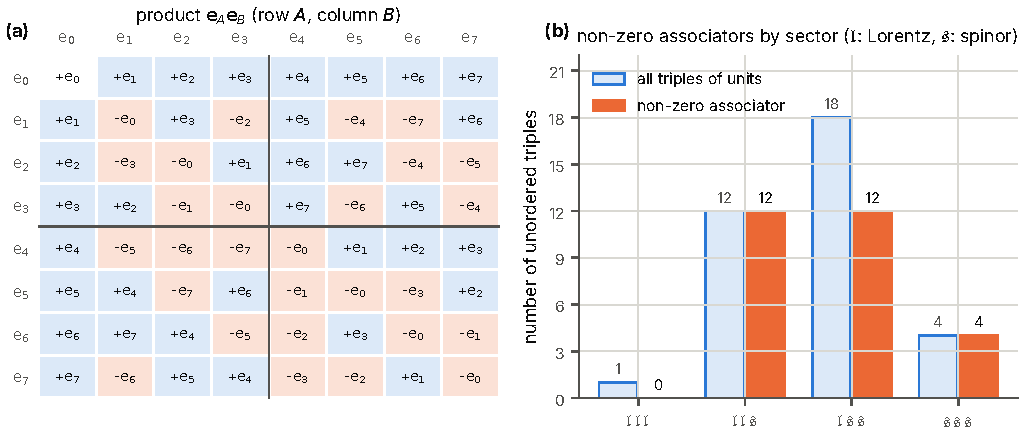
\includegraphics[width=\textwidth]{../figures/fig_sl_tables.pdf}
\caption{(a) The product $\mathbf e_p\mathbf e_{p'}$ of the units of $\mathbb B_{\rm LL}$ (row: left
factor; column: right factor; orange: a minus sign), from Eq.~(\ref{eq:cd}); the lines separate the
quaternion units $\mathbf e_0,\dots,\mathbf e_3$ from $\mathbf e_4,\dots,\mathbf e_7$. (b) The
unordered triples of distinct imaginary units, sorted by how many lie in the Lorentz part
$\mathfrak l_{\rm LL}$ (units $\mathbf e_1$, $\mathbf e_2$, $\mathbf e_3$) and how many in the spinor
charges $\mathfrak s_{\rm LL}$ (units $\mathbf e_4,\dots,\mathbf e_7$), and the number with a non-zero
associator: 168 ordered triples of units in all (check A-2).}
\label{fig:tables}
\end{figure*}

\subsection{Alternative, not associative}

The \emph{associator} $[\mathbf x,\mathbf y,\mathbf z]=(\mathbf x\mathbf y)\mathbf z-\mathbf x(\mathbf
y\mathbf z)$ measures the failure of associativity. For the bi-octonions:
\begin{enumerate}
\item The norm is multiplicative, $N_{\rm LL}(\mathbf x\mathbf y)=N_{\rm LL}(\mathbf x)N_{\rm LL}(\mathbf
y)$ (check A-3, exact on random bi-octonions with Gaussian-integer coefficients).
\item The associator is \emph{alternating}: it changes sign when two arguments are exchanged, and so
vanishes when two arguments are equal (A-1). An algebra with this property is called
\emph{alternative}; in it any two elements generate an associative subalgebra (Artin's
theorem~\cite{Schafer1966}).
\item The product is not associative: 168 of the 512 ordered triples of units have
a non-zero associator, the triples of three distinct imaginary units that do not lie in a common
quaternion subalgebra; for example $[\mathbf e_1,\mathbf e_2,\mathbf e_4]=2\mathbf e_7$ (A-2).
Figure~\ref{fig:tables}(b) sorts them.
\item The Moufang identities
$\mathbf z(\mathbf x(\mathbf z\mathbf y))=((\mathbf z\mathbf x)\mathbf z)\mathbf y$,
$((\mathbf y\mathbf z)\mathbf x)\mathbf z=\mathbf y(\mathbf z(\mathbf x\mathbf z))$ and
$(\mathbf z\mathbf x)(\mathbf y\mathbf z)=(\mathbf z(\mathbf x\mathbf y))\mathbf z$ hold (A-3).
\end{enumerate}
Because the associator is alternating, the six associators of Eq.~(\ref{eq:jacassoc}) are all equal
up to their signs, and the Jacobiator of the commutator is
\begin{equation}
\mathrm{Jac}_{\rm LL}(\mathbf x,\mathbf y,\mathbf z)=6\,[\mathbf x,\mathbf y,\mathbf z]
\label{eq:jac6}
\end{equation}
(A-4): the Jacobi identity fails exactly where associativity fails.

\subsection{The super-loop and its Malcev algebra}

A \emph{loop} is a set with a product, an identity element, and unique solutions of the equations
$\mathbf w\mathbf x=\mathbf y$ and $\mathbf x\mathbf w=\mathbf y$ for $\mathbf x$; a group is an
associative loop. A \emph{Moufang loop} obeys the Moufang identities~\cite{Moufang1935}. The unit
bi-octonions
\begin{equation}
\mathbb L_{\rm LL}=\{\mathbf w\in\mathbb B_{\rm LL}:\ N_{\rm LL}(\mathbf w)=1\}
\label{eq:loop}
\end{equation}
form a Moufang loop: the product of two of them is one of them (the norm is multiplicative), $\mathbf
e_0$ is the identity, $\bar{\mathbf w}$ is the inverse of $\mathbf w$, and $\mathbf w\mathbf x=\mathbf y$
has the unique solution $\mathbf x=\bar{\mathbf w}\mathbf y$, because $\bar{\mathbf w}(\mathbf w\mathbf
y)=(\bar{\mathbf w}\mathbf w)\mathbf y$ by alternativity. We call it the \emph{Lorentz super-loop}. It
is a complex manifold of complex dimension 7 (real dimension 14), and it contains $SL(2,\mathbb C)$,
the unit bi-quaternions, as a subgroup.

Just as a Lie group has a Lie algebra, a Moufang loop that is a smooth manifold has a tangent algebra
at the identity: the imaginary bi-octonions $\mathfrak m_{\rm LL}=\mathbb C\otimes{\rm Im}\,\mathbb O$
with the commutator (real dimension 14). It is not a Lie algebra, by Eq.~(\ref{eq:jac6}), but it is a
\emph{Malcev algebra}~\cite{Malcev1955,Sagle1961}: its bracket is bilinear and antisymmetric and obeys
the Malcev identity $\mathrm{Jac}_{\rm LL}(\mathbf x,\mathbf y,[\mathbf x,\mathbf z])=[\mathrm{Jac}_{\rm
LL}(\mathbf x,\mathbf y,\mathbf z),\mathbf x]$, which in a Lie algebra holds trivially. We verify it in
the linearized form, obtained by replacing $\mathbf x$ by $\mathbf x+\mathbf w$ and keeping the part
linear in $\mathbf w$,
\begin{align}
&\mathrm{Jac}_{\rm LL}(\mathbf x,\mathbf y,[\mathbf w,\mathbf z])+\mathrm{Jac}_{\rm LL}(\mathbf w,\mathbf y,[\mathbf x,\mathbf z])\nonumber\\
&\quad=[\mathrm{Jac}_{\rm LL}(\mathbf x,\mathbf y,\mathbf z),\mathbf w]+[\mathrm{Jac}_{\rm LL}(\mathbf w,\mathbf y,\mathbf z),\mathbf x],
\label{eq:malcev}
\end{align}
on all 2401 4-tuples of imaginary units (A-5). Malcev algebras are to analytic Moufang loops what Lie
algebras are to Lie groups~\cite{Malcev1955,Kuzmin1971,NagyStrambach2002}.

\subsection{No realization by operators}

\noindent\emph{Theorem R.} (a) Every linear map $\varrho_{\rm LL}$ from $\mathfrak m_{\rm LL}$ to the
linear operators on a vector space that turns brackets into commutators,
$\varrho_{\rm LL}([\mathbf x,\mathbf y])=\varrho_{\rm LL}(\mathbf x)\varrho_{\rm LL}(\mathbf
y)-\varrho_{\rm LL}(\mathbf y)\varrho_{\rm LL}(\mathbf x)$, is zero. (b) No one-to-one map of
$\mathbb L_{\rm LL}$ into the invertible operators on a vector space turns the product of the loop into
the product of operators.

\noindent\emph{Proof.} (a) Applying $\varrho_{\rm LL}$ to Eq.~(\ref{eq:jacobiator}) gives
$\varrho_{\rm LL}(\mathrm{Jac}_{\rm LL}(\mathbf x,\mathbf y,\mathbf z))=\mathrm{Jac}_{\rm
LL}(\varrho_{\rm LL}(\mathbf x),\varrho_{\rm LL}(\mathbf y),\varrho_{\rm LL}(\mathbf z))$, and the right
side vanishes by Eq.~(\ref{eq:jacassoc}), because the product of operators is associative (A-6). Hence
$\varrho_{\rm LL}$ vanishes on every Jacobiator. The Jacobiators of the real basis $\mathbf e_p$,
$i\mathbf e_p$ ($p=1,\dots,7$) of $\mathfrak m_{\rm LL}$ span a space of real dimension
14, all of $\mathfrak m_{\rm LL}$ (A-8); so $\varrho_{\rm LL}=0$. (b) Such a map would
send $(\mathbf e_1\mathbf e_2)\mathbf e_4=\mathbf e_7$ and $\mathbf e_1(\mathbf e_2\mathbf e_4)=-\mathbf
e_7$ to the same operator, because both products of operators are equal; it would not be one-to-one.
$\square$

In particular the left multiplications $L^{\rm LL}_{\mathbf x}:\mathbf y\mapsto\mathbf x\mathbf y$, real
$16\times16$ matrices, do not represent $\mathfrak m_{\rm LL}$: $[L^{\rm LL}_{\mathbf e_1},L^{\rm
LL}_{\mathbf e_4}]\neq L^{\rm LL}_{[\mathbf e_1,\mathbf e_4]}$ (A-7). Theorem R is the precise sense in
which the non-associativity is essential: no reformulation by operators, and so no Hilbert space of
states on which the super-loop acts linearly and faithfully, removes it. Hypotheses H-grp, H-op and
H-Lie fail for $\mathbb L_{\rm LL}$, and they fail together.

\section{The Lorentz super-loop}
\label{sec:superloop}

\subsection{Lorentz part and spinor charges}

The Malcev algebra splits into two parts, $\mathfrak m_{\rm LL}=\mathfrak l_{\rm LL}\oplus\mathfrak s_{\rm
LL}$. The \emph{Lorentz part} $\mathfrak l_{\rm LL}=\mathbb C\otimes{\rm Im}\,\mathbb H$ consists of the
imaginary bi-quaternions $\mathbf u$ (real dimension 6). With the rotation and boost generators
\begin{equation}
J^j_{\rm LL}=\tfrac12\mathbf e_j,\qquad K^j_{\rm LL}=\tfrac12 i\,\mathbf e_j\qquad(j=1,2,3)
\label{eq:jk}
\end{equation}
Eq.~(\ref{eq:quat}) gives the brackets of the Lorentz algebra $\mathfrak{so}(3,1)$ (check L-1):
\begin{align}
[J^j_{\rm LL},J^{j'}_{\rm LL}]&=\textstyle\sum_{j''}\epsilon^{\rm LL}_{jj'j''}J^{j''}_{\rm LL},\nonumber\\
[J^j_{\rm LL},K^{j'}_{\rm LL}]&=\textstyle\sum_{j''}\epsilon^{\rm LL}_{jj'j''}K^{j''}_{\rm LL},\label{eq:so31}\\
[K^j_{\rm LL},K^{j'}_{\rm LL}]&=-\textstyle\sum_{j''}\epsilon^{\rm LL}_{jj'j''}J^{j''}_{\rm LL}.\nonumber
\end{align}
Its Killing form $\mathrm{Kil}_{\rm LL}(\mathbf x,\mathbf y)=\mathrm{tr}(\mathrm{ad}\,\mathbf
x\,\mathrm{ad}\,\mathbf y)$ has three negative (rotations) and three positive (boosts) eigenvalues
(L-2; $\mathrm{Kil}_{\rm LL}(\mathbf e_1,\mathbf e_1)={}$-16,
$\mathrm{Kil}_{\rm LL}(i\mathbf e_1,i\mathbf e_1)={}$16), as for $\mathfrak{so}(3,1)$.
$\mathfrak l_{\rm LL}$ is a Lie subalgebra, the tangent algebra of the subgroup $SL(2,\mathbb C)$.

The \emph{spinor charges} are the elements $\mathbf b\,\mathbf e_4$ of $\mathfrak s_{\rm LL}=(\mathbb
C\otimes\mathbb H)\,\mathbf e_4$ (real dimension 8). By Eq.~(\ref{eq:cdspecial}), $\mathbf u(\mathbf
b\mathbf e_4)=(\mathbf b\mathbf u)\mathbf e_4$ and $(\mathbf b\mathbf e_4)\mathbf u=(\mathbf b\bar{\mathbf
u})\mathbf e_4=-(\mathbf b\mathbf u)\mathbf e_4$, so a Lorentz element acts on a spinor charge by
\begin{equation}
[\mathbf u,\mathbf b\,\mathbf e_4]=2(\mathbf b\mathbf u)\,\mathbf e_4=-2\,(W_{\rm LL}(\mathbf u)\mathbf b)\,\mathbf e_4,
\label{eq:twist}
\end{equation}
where $W_{\rm LL}(\mathbf u)\mathbf b=-\mathbf b\mathbf u$. The map $W_{\rm LL}$ is a representation of $\mathfrak l_{\rm LL}$,
$[W_{\rm LL}(\mathbf u_1),W_{\rm LL}(\mathbf u_2)]=W_{\rm LL}([\mathbf u_1,\mathbf u_2])$, because
$W_{\rm LL}(\mathbf u_1)W_{\rm LL}(\mathbf u_2)\mathbf b=\mathbf b\mathbf u_2\mathbf u_1$. It is the
\emph{Weyl spinor}: under $M_{\rm LL}$ the right multiplication by $\mathbf u$ acts on the rows of the
$2\times2$ matrix $M_{\rm LL}(\mathbf b)$, and $W_{\rm LL}(J^j_{\rm LL})$, $W_{\rm LL}(K^j_{\rm LL})$ act
on each row as the generators of the $(\tfrac12,0)$ representation (Sec.~\ref{sec:superfluid}). The two
rows are an \emph{isospin doublet}: left multiplication by a unit quaternion $\mathbf v$,
$\mathbf b\mapsto\mathbf v\mathbf b$, mixes them and commutes with $W_{\rm LL}$. The inner action
$\rho_{\rm LL}=-2W_{\rm LL}$ of Eq.~(\ref{eq:twist}) is \emph{not} a representation:
$[\rho_{\rm LL}(\mathbf u_1),\rho_{\rm LL}(\mathbf u_2)]=4W_{\rm LL}([\mathbf u_1,\mathbf u_2])=-2\rho_{\rm
LL}([\mathbf u_1,\mathbf u_2])$ (L-3).

Two spinor charges have, by Eq.~(\ref{eq:cdspecial}), the bracket
\begin{equation}
[\mathbf b\,\mathbf e_4,\mathbf b'\mathbf e_4]=\bar{\mathbf b}\mathbf b'-\bar{\mathbf b}'\mathbf b\ \in\ \mathfrak l_{\rm LL},
\label{eq:ss}
\end{equation}
an imaginary bi-quaternion, i.e.\ a Lorentz generator; these brackets span all of $\mathfrak l_{\rm
LL}$ (L-4). Spinor charges close into Lorentz generators. Figure~\ref{fig:superloop} summarizes the
structure.

\begin{figure}[t]
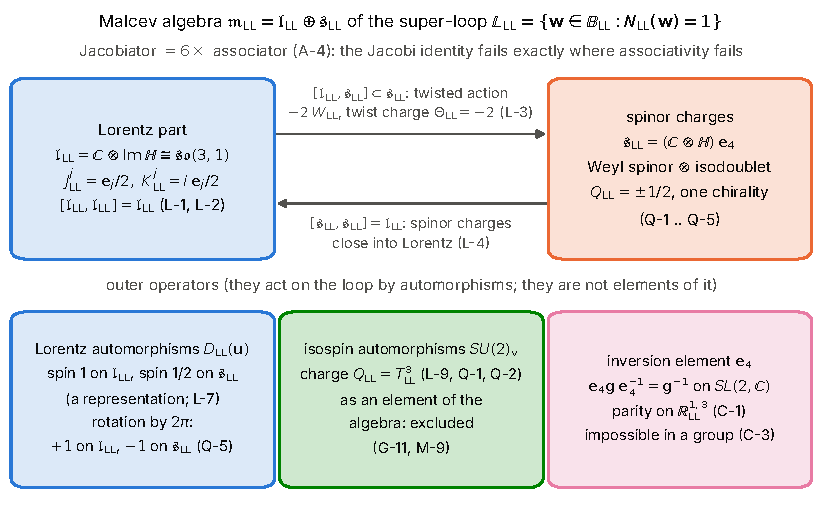
\includegraphics[width=\columnwidth]{../figures/fig_sl_superloop.pdf}
\caption{The Malcev algebra of the Lorentz super-loop: its Lorentz part $\mathfrak l_{\rm LL}$ and its
spinor charges $\mathfrak s_{\rm LL}$, their brackets, Eqs.~(\ref{eq:twist}) and~(\ref{eq:ss}), and the
outer operators of Sec.~\ref{sec:operators}, which act on the loop by automorphisms. The labels are
those of the machine checks.}
\label{fig:superloop}
\end{figure}

\subsection{The twist charge and the Jacobiators}

Define the \emph{twist charge} $\Theta_{\rm LL}$ as the linear map of $\mathfrak m_{\rm LL}$ that is $1$
on $\mathfrak l_{\rm LL}$ and $-2$ on $\mathfrak s_{\rm LL}$. With the Lorentz derivation $D_{\rm
LL}(\mathbf u)$ of Sec.~\ref{sec:operators}, which acts on $\mathfrak l_{\rm LL}$ by the commutator and on
$\mathfrak s_{\rm LL}$ by $W_{\rm LL}$, the inner action factors as $[\mathbf u,\cdot\,]=D_{\rm
LL}(\mathbf u)\circ\Theta_{\rm LL}$ (L-7). Suppose more generally that $\mathbf u$ acts on the spinor
charges by $\Theta_{\rm LL}W_{\rm LL}(\mathbf u)$ with any number $\Theta_{\rm LL}$. Then
\begin{align}
&\mathrm{Jac}_{\rm LL}(\mathbf u_1,\mathbf u_2,\mathbf b\,\mathbf e_4)\nonumber\\
&=\Big(\big(\Theta_{\rm LL}W_{\rm LL}([\mathbf u_1,\mathbf u_2])\nonumber\\
&\qquad-\Theta_{\rm LL}^2[W_{\rm LL}(\mathbf u_1),W_{\rm LL}(\mathbf u_2)]\big)\mathbf b\Big)\,\mathbf e_4\nonumber\\
&=(\Theta_{\rm LL}-\Theta_{\rm LL}^2)\,(W_{\rm LL}([\mathbf u_1,\mathbf u_2])\mathbf b)\,\mathbf e_4 ,
\label{eq:jacluu}
\end{align}
which vanishes for the Lie actions $\Theta_{\rm LL}=0$ (trivial) and $\Theta_{\rm LL}=1$ (the Weyl
representation) and equals $-6(W_{\rm LL}([\mathbf u_1,\mathbf u_2])\mathbf b)\mathbf e_4$ for the
super-loop, $\Theta_{\rm LL}=-2$ (L-5, exact on all 288 basis triples). The Jacobiators of three spinor
charges and of one Lorentz element with two spinor charges are non-zero as well, for example
$\mathrm{Jac}_{\rm LL}(\mathbf e_4,\mathbf e_5,\mathbf e_6)=-12\,\mathbf e_7$ (L-5).

\subsection{Theorem L: no Lie algebra does this}

\noindent\emph{Theorem L.} Let $\mathfrak l_{\rm LL}\oplus\mathfrak s_{\rm LL}$ carry a bracket that is
the Lorentz bracket on $\mathfrak l_{\rm LL}$, acts on $\mathfrak s_{\rm LL}$ covariantly, $[\mathbf
u,\mathbf b\mathbf e_4]=c^{\rm tw}_{\rm LL}(W_{\rm LL}(\mathbf u)\mathbf b)\mathbf e_4$, and has
$[\mathbf b\mathbf e_4,\mathbf b'\mathbf e_4]=c^{\rm sl}_{\rm LL}(\bar{\mathbf b}\mathbf b'-\bar{\mathbf
b}'\mathbf b)$, with complex numbers $c^{\rm tw}_{\rm LL}$, $c^{\rm sl}_{\rm LL}$. (Section~\ref{sec:classification}
shows that these are the most general Lorentz- and isospin-covariant brackets.) If the Jacobi identity
holds, then $c^{\rm sl}_{\rm LL}=0$: in a Lie algebra, bosonic spinor charges cannot close into the
Lorentz generators.

\noindent\emph{Proof.} By Eq.~(\ref{eq:jacluu}) with $\Theta_{\rm LL}=c^{\rm tw}_{\rm LL}$, the
Jacobi identity on $(\mathbf u_1,\mathbf u_2,\mathbf b\mathbf e_4)$ requires $c^{\rm tw}_{\rm LL}=0$ or
$1$. If $c^{\rm tw}_{\rm LL}=0$, the Jacobi identity on $(\mathbf u,\mathbf b\mathbf e_4,\mathbf b'\mathbf
e_4)$ reduces to $c^{\rm sl}_{\rm LL}[\bar{\mathbf b}\mathbf b'-\bar{\mathbf b}'\mathbf b,\mathbf u]=0$ for
every $\mathbf u$; the brackets span $\mathfrak l_{\rm LL}$ (L-4), whose center is zero, so $c^{\rm
sl}_{\rm LL}=0$. If $c^{\rm tw}_{\rm LL}=1$, the Jacobi identity on three spinor charges reads
$c^{\rm sl}_{\rm LL}\sum_{\rm cyc}(W_{\rm LL}(\bar{\mathbf b}\mathbf b'-\bar{\mathbf b}'\mathbf b)\mathbf
b'')\mathbf e_4=0$, the sum running over the three cyclic orders of $(\mathbf b,\mathbf b',\mathbf b'')$.
For $\mathbf b=\mathbf e_0$, $\mathbf b'=\mathbf e_1$, $\mathbf b''=\mathbf e_2$ the three brackets are
$2\mathbf e_1$, $-2\mathbf e_3$, $-2\mathbf e_2$, and the sum is $6c^{\rm sl}_{\rm LL}\mathbf e_7$; so $c^{\rm
sl}_{\rm LL}=0$. $\square$

Check L-6 verifies the last step on all basis triples, and the Gr\"obner-basis classification of
Sec.~\ref{sec:classification} confirms the theorem for all coefficients and extends it to the
Poincar\'e algebra and to an added isospin algebra (G-1, G-5, G-10). The same computation with
$c^{\rm tw}_{\rm LL}=-2$, $c^{\rm sl}_{\rm LL}=1$ gives $\mathrm{Jac}_{\rm LL}(\mathbf e_4,\mathbf
e_5,\mathbf e_6)=6c^{\rm tw}_{\rm LL}c^{\rm sl}_{\rm LL}\,\mathbf e_7=-12\,\mathbf e_7$, the value of
L-5: the super-loop violates the Jacobi identity, but it obeys the Malcev identity.

\section{Operators on the super-loop and their eigenvalues}
\label{sec:operators}

\subsection{Derivations and automorphisms}

An \emph{automorphism} of $\mathbb B_{\rm LL}$ is an invertible linear map that preserves the product;
a \emph{derivation} is its infinitesimal form, a linear map $\mathcal D_{\rm LL}$ with
$\mathcal D_{\rm LL}(\mathbf x\mathbf y)=(\mathcal D_{\rm LL}\mathbf x)\mathbf y+\mathbf x(\mathcal
D_{\rm LL}\mathbf y)$. Automorphisms map $\mathbb L_{\rm LL}$ to itself, so they are
symmetries of the super-loop that act on it from outside; they are linear operators on
$\mathbb B_{\rm LL}$ and, unlike the elements of the loop, compose associatively. Two families
matter (L-7):
\begin{align}
D_{\rm LL}(\mathbf u)(\mathbf a+\mathbf b\,\mathbf e_4)&=[\mathbf u,\mathbf a]+(-\mathbf b\mathbf u)\,\mathbf e_4,\label{eq:dlor}\\
D^{\rm v}_{\rm LL}(\mathbf t)(\mathbf a+\mathbf b\,\mathbf e_4)&=(\mathbf t\mathbf b)\,\mathbf e_4,\label{eq:diso}
\end{align}
for a Lorentz element $\mathbf u\in\mathfrak l_{\rm LL}$ and an isospin element $\mathbf t\in{\rm
Im}\,\mathbb H$. Both are derivations (checked on random pairs), they commute with each other, and
the isospin derivations vanish on $\mathbb C\otimes\mathbb H$. Integrated, they give the automorphisms
\begin{equation}
\varphi^{\rm LL}_{\mathbf g,\mathbf v}(\mathbf a+\mathbf b\,\mathbf e_4)=\mathbf g\mathbf a\bar{\mathbf g}+(\mathbf v\mathbf b\bar{\mathbf g})\,\mathbf e_4
\label{eq:aut}
\end{equation}
for unit bi-quaternions $\mathbf g$ (a Lorentz transformation) and $\mathbf v$ (an isospin rotation)
(L-9); together they form $(SL(2,\mathbb C)\times SL(2,\mathbb C))/\mathbb Z_2=SO(4,\mathbb C)$.
All derivations of $\mathbb B_{\rm LL}$ form the complex exceptional Lie algebra $\mathfrak g_2(\mathbb
C)$, of real dimension 28: the linear conditions for a derivation have rank 228 for the 256
entries of a real $16\times16$ matrix, and the inner derivations $[L^{\rm LL}_{\mathbf x},L^{\rm
LL}_{\mathbf y}]+[L^{\rm LL}_{\mathbf x},R^{\rm LL}_{\mathbf y}]+[R^{\rm LL}_{\mathbf x},R^{\rm
LL}_{\mathbf y}]$ (with the right multiplications $R^{\rm LL}_{\mathbf y}$) span 28
dimensions (L-8). The automorphism group is $\mathrm G_2(\mathbb C)$, and $SO(4,\mathbb C)$ is the part
of it that keeps $\mathbb C\otimes\mathbb H$ in place.

\subsection{The operators and their eigenvalues}

The super-loop carries the following operators, all built from Eqs.~(\ref{eq:dlor})
and~(\ref{eq:diso}); their eigenvalues are collected in Fig.~\ref{fig:charges}.

\emph{Isospin and electric charge.} The isospin generators $T^\iota_{\rm LL}=i\,D^{\rm v}_{\rm
LL}(\mathbf e_\iota/2)$ ($\iota=1,2,3$) are Hermitian and obey $[T^1_{\rm LL},T^2_{\rm LL}]=iT^3_{\rm
LL}$ and its cyclic permutations. We call the third one the \emph{electric charge},
$Q_{\rm LL}=T^3_{\rm LL}$. It has the eigenvalue 0 on $\mathbb C\otimes\mathbb H$ (four times) and the
eigenvalues $+\tfrac12$ and $-\tfrac12$ (twice each) on the spinor charges (Q-1); the isospin Casimir
$(T_{\rm LL})^2=\sum_\iota(T^\iota_{\rm LL})^2$ is 0 on $\mathbb C\otimes\mathbb H$ and
$\tfrac34=\tfrac12(\tfrac12+1)$ on the spinor charges, which are therefore an isospin doublet (Q-2).

\emph{Spin.} The Casimir of the rotations, $\mathrm{Cas}_{\rm LL}=-\sum_jD_{\rm LL}(J^j_{\rm LL})^2$, has
the eigenvalue 0 on $\mathbf e_0$ (spin 0), 2 on the Lorentz part (spin 1) and $\tfrac34$ on the
spinor charges (spin $\tfrac12$) (Q-3, exact).

\emph{Chirality.} Because $D_{\rm LL}$ is complex-linear in its argument and $K^j_{\rm LL}=iJ^j_{\rm
LL}$, every boost acts as $i$ times the corresponding rotation on every bi-octonion,
$D_{\rm LL}(K^j_{\rm LL})=i\,D_{\rm LL}(J^j_{\rm LL})$ (Q-4). A Lorentz multiplet on which the rotations
act with spin $\tfrac12$ (or 1) and the boosts as $i$ times the rotations is said to be of type
$(\tfrac12,0)$ (or $(1,0)$); with $-i$ in place of $i$ it is of type $(0,\tfrac12)$ (or $(0,1)$). So the
spinor charges are of type $(\tfrac12,0)$ and the Lorentz part of type $(1,0)$: the super-loop has one
chirality. The complex-conjugate super-loop, in which every coefficient is replaced by its complex
conjugate, has the other.

\emph{Spinor number.} The rotation by the angle $2\pi$ about the third axis, $\exp(2\pi D_{\rm
LL}(J^3_{\rm LL}))$, is $+1$ on $\mathbb C\otimes\mathbb H$ and $-1$ on the spinor charges, because
$iD_{\rm LL}(J^3_{\rm LL})$ has the integer eigenvalues $-1,0,0,1$ on the first and the eigenvalues
$\pm\tfrac12$ on the second (Q-5): the spinor charges are fermionic in their Lorentz quantum numbers,
although they are elements of an algebra with a commutator.

\emph{Twist charge.} $\Theta_{\rm LL}$, Sec.~\ref{sec:superloop}, is 1 on $\mathfrak l_{\rm LL}$ and
$-2$ on $\mathfrak s_{\rm LL}$. It is a new quantity: it measures by how much the inner action of the
Lorentz part fails to be a representation, Eq.~(\ref{eq:jacluu}), and Theorem M will show that $0$, $1$
and $-2$ are the only values that a Malcev algebra allows. Its value $-2$ appears directly in the loop:
conjugation by an element $\mathbf g$ of $SL(2,\mathbb C)$ acts on a spinor charge as
\begin{equation}
\mathbf g(\mathbf b\,\mathbf e_4)\bar{\mathbf g}=(\mathbf b\,\mathbf g^2)\,\mathbf e_4
\label{eq:conj}
\end{equation}
(Q-6; both orders of the two products agree), whereas the automorphism~(\ref{eq:aut}) acts as
$\mathbf b\mapsto\mathbf b\bar{\mathbf g}=\mathbf b\,\mathbf g^{-1}$: the loop's own conjugation turns a
spinor charge twice as fast and in the opposite sense.

\begin{figure}[t]
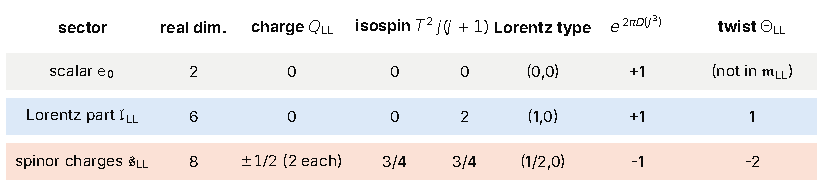
\includegraphics[width=\columnwidth]{../figures/fig_sl_charges.pdf}
\caption{Quantum numbers of the three sectors of $\mathbb B_{\rm LL}$ under the operators of
Sec.~\ref{sec:operators}: the electric charge $Q_{\rm LL}$, the isospin Casimir, the spin Casimir
$\mathrm{Cas}_{\rm LL}$, the Lorentz type, the spinor number $\exp(2\pi D_{\rm LL}(J^3_{\rm LL}))$ and the
twist charge $\Theta_{\rm LL}$ (checks Q-1 to Q-6, L-7).}
\label{fig:charges}
\end{figure}

\subsection{The inversion element}

The unit $\mathbf e_4$ itself is an element of the super-loop with $\mathbf e_4^2=-\mathbf e_0$ and
$\mathbf e_4^{-1}=-\mathbf e_4$. Conjugation by it acts on the bi-quaternions by
\begin{equation}
\mathbf e_4\,\mathbf a\,\mathbf e_4^{-1}=\bar{\mathbf a}
\label{eq:inversion}
\end{equation}
(C-1). On $SL(2,\mathbb C)$ this is the inversion $\mathbf g\mapsto\bar{\mathbf g}=\mathbf g^{-1}$, and on
the Minkowski space $\mathbb R^{1,3}_{\rm LL}$ of the Hermitian bi-quaternions $x^0_{\rm LL}\mathbf
e_0+i\sum_jx^j_{\rm LL}\mathbf e_j$ (Sec.~\ref{sec:manifolds}) it is the parity
$x^j_{\rm LL}\mapsto-x^j_{\rm LL}$. The union of $SL(2,\mathbb C)$ and $SL(2,\mathbb C)\,\mathbf e_4$ is
closed under the product, by Eq.~(\ref{eq:cd}):
\begin{align}
(\mathbf g\,\mathbf e_4)(\mathbf h\,\mathbf e_4)&=-\bar{\mathbf h}\mathbf g,\qquad \mathbf g(\mathbf h\,\mathbf e_4)=(\mathbf h\mathbf g)\,\mathbf e_4,\nonumber\\
(\mathbf g\,\mathbf e_4)\mathbf h&=(\mathbf g\bar{\mathbf h})\,\mathbf e_4
\label{eq:chein}
\end{align}
(C-2). It is a Moufang loop of the type constructed by Chein~\cite{Chein1974}, a ``double'' of the
Lorentz group, and it is not associative because $SL(2,\mathbb C)$ is not commutative.

Such an element cannot exist in a group. In a group, conjugation by an element is an automorphism, and
the inversion $\mathbf g\mapsto\mathbf g^{-1}$ of $SL(2,\mathbb C)$ is not one: for $\mathbf g=\mathbf e_1$
and $\mathbf h=\mathbf e_2$, $(\mathbf g\mathbf h)^{-1}=-\mathbf e_3$ but $\mathbf g^{-1}\mathbf
h^{-1}=+\mathbf e_3$ (C-3). In the loop, conjugation by $\mathbf e_4$ is not an automorphism of
$\mathbb B_{\rm LL}$ (C-4), and the inversion is realized by an element. This is a third way in which
the super-loop goes beyond what H-grp allows.

\section{Uniqueness: the classification of covariant brackets}
\label{sec:classification}

\subsection{The three families}

Is the super-loop an accident of the octonions, or the only way to let spinor charges close into
Lorentz generators? We answer the question for every bracket that is covariant under the Lorentz group
$SL(2,\mathbb C)$ and the isospin group $SU(2)_{\rm v}$, with the spinor charges a Weyl spinor that is an
isodoublet, in three families:
\begin{itemize}
\item $\mathcal F^{\rm A}_{\rm LL}$ on $\mathfrak l_{\rm LL}\oplus\mathfrak s_{\rm LL}$ (real dimension 14);
\item $\mathcal F^{\rm B}_{\rm LL}$ on $\mathfrak l_{\rm LL}\oplus\mathfrak p_{\rm LL}\oplus\mathfrak s_{\rm LL}$
(18), with the translations $\mathfrak p_{\rm LL}$, the Hermitian bi-quaternions $\mathbf r=\mathbf
r^\dagger$, on which $\mathfrak l_{\rm LL}$ acts by $[\mathbf u,\mathbf r]=\mathbf u\mathbf r+\mathbf
r\mathbf u^\dagger$ (the Lorentz action on four-vectors);
\item $\mathcal F^{\rm C}_{\rm LL}$ on $\mathfrak l_{\rm LL}\oplus\mathfrak{su}(2)\oplus\mathfrak s_{\rm
LL}$ (17), with isospin generators $\mathbf t\in{\rm Im}\,\mathbb H$ as elements.
\end{itemize}
The bracket of $\mathfrak l_{\rm LL}$ with itself is the Lorentz bracket, and the other brackets are
\begin{align}
[\mathbf u,\mathbf b\mathbf e_4]&=c^{\rm tw}_{\rm LL}(W_{\rm LL}(\mathbf u)\mathbf b)\,\mathbf e_4,\nonumber\\
[\mathbf r,\mathbf r']&=c^{\rm PP}_{\rm LL}(\mathbf r\bar{\mathbf r}'-\mathbf r'\bar{\mathbf r}),\nonumber\\
[\mathbf r,\mathbf b\mathbf e_4]&=c^{\rm Ps}_{\rm LL}(\mathbf b^*\bar{\mathbf r})\,\mathbf e_4,\nonumber\\
[\mathbf t,\mathbf t']&=c^{\rm TT}_{\rm LL}(\mathbf t\mathbf t'-\mathbf t'\mathbf t),\label{eq:families}\\
[\mathbf t,\mathbf b\mathbf e_4]&=c^{\rm Ts}_{\rm LL}(\mathbf t\mathbf b)\,\mathbf e_4,\nonumber\\
[\mathbf b\mathbf e_4,\mathbf b'\mathbf e_4]&=c^{\rm sl}_{\rm LL}(\bar{\mathbf b}\mathbf b'-\bar{\mathbf b}'\mathbf b)\nonumber\\
&\quad+c^{\rm sP}_{\rm LL}\,i(\bar{\mathbf b}\mathbf b'^*-\bar{\mathbf b}'\mathbf b^*)\nonumber\\
&\quad+\mathrm{Re}\big[c^{\rm sT}_{\rm LL}(\mathbf b\bar{\mathbf b}'-\mathbf b'\bar{\mathbf b})\big],\nonumber
\end{align}
where a term is present only if its target sector is ($\mathfrak p_{\rm LL}$ in $\mathcal F^{\rm B}_{\rm
LL}$, $\mathfrak{su}(2)$ in $\mathcal F^{\rm C}_{\rm LL}$), the real part in the last term is taken
coefficient by coefficient so that the result lies in ${\rm Im}\,\mathbb H$, $c^{\rm sP}_{\rm LL}$ and
$c^{\rm TT}_{\rm LL}$ are real, and the other coefficients are complex. The bi-octonions are
$\mathcal F^{\rm A}_{\rm LL}$ with $c^{\rm tw}_{\rm LL}=-2$, $c^{\rm sl}_{\rm LL}=1$
(Eqs.~(\ref{eq:twist}) and~(\ref{eq:ss}); check M-1).

\emph{These brackets are the most general covariant ones.} Complexify: the Lorentz algebra becomes two
commuting copies of $\mathfrak{sl}(2)$, and a complex representation is labelled by its two spins. The
spinor charges are $(\tfrac12,0)$ times an isodoublet, their complex conjugates $(0,\tfrac12)$, the
Lorentz part $(1,0)$ with its conjugate $(0,1)$, the translations $(\tfrac12,\tfrac12)$ and the
isospin generators $(0,0)$ times an isotriplet. A covariant real bilinear bracket is a sum of covariant
complex-bilinear maps between these representations and their conjugates, and the number of such
maps is the number of times the target occurs in the tensor product of the sources: the target
$(\tfrac12,0)$ occurs once in $(1,0)\otimes(\tfrac12,0)$ and never in $(0,1)\otimes(\tfrac12,0)$ [the
twist $c^{\rm tw}_{\rm LL}$]; $(1,0)$ times the
isosinglet occurs once in the antisymmetric square of $(\tfrac12,0)$ times the isodoublet, and never in
$(\tfrac12,0)\otimes(0,\tfrac12)$ [$c^{\rm sl}_{\rm LL}$]; the antisymmetric square of
$(\tfrac12,\tfrac12)$ is $(1,0)\oplus(0,1)$ [$c^{\rm PP}_{\rm LL}$]; $(\tfrac12,0)$ occurs once in
$(\tfrac12,\tfrac12)\otimes(0,\tfrac12)$ and never in $(\tfrac12,\tfrac12)\otimes(\tfrac12,0)$, so the
bracket of a translation with a spinor charge is antilinear in the spinor [$c^{\rm Ps}_{\rm LL}$];
$(\tfrac12,\tfrac12)$ times the isosinglet occurs once in $(\tfrac12,0)\otimes(0,\tfrac12)$ times
isodoublet $\otimes$ isodoublet, and only one real combination is antisymmetric [$c^{\rm sP}_{\rm LL}$];
the isotriplet occurs once in the antisymmetric square of the spinor charges (spin 0, antisymmetric,
times isospin 1, symmetric) [$c^{\rm sT}_{\rm LL}$]; and the isodoublet occurs once in isotriplet
$\otimes$ isodoublet [$c^{\rm Ts}_{\rm LL}$]. All other brackets between different sectors vanish by
covariance. Each complex coefficient counts two real ones, as the reality of the bracket requires.

\subsection{Method}

The Jacobi identity and the linearized Malcev identity~(\ref{eq:malcev}) are multilinear, so they hold
for all elements if they hold for all basis elements. Evaluated on integer elements, each component of
an identity is a polynomial in the real and imaginary parts of the coefficients (degree 2 for Jacobi,
3 for Malcev). The script \texttt{malcev\_groebner.py} evaluates the identities of each family on
random integer tuples until the linear span of the resulting polynomials stops growing, and computes
the reduced Gr\"obner basis~\cite{CoxLittleOShea2015} of the ideal they generate,
$\mathcal I^{\rm Jac}_{\rm LL}$ for Jacobi and $\mathcal I^{\rm Mal}_{\rm LL}$ for Malcev
(Table~\ref{tab:groebner}). Every polynomial found is a true consequence of the identity, so a
polynomial that lies in the ideal vanishes on every solution: the statements below are necessary
conditions, proved by ideal membership. To restrict to solutions on which a polynomial does not
vanish (for example $c^{\rm sl}_{\rm LL}\neq0$), the ideal is enlarged by that polynomial times an
auxiliary variable $w^{\rm sat}_{\rm LL}$, minus 1 (saturation). Conversely, the Rust command
\texttt{malcev} checks every solution found here on \emph{all} basis triples and 4-tuples, in exact
integer arithmetic, so the solutions are proved to satisfy the identities (checks M-1 to M-9).

\begin{table}[t]
\caption{The constraint ideals: number of independent polynomials, of random integer tuples used, and
of elements of the reduced Gr\"obner basis (grevlex order), for each family and identity.}
\label{tab:groebner}
\begin{ruledtabular}
\begin{tabular}{lcccc}
family & identity & polynomials & tuples & basis\\
\hline
$\mathcal F^{\mathrm{A}}_{\mathrm{LL}}$ & Jacobi & 6 & 13 & 5 \\
$\mathcal F^{\mathrm{A}}_{\mathrm{LL}}$ & Malcev & 8 & 13 & 9 \\
$\mathcal F^{\mathrm{B}}_{\mathrm{LL}}$ & Jacobi & 19 & 15 & 19 \\
$\mathcal F^{\mathrm{B}}_{\mathrm{LL}}$ & Malcev & 85 & 20 & 20 \\
$\mathcal F^{\mathrm{C}}_{\mathrm{LL}}$ & Jacobi & 12 & 15 & 25 \\
$\mathcal F^{\mathrm{C}}_{\mathrm{LL}}$ & Malcev & 43 & 16 & 113 \\
\end{tabular}
\end{ruledtabular}
\end{table}

\subsection{Theorem M}

\noindent\emph{Theorem M.} (a) In $\mathcal F^{\rm A}_{\rm LL}$, the Jacobi identity forces $c^{\rm
sl}_{\rm LL}=0$ and $c^{\rm tw}_{\rm LL}\in\{0,1\}$ (G-1, G-2; Theorem L). (b) The Malcev identity
forces $c^{\rm tw}_{\rm LL}(c^{\rm tw}_{\rm LL}-1)(c^{\rm tw}_{\rm LL}+2)=0$, a cubic whose only roots
are $0$, $1$ and $-2$ (G-3); all three give Malcev algebras, the first two Lie algebras (M-2): the
value $-2$ is Carlsson's non-Lie Malcev module of $\mathfrak{sl}(2)$~\cite{Carlsson1976,Elduque1990}. If
$c^{\rm sl}_{\rm LL}\neq0$, then $c^{\rm tw}_{\rm LL}=-2$ (G-4), and the rescaling $\mathbf
b\mapsto\lambda^{\rm sc}_{\rm LL}\mathbf b$ by a complex number, which maps $c^{\rm sl}_{\rm LL}$ to
$(\lambda^{\rm sc}_{\rm LL})^2c^{\rm sl}_{\rm LL}$, makes $c^{\rm sl}_{\rm LL}=1$: the algebra is
$\mathfrak m_{\rm LL}$, the commutator algebra of the bi-octonions (M-1). Every other member fails
(M-3). (c) In $\mathcal F^{\rm B}_{\rm LL}$, even the Malcev identity forces $c^{\rm sl}_{\rm LL}=0$:
with translations present, spinor charges never close into Lorentz generators (G-7). The only non-Lie
Malcev member is $c^{\rm tw}_{\rm LL}=-2$ with all other coefficients zero (G-8, G-9, M-4, M-7): spinor
charges that commute with each other and with the translations, with the twisted Lorentz action. The
Lie members are (i) the Poincar\'e algebra with commuting spinor charges, (ii) the Poincar\'e algebra
with $[\mathfrak s_{\rm LL},\mathfrak s_{\rm LL}]\subset\mathfrak p_{\rm LL}$ ($c^{\rm sP}_{\rm LL}\neq0$),
and (iii) for $c^{\rm PP}_{\rm LL}=\lvert c^{\rm Ps}_{\rm LL}\rvert^2>0$ the de Sitter algebra
$\mathfrak{so}(4,1)$ (signature of its Killing form: 4 positive, 6 negative; M-6) acting on its real
spinor representation, with $[\mathfrak p_{\rm LL},\mathfrak s_{\rm LL}]\neq0$ and $[\mathfrak s_{\rm
LL},\mathfrak s_{\rm LL}]=0$ (G-5, G-6, M-5). (d) In $\mathcal F^{\rm C}_{\rm LL}$, the Jacobi identity
forces $c^{\rm sl}_{\rm LL}=0$ (G-10); and if $c^{\rm sl}_{\rm LL}\neq0$, the Malcev identity forces
$c^{\rm Ts}_{\rm LL}=c^{\rm sT}_{\rm LL}=0$ and $c^{\rm tw}_{\rm LL}=-2$ (G-11, G-12, M-8, M-9): isospin
cannot act on the spinor charges as an element of the algebra; it acts on the super-loop only from
outside, as the automorphisms~(\ref{eq:aut}).

The reduced Gr\"obner bases of $\mathcal F^{\rm A}_{\rm LL}$ illustrate the proof (variables: the real
and imaginary parts \texttt{ctw\_re}, \texttt{ctw\_im}, \texttt{csl\_re}, \texttt{csl\_im} of $c^{\rm
tw}_{\rm LL}$ and $c^{\rm sl}_{\rm LL}$). For the Jacobi identity the basis contains \texttt{csl\_re}
and \texttt{csl\_im} themselves---so $c^{\rm sl}_{\rm LL}=0$ on every solution---together with the real
and imaginary parts of $c^{\rm tw}_{\rm LL}(c^{\rm tw}_{\rm LL}-1)$. Case (ii) of (c) is a bosonic
analogue of supersymmetry: spinor charges whose brackets are translations. It is a Lie algebra, so the
theorem of Coleman and Mandula applies to it if it is to be a symmetry of a scattering matrix, and
Haag, {\L}opusza\'nski and Sohnius showed that the anticommutator, not the commutator, is the
consistent choice there. Case (iii) lives in de Sitter space, where the hypotheses H-dyn on a scattering
matrix are not available. Neither is a counterexample in the sense of this paper; they are listed to
make the classification complete.

\begin{figure}[t]
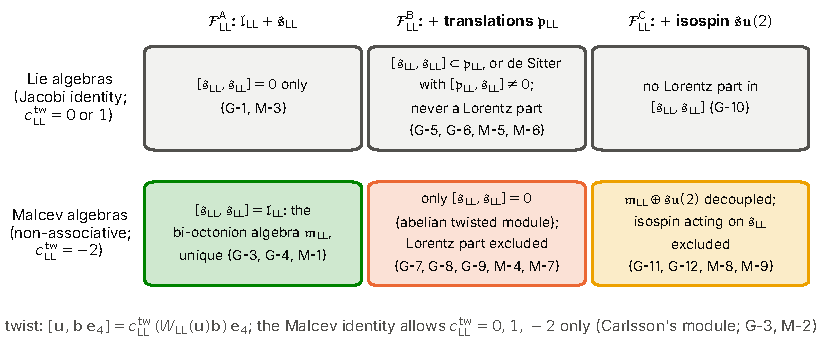
\includegraphics[width=\columnwidth]{../figures/fig_sl_classification.pdf}
\caption{Theorem M: what the bracket of two spinor charges can contain, for Lie algebras (top) and for
non-Lie Malcev algebras (bottom), in the three families. Green: the super-loop $\mathfrak m_{\rm LL}$,
unique; orange: the abelian twisted module of the Poincar\'e algebra; yellow: isospin decouples. The
labels are those of the checks.}
\label{fig:classification}
\end{figure}

\section{Manifolds that carry the super-loop}
\label{sec:manifolds}

The super-loop is itself a manifold, and it acts on others. Figure~\ref{fig:manifolds} collects the
manifolds that we identify; each statement is a machine check.

\emph{The $7{+}1$ Minkowski space.} The Hermitian bi-octonions, $\mathbf x^\dagger=\mathbf x$, are the
elements $\mathbf x=x^0_{\rm LL}\mathbf e_0+i\sum_{p=1}^7x^p_{\rm LL}\mathbf e_p$ with real coordinates
$x^p_{\rm LL}$. On them the norm is real,
\begin{equation}
N_{\rm LL}(\mathbf x)=(x^0_{\rm LL})^2-\textstyle\sum_{p=1}^7(x^p_{\rm LL})^2 ,
\label{eq:r17}
\end{equation}
with one positive and seven negative signs: they form the Minkowski space $\mathbb R^{1,7}_{\rm LL}$
of $7{+}1$ dimensions (N-1). The Hermitian bi-quaternions ($p\le3$) form the Minkowski space $\mathbb
R^{1,3}_{\rm LL}$ of $3+1$ dimensions, on which $SL(2,\mathbb C)$ acts by $\mathbf x\mapsto\mathbf
g\mathbf x\mathbf g^\dagger$: the familiar action of the Lorentz group on four-vectors. The
conjugations $\mathbf x\mapsto\mathbf g\mathbf x\mathbf g^\dagger$ of $\mathbb R^{1,7}_{\rm LL}$ by the
one-parameter families $\mathbf g=\exp(\theta_{\rm LL}\mathbf e_p)$ (rotations) and $\mathbf
g=\exp(\theta_{\rm LL}i\mathbf e_p)$ (boosts) of loop elements, $p=1,\dots,7$, have the generators
$\mathbf x\mapsto[\mathbf e_p,\mathbf x]$ and $\mathbf x\mapsto i(\mathbf e_p\mathbf x+\mathbf x\mathbf
e_p)$; they preserve Eq.~(\ref{eq:r17}), and the Lie algebra they generate is all of $\mathfrak{so}(1,7)$,
of dimension 28 (N-4). (The products are unambiguous: by Artin's theorem the subalgebra generated by
$\mathbf e_p$ and $\mathbf x$ is associative.)

\emph{Conjugation by the loop is not a group action.} Restricted to the loop's own Lorentz subgroup
($p=1,2,3$), the six generators preserve $\mathbb R^{1,3}_{\rm LL}$ and act on it as
$\mathfrak{so}(3,1)$, but on $\mathbb R^{1,7}_{\rm LL}$ they generate a Lie algebra of dimension
$9=6+3$ (N-5): on the four directions $i\mathbf e_4,\dots,i\mathbf e_7$ the boosts act trivially and the
rotations by the twisted action of Eq.~(\ref{eq:twist}), and the commutators separate an extra
$\mathfrak{so}(3)$ that acts on these directions alone. A group action would give back a Lie algebra of
dimension 6. This is the geometric face of the twist charge.

\emph{The $4{+}4$ manifold.} The real subspace $\mathbb O^{\rm s}_{\rm LL}=\mathbb H+(i\mathbb H)\mathbf
e_4$ of $\mathbb B_{\rm LL}$ is closed under the product, and the map from the split Cayley-Dickson
algebra (pairs of real quaternions with the sign $+1$ in place of the $-1$ of Eq.~(\ref{eq:cd})) that
sends the pair $(\mathbf a,\mathbf b)$ to $\mathbf a+(i\mathbf b)\mathbf e_4$ is an isomorphism onto it
(N-2): $\mathbb O^{\rm s}_{\rm LL}$ is the algebra of \emph{split octonions}, and the norm has on it the
signature $(4,4)$. Its unit elements form the pseudo-sphere $S^{3,4}_{\rm LL}$, a Moufang loop and the
$4{+}4$ real form of the super-loop. Inside its imaginary part, $\mathbf e_1$, $i\mathbf e_4$ and
$i\mathbf e_5$ span the Lie algebra $\mathfrak{sl}(2,\mathbb R)=\mathfrak{so}(2,1)$ (Killing form: two
positive, one negative; N-9): on the real $4{+}4$ manifold the Lorentz part of the super-loop is the
Lorentz group of $2+1$ dimensions, $SL(2,\mathbb R)=Spin(2,1)$, and $SO(3,1)$ needs the complex form.
The space of spinor charges is a second $4{+}4$ space: $\mathrm{Re}\,N_{\rm LL}$ and $\mathrm{Im}\,N_{\rm
LL}$ are, on $\mathfrak s_{\rm LL}$, two quadratic forms of signature $(4,4)$, both invariant under the
automorphisms~(\ref{eq:aut}) (N-3).

\emph{The super-loop manifold.} $\mathbb L_{\rm LL}$, Eq.~(\ref{eq:loop}), is a complex quadric of real
dimension 14; as a homogeneous space it is $Spin(7,\mathbb C)/\mathrm G_2(\mathbb C)$. It is
\emph{parallelizable}: the vector fields $X^{\rm LL}_{\mathbf x}(\mathbf w)=\mathbf w\mathbf x$ for the 14
real imaginary directions $\mathbf x$ are tangent to it, $N_{\rm LL}(\mathbf w,\mathbf w\mathbf x)=0$, and
form a frame at every point. Their Lie brackets are
\begin{equation}
[X^{\rm LL}_{\mathbf x},X^{\rm LL}_{\mathbf y}](\mathbf w)=\mathbf w[\mathbf x,\mathbf y]+2[\mathbf w,\mathbf x,\mathbf y]
\label{eq:frames}
\end{equation}
(N-7; it follows from $(\mathbf w\mathbf x)\mathbf y-(\mathbf w\mathbf y)\mathbf x$ and alternativity).
At the identity this is the Malcev bracket; elsewhere the associator makes the structure functions
depend on the point. On a Lie group the frame fields of the group's own multiplication have constant
structure functions: $\mathbb L_{\rm LL}$ is a parallelizable manifold that carries no Lie group
structure compatible with its product. Its compact real form, the unit octonions, is the seven-sphere
$S^7_{\rm LL}$; the products $L^{\rm LL}_{\mathbf e_p}L^{\rm LL}_{\mathbf e_{p'}}$ ($p<p'$) span
$\mathfrak{spin}(7)$, of dimension 21, whose stabilizer of $\mathbf e_0$ is $\mathfrak g_2$ (14), so that
$S^7_{\rm LL}=Spin(7)/\mathrm G_2$ (N-8)~\cite{Baez2002}.

\emph{The linear action closes into Lie groups.} The left multiplications by the imaginary
bi-octonions generate $\mathfrak{so}(8,\mathbb C)$ (real dimension 56), those by the imaginary octonions
$\mathfrak{so}(8)$, and those by the imaginary split octonions on $\mathbb O^{\rm s}_{\rm LL}$
$\mathfrak{so}(4,4)$ (N-6). Any \emph{linear} action of the loop on a vector space generates a Lie
group, in agreement with Theorem R; the non-associative structure lives in the product of the loop,
not in its linear action. Section~\ref{sec:renorm} uses this fact.

\begin{figure}[t]
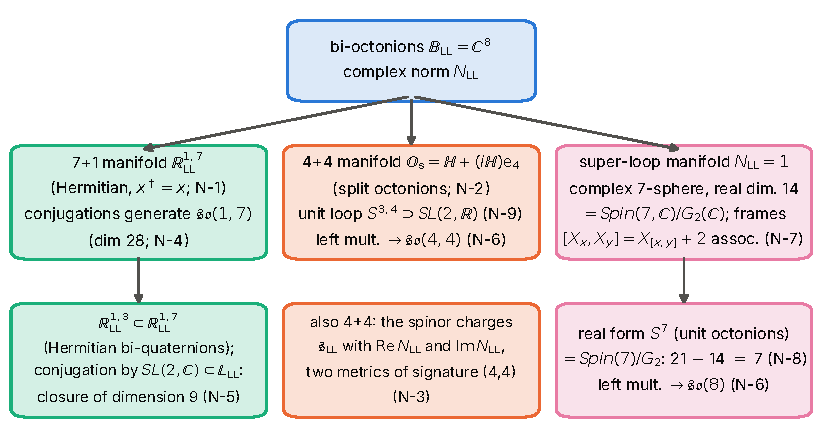
\includegraphics[width=\columnwidth]{../figures/fig_sl_manifolds.pdf}
\caption{The manifolds that carry the super-loop: $\mathbb R^{1,7}_{\rm LL}$ and $\mathbb R^{1,3}_{\rm
LL}$ (conjugation), the split octonions $\mathbb O^{\rm s}_{\rm LL}$ ($4{+}4$), the space of spinor charges
with its two $(4,4)$ forms, the super-loop manifold and its compact real form $S^7_{\rm LL}$. The
labels are those of the checks.}
\label{fig:manifolds}
\end{figure}

\section{The counterexamples}
\label{sec:counterexamples}

We collect the counterexamples to the conclusion of the no-go theorems, each with the hypothesis that
fails and the reason why it must fail.

\emph{Counterexample 1: the Lorentz super-loop.} $\mathbb L_{\rm LL}$ contains the Lorentz group
$SL(2,\mathbb C)$ and eight spinor charges that carry internal quantum numbers---isospin $\tfrac12$
and electric charge $\pm\tfrac12$---and Lorentz quantum numbers---spin $\tfrac12$, one chirality,
spinor number $-1$. The bracket of two spinor charges is a Lorentz generator, Eq.~(\ref{eq:ss}), so the
structure is not a direct product of a Lorentz part and an internal part. For a Lie algebra this is
impossible (Theorem L); for a non-associative structure it happens, and uniquely (Theorem M(b)).
Hypotheses that fail: H-grp (the loop is not associative), H-op and H-Lie (Theorem R: there is no
realization by operators, and the Jacobi identity fails, Eq.~(\ref{eq:jac6})).

\emph{Counterexample 2: inversion as an element.} The unit $\mathbf e_4$ of the super-loop acts on
$SL(2,\mathbb C)$ by the inversion and on $\mathbb R^{1,3}_{\rm LL}$ by the parity, Eq.~(\ref{eq:inversion}),
and together with $SL(2,\mathbb C)$ it generates a Moufang loop, Eq.~(\ref{eq:chein}). No group contains
such an element (check C-3). Hypothesis that fails: H-grp.

\emph{Counterexample 3: a parallelizable manifold of Lorentz and spinor directions without a group
structure.} The super-loop manifold carries frame fields along the six Lorentz and the eight spinor
directions whose brackets, Eq.~(\ref{eq:frames}), mix the two kinds and depend on the point through the
associator. Its real forms, $S^7_{\rm LL}$ and the pseudo-sphere $S^{3,4}_{\rm LL}$ of the $4{+}4$ manifold,
have the same property. Hypothesis that fails: H-grp (and H-Lie for the frames).

\emph{Counterexample 4, weaker: spinor charges of the Poincar\'e algebra with a twisted Lorentz action.}
With translations present, no Malcev algebra of our families lets spinor charges close into Lorentz
generators (Theorem M(c)); the only non-Lie extension is the abelian module on which the Lorentz
generators act with the twist $-2$: spinor charges that commute with the translations and with each
other but transform under a Lorentz action that is not a representation (check M-4). Its untwisted
version is a Lie algebra, which Coleman and Mandula exclude as a symmetry of a scattering matrix through
H-op and H-dyn; the twisted version escapes H-Lie as well, but, having no operator realization, it is
not a symmetry of a scattering matrix of an ordinary quantum theory either.

What none of these is: a symmetry of the scattering matrix of a relativistic quantum field theory on a
Hilbert space. Theorem R forbids it. The counterexamples show which conclusions of the no-go theorems
rest on associativity alone: the separation of Lorentz and internal generators (Theorem L versus
Counterexample 1) and the realization of every element by an automorphism (Counterexample 2).

\section{The spin-zero superfluid of the spinor charges}
\label{sec:superfluid}

\subsection{The field content from the bi-octonion product}

Write a spinor charge $\mathbf b\,\mathbf e_4$ through the $2\times2$ matrix $M_{\rm LL}(\mathbf b)$ of
Sec.~\ref{sec:bioct}. The Lorentz derivation~(\ref{eq:dlor}) multiplies $\mathbf b$ by $-\mathbf u$ from
the right, which acts within each row of $M_{\rm LL}(\mathbf b)$; the isospin derivation~(\ref{eq:diso})
multiplies from the left, which mixes the two rows. Define the $2\times2$ matrix
\begin{equation}
\psi'_{\rm LL}=\mathsf E_{\rm LL}^{-1}M_{\rm LL}(\mathbf b)^T,\qquad \mathsf E_{\rm LL}=i\sigma^{\rm LL}_2 .
\label{eq:psiprime}
\end{equation}
Its first column (isospin up) and its second column (isospin down) are Weyl spinors: on each column the
Lorentz derivations act as $D_{\rm LL}(J^j_{\rm LL})=-\tfrac{i}{2}\sigma^{\rm LL}_j$ and $D_{\rm
LL}(K^j_{\rm LL})=+\tfrac12\sigma^{\rm LL}_j$, and the isospin generators $T^\iota_{\rm LL}$ act on the
column index as $\tfrac12\tau^{\rm LL}_\iota$ (check S-0; the step uses $\mathsf E_{\rm
LL}^{-1}(\sigma^{\rm LL}_j)^T\mathsf E_{\rm LL}=-\sigma^{\rm LL}_j$).

In the chiral basis the Dirac matrices are $\gamma^0_{\rm LL}=\begin{pmatrix}0&\sigma^{\rm
LL}_0\\\sigma^{\rm LL}_0&0\end{pmatrix}$, $\gamma^j_{\rm LL}=\begin{pmatrix}0&\sigma^{\rm
LL}_j\\-\sigma^{\rm LL}_j&0\end{pmatrix}$, with the chirality matrix $\gamma^{\rm ch}_{\rm LL}=i\gamma^0_{\rm
LL}\gamma^1_{\rm LL}\gamma^2_{\rm LL}\gamma^3_{\rm LL}=\mathrm{diag}(-1,-1,1,1)$ and the charge-conjugation
matrix $C_{\rm LL}=i\gamma^2_{\rm LL}\gamma^0_{\rm LL}$~\cite{PeskinSchroeder1995}. The spinor charges, on
which $D_{\rm LL}(K^j_{\rm LL})=+\tfrac12\sigma^{\rm LL}_j$, are the lower block ($\gamma^{\rm ch}_{\rm
LL}=+1$); the complex-conjugate super-loop, on which the boosts act with the opposite sign, supplies the
upper block. The Dirac matrices intertwine these spinor generators with the action of the loop's
conjugations on $\mathbb R^{1,3}_{\rm LL}$: for each of the six generators, $[\gamma^p_{\rm LL},\cdot\,]$
reproduces the vector action $\mathcal V_{\rm LL}$ (all 24 relations of S-0). The field of the
spinor charges is therefore a \emph{Dirac isodoublet} $\Psi_{\rm LL}$ with 8 components (Dirac $\otimes$
isospin), with electric charges $Q_{\rm LL}=\pm\tfrac12$. Its components have spinor number $-1$, so, by
the spin-statistics theorem of relativistic quantum field theory, $\Psi_{\rm LL}$ is a fermion field: its
components anticommute.

The Hamiltonian is that of free Dirac particles of mass $m_{\rm LL}$ at the chemical potential $\mu_{\rm
LL}$, with an attractive contact interaction in the spin-zero channels of Theorem SF1 below,
\begin{equation}
\mathcal H^{\rm sf}_{\rm LL}=\sum_{\vec q_{\rm LL}}\Psi^\dagger_{\rm LL}(\mathsf h_{\rm LL}-\mu_{\rm LL})\Psi_{\rm LL}-\tfrac14G_{\rm LL}\sum_\iota(\Pi^\iota_{\rm LL})^\dagger\Pi^\iota_{\rm LL},
\label{eq:ham}
\end{equation}
with $\mathsf h_{\rm LL}(\vec q_{\rm LL})=\sum_j\alpha^j_{\rm LL}q^j_{\rm LL}+\beta_{\rm LL}m_{\rm LL}$
(times $\sigma^{\rm LL}_0$ on the isospin index), $\alpha^j_{\rm LL}=\gamma^0_{\rm LL}\gamma^j_{\rm LL}$,
$\beta_{\rm LL}=\gamma^0_{\rm LL}$, and the pair operators $\Pi^\iota_{\rm LL}=\sum_{\vec q_{\rm
LL}}\Psi_{\rm LL}(\vec q_{\rm LL})^T\mathsf K^\iota_{\rm LL}\Psi_{\rm LL}(-\vec q_{\rm LL})$, which annihilate
two spinor charges of opposite momenta. Momentum sums run over $q_{\rm LL}<\Lambda_{\rm LL}$.

\subsection{The spin-zero channels}

\noindent\emph{Theorem SF1.} The antisymmetric $8\times8$ matrices $\mathsf K$ for which the pair
$\Psi^T_{\rm LL}\mathsf K\Psi_{\rm LL}$ is Lorentz invariant form a complex space of dimension 6, spanned by
\begin{equation}
\mathsf K^\iota_{\rm LL}=C_{\rm LL}\gamma^{\rm ch}_{\rm LL}\otimes\mathsf E_{\rm LL}\tau^{\rm LL}_\iota,\quad \mathsf K'^\iota_{\rm LL}=C_{\rm LL}\otimes\mathsf E_{\rm LL}\tau^{\rm LL}_\iota
\label{eq:channels}
\end{equation}
($\iota=1,2,3$; scalar $0^+$ and pseudoscalar $0^-$). Every spin-zero s-wave pair of spinor charges is
an isospin \emph{triplet}, with the electric charges $+1$, $0$, $-1$.

\noindent\emph{Proof.} The Lorentz-invariant bilinear forms of a Dirac spinor are those of
$(\tfrac12,0)\otimes(\tfrac12,0)$ and $(0,\tfrac12)\otimes(0,\tfrac12)$, one each, spanned by $C_{\rm
LL}=\mathrm{diag}(\mathsf E_{\rm LL},-\mathsf E_{\rm LL})$ and $C_{\rm LL}\gamma^{\rm ch}_{\rm
LL}=-\mathrm{diag}(\mathsf E_{\rm LL},\mathsf E_{\rm LL})$; both are antisymmetric. For anticommuting
components only the antisymmetric part of $\mathsf K$ contributes, so the isospin factor must be
symmetric. The symmetric $2\times2$ matrices are spanned by the three matrices $\mathsf E_{\rm
LL}\tau^{\rm LL}_\iota$, which transform as an isospin vector; the remaining matrix $\mathsf E_{\rm LL}$,
the isosinglet, is antisymmetric and drops out. $\square$ (Check S-1 computes the dimension 6 directly and
the isospin Casimir 2 of every channel.) The pair $\mathsf K^3_{\rm LL}$ joins an isospin-up with an
isospin-down charge (charge 0), and $\mathsf K^1_{\rm LL}\mp i\mathsf K^2_{\rm LL}$ joins two up or two
down charges (charge $\pm1$) (S-2).

\subsection{Mean field and spectra}

The order parameter is the complex isospin vector $\vec d_{\rm LL}$ with $d^\iota_{\rm
LL}=-\tfrac12G_{\rm LL}\langle\Pi^\iota_{\rm LL}\rangle$. Replacing the product of pair operators in
Eq.~(\ref{eq:ham}) by its mean-field form gives, for each momentum, the Bogoliubov-de Gennes matrix
$\mathsf H_{\rm LL}$ on the Nambu spinor $(\Psi_{\rm LL}(\vec q_{\rm LL}),\Psi^*_{\rm LL}(-\vec q_{\rm LL}))$,
\begin{equation}
\mathsf H_{\rm LL}=\begin{pmatrix}\mathsf h_{\rm LL}(\vec q_{\rm LL})-\mu_{\rm LL}&\mathsf P_{\rm LL}\\\mathsf P_{\rm LL}^\dagger&-(\mathsf h_{\rm LL}(-\vec q_{\rm LL})-\mu_{\rm LL})^T\end{pmatrix},
\label{eq:bdg}
\end{equation}
with $\mathsf P_{\rm LL}=\sum_\iota d^\iota_{\rm LL}(\mathsf K^\iota_{\rm LL})^\dagger$, and the grand potential
per volume at zero temperature, measured from the normal state,
\begin{align}
\Omega_{\rm LL}={}&\frac{\lvert\vec d_{\rm LL}\rvert^2}{G_{\rm LL}}-\frac12\int\!\frac{d^3q_{\rm LL}}{(2\pi)^3}\sum_{\rm pos}\big(\text{eigenvalues of }\mathsf H_{\rm LL}\big)\nonumber\\
&-(\ldots)_{\vec d_{\rm LL}=0},
\label{eq:omega}
\end{align}
the sum running over the positive eigenvalues.

\noindent\emph{Theorem SF2.} In the scalar channel the positive eigenvalues of $\mathsf H_{\rm LL}$ are
$E^+_{\rm LL}$ and $E^-_{\rm LL}$ for each of the two gaps
\begin{equation}
(\Delta^\pm_{\rm LL})^2=\lvert\vec d_{\rm LL}\rvert^2(1\pm\zeta_{\rm LL}),\qquad \zeta_{\rm LL}=\frac{\lvert\vec d_{\rm LL}\times\vec d^{\,*}_{\rm LL}\rvert}{\lvert\vec d_{\rm LL}\rvert^2},
\label{eq:gaps}
\end{equation}
each twice, where $E^\pm_{\rm LL}=[(\varepsilon_{\rm LL}\pm\mu_{\rm LL})^2+\Delta_{\rm LL}^2]^{1/2}$ with
$\Delta_{\rm LL}$ replaced by the gap, and $\varepsilon_{\rm LL}=(q_{\rm LL}^2+m_{\rm LL}^2)^{1/2}$. A state
with $\zeta_{\rm LL}=0$ is called \emph{unitary}, as in the theory of superfluid
$^3$He~\cite{BalianWerthamer1963,Leggett1975}; it has the single gap $\Delta_{\rm LL}=\lvert\vec d_{\rm
LL}\rvert$. (The scalar channel $C_{\rm LL}\gamma^{\rm ch}_{\rm LL}$ is also the Dirac structure of the
pairs of color-superconducting quark matter~\cite{AlfordRajagopalWilczek1999}.)

\noindent\emph{Proof.} Write $\mathsf P_{\rm LL}=(C_{\rm LL}\gamma^{\rm ch}_{\rm LL})^\dagger\otimes\mathsf
D_{\rm LL}$ with the isospin matrix $\mathsf D_{\rm LL}=\sum_\iota d^\iota_{\rm LL}(\mathsf E_{\rm
LL}\tau^{\rm LL}_\iota)^\dagger$. Then $\mathsf D_{\rm LL}\mathsf D_{\rm LL}^\dagger=\lvert\vec d_{\rm
LL}\rvert^2\sigma^{\rm LL}_0+i\sum_\iota(\vec d_{\rm LL}\times\vec d^{\,*}_{\rm LL})^\iota\tau^{\rm LL}_\iota$,
whose eigenvalues are $(\Delta^\pm_{\rm LL})^2$, because $i\,\vec d_{\rm LL}\times\vec d^{\,*}_{\rm LL}$ is a
real vector. The unitary matrix $C_{\rm LL}\gamma^{\rm ch}_{\rm LL}$ maps $\mathsf h_{\rm LL}(-\vec q_{\rm
LL})^T$ to $\mathsf h_{\rm LL}(\vec q_{\rm LL})$ by conjugation and has the square $-\mathsf 1_4$; a unitary
change of basis in the hole block therefore turns $\mathsf H_{\rm LL}$ into the matrix with the blocks
$\mathsf h_{\rm LL}-\mu_{\rm LL}$, $-(\mathsf h_{\rm LL}-\mu_{\rm LL})$ on the diagonal and $\mp\mathsf
1_4\otimes\mathsf D_{\rm LL}$ off it. In the singular basis of $\mathsf D_{\rm LL}$ it splits into two
blocks, one per gap, whose squares are $(\mathsf h_{\rm LL}-\mu_{\rm LL})^2+(\Delta^\pm_{\rm LL})^2$; the
eigenvalues of $\mathsf h_{\rm LL}$ are $\pm\varepsilon_{\rm LL}$, twice each. $\square$ Check S-3 compares
these energies with the eigenvalues of $\mathsf H_{\rm LL}$ at 60 random points (largest deviation
$7.11\times10^{-15}$). In the pseudoscalar channel, $C_{\rm LL}$ maps $\mathsf h_{\rm LL}(-\vec q_{\rm
LL})^T$ to the matrix with the opposite mass, the blocks do not decouple, and a unitary state has the
energies $\tilde E^\pm_{\rm LL}$ with $(\tilde E^\pm_{\rm LL})^2=\varepsilon_{\rm LL}^2+\mu_{\rm
LL}^2+\Delta_{\rm LL}^2\pm2[\mu_{\rm LL}^2\varepsilon_{\rm LL}^2+m_{\rm LL}^2\Delta_{\rm LL}^2]^{1/2}$, four
times each (S-3).

\subsection{Gap equation and critical coupling}

For a unitary scalar state, Eq.~(\ref{eq:omega}) is $\Omega_{\rm LL}=\Delta_{\rm LL}^2/G_{\rm LL}$ minus
twice the integral of $E^+_{\rm LL}+E^-_{\rm LL}$ (each energy occurs twice among the eight positive
eigenvalues, and the factor $\tfrac12$ halves the sum), measured from $\Delta_{\rm LL}=0$. Setting its
derivative with respect to $\Delta_{\rm LL}^2$ to zero gives the gap equation
\begin{equation}
\frac1{G_{\rm LL}}=\int_{q_{\rm LL}<\Lambda_{\rm LL}}\!\frac{d^3q_{\rm LL}}{(2\pi)^3}\Big(\frac1{E^+_{\rm LL}}+\frac1{E^-_{\rm LL}}\Big).
\label{eq:gapeq}
\end{equation}
In the vacuum ($\mu_{\rm LL}=0$) a gap appears only above the critical coupling obtained at
$\Delta_{\rm LL}\to0$,
\begin{equation}
G^{\rm crit}_{\rm LL}=\frac{2\pi^2}{\Lambda_{\rm LL}(\Lambda_{\rm LL}^2+m_{\rm LL}^2)^{1/2}-m_{\rm LL}^2\ln\frac{\Lambda_{\rm LL}+(\Lambda_{\rm LL}^2+m_{\rm LL}^2)^{1/2}}{m_{\rm LL}}},
\label{eq:gcrit}
\end{equation}
which is $2\pi^2/\Lambda_{\rm LL}^2={}$19.739209 for $m_{\rm LL}=0$ and 21.286610 for
$m_{\rm LL}=0.2$ (S-4; quadrature against the closed form). With a Fermi surface ($\mu_{\rm LL}>m_{\rm
LL}$) the integral of $1/E^-_{\rm LL}$ diverges logarithmically as $\Delta_{\rm LL}\to0$, so a gap
forms at every positive coupling. At weak coupling $\ln\Delta_{\rm LL}$ is linear in $1/G_{\rm LL}$ with
the slope $-1/(2\nu^{\rm F}_{\rm LL})=-\pi^2/(k^{\rm F}_{\rm LL}\mu_{\rm LL})$, where $k^{\rm F}_{\rm
LL}=(\mu_{\rm LL}^2-m_{\rm LL}^2)^{1/2}$ and $\nu^{\rm F}_{\rm LL}=k^{\rm F}_{\rm LL}\mu_{\rm LL}/(2\pi^2)$
is the density of states of one species and one spin state at the Fermi surface, the law of Bardeen,
Cooper and Schrieffer~\cite{BCS1957}: the slope of the computed gaps is $-43.0637$ against
$-43.0745$ (ratio $0.9997$; S-5; $\mu_{\rm LL}=0.5$, $m_{\rm LL}=0.2$, couplings from
$6$ to $29.4$). Figure~\ref{fig:superfluid} shows the gap and the spectra.

\subsection{Which state condenses}

\noindent\emph{Theorem SF3.} At fixed $\lvert\vec d_{\rm LL}\rvert$, $\Omega_{\rm LL}$ is smallest for the
unitary states, and the minimum over $\lvert\vec d_{\rm LL}\rvert$ increases with $\zeta_{\rm LL}$; the
fully non-unitary state, $\zeta_{\rm LL}=1$, has exactly half the condensation energy of the unitary state.

\noindent\emph{Proof.} The quantity $E^+_{\rm LL}+E^-_{\rm LL}$ is a concave function of $\Delta_{\rm
LL}^2$ (each term is the square root of a linear function). Because $(\Delta^\pm_{\rm LL})^2$ are
$\lvert\vec d_{\rm LL}\rvert^2(1\pm\zeta_{\rm LL})$, whose mean is $\lvert\vec d_{\rm LL}\rvert^2$, Jensen's
inequality makes the sum of the energies of the two gaps at most twice the energy of the unitary state
with the same $\lvert\vec d_{\rm LL}\rvert$, with equality only at $\zeta_{\rm LL}=0$; the energies enter
$\Omega_{\rm LL}$ with a minus sign. For $\zeta_{\rm LL}=1$ one gap is zero and the other is
$\sqrt2\lvert\vec d_{\rm LL}\rvert$; then $\Omega_{\rm LL}$ is half the unitary $\Omega_{\rm LL}$ at the gap
$\sqrt2\lvert\vec d_{\rm LL}\rvert$, and so its minimum is half the unitary minimum. $\square$ At
$G_{\rm LL}=12$, $\mu_{\rm LL}=0.5$, $m_{\rm LL}=0.2$ the minima are $-9.720605\times10^{-5}$ ($\zeta_{\rm LL}=0$)
and $-4.860303\times10^{-5}$ ($\zeta_{\rm LL}=1$), ratio $0.500000$ (S-6).

The ground state is therefore a unitary isospin-triplet condensate, the polar state $\vec d_{\rm
LL}\propto(0,0,1)$ up to an isospin rotation. Of the four generators of $SU(2)_{\rm v}\times
U(1)^{\rm F}_{\rm LL}$ (isospin and the fermion number $F_{\rm LL}$, which multiplies $\vec d_{\rm LL}$ by
$2i$) it breaks three and keeps the rotations about the third isospin axis: the electric charge $Q_{\rm
LL}=T^3_{\rm LL}$ is unbroken, and the superfluid is neutral (S-7). The charged state $\vec d_{\rm
LL}\propto(1,i,0)$, a condensate of pairs of two isospin-up charges with $Q_{\rm LL}=+1$, keeps one
combination of $T^3_{\rm LL}$ and $F_{\rm LL}$ and also breaks three generators, but it is the
$\zeta_{\rm LL}=1$ state of Theorem SF3 and loses. At equal coupling the scalar channel beats the
pseudoscalar one for massive spinor charges: the minima of $\Omega_{\rm LL}$ are $-9.720605\times10^{-5}$
($0^+$) and $-4.685258\times10^{-5}$ ($0^-$) at $m_{\rm LL}=0.2$, and both are $-1.384064\times10^{-4}$ at $m_{\rm
LL}=0$, where a chiral rotation maps one channel onto the other (S-10).

\subsection{The super-loop singlet}

Two spinor charges multiply in the loop as
\begin{equation}
(\mathbf b\,\mathbf e_4)(\mathbf b'\mathbf e_4)=-\bar{\mathbf b}'\mathbf b,
\label{eq:octpair}
\end{equation}
a bi-quaternion with a scalar part, $-N_{\rm LL}(\mathbf b',\mathbf b)$, and an imaginary part in
$\mathfrak l_{\rm LL}$.

\noindent\emph{Theorem SF4.} The scalar part of Eq.~(\ref{eq:octpair}) is invariant under the Lorentz and
the isospin automorphisms---spin 0, isospin 0, charge 0, the singlet of the whole super-loop---and
the imaginary part is an isospin singlet of spin 1, the bracket~(\ref{eq:ss}). The scalar part is
\emph{symmetric} in the two spinor charges. A field whose components anticommute therefore has no
super-loop-singlet pair; it needs two species.

\noindent\emph{Proof.} Under the automorphism~(\ref{eq:aut}) $\mathbf b\mapsto\mathbf v\mathbf
b\bar{\mathbf g}$, and $N_{\rm LL}(\mathbf v\mathbf b'\bar{\mathbf g},\mathbf v\mathbf b\bar{\mathbf
g})=N_{\rm LL}(\mathbf b',\mathbf b)$ because the norm is multiplicative and $N_{\rm LL}(\mathbf
v)=N_{\rm LL}(\mathbf g)=1$; the imaginary part changes to $\mathbf g(\ldots)\bar{\mathbf g}$, the adjoint
action. $N_{\rm LL}(\mathbf b',\mathbf b)$ is a symmetric bilinear form, and the square of an
anticommuting variable vanishes. $\square$ (S-8.) In the language of Theorem SF1, the isosinglet
$C_{\rm LL}\gamma^{\rm ch}_{\rm LL}\otimes\mathsf E_{\rm LL}$ is symmetric and drops out for one field; for
two species $\Psi^{(1)}_{\rm LL}$, $\Psi^{(2)}_{\rm LL}$ the matrix $\mathsf K^{\rm s}_{\rm LL}=C_{\rm
LL}\gamma^{\rm ch}_{\rm LL}\otimes\mathsf E_{\rm LL}\otimes\mathsf E_{\rm LL}$ (the last factor on the
species index) is antisymmetric, as fermions require. Its condensate, a fully gapped superfluid with the
energies $E^-_{\rm LL}$ and $E^+_{\rm LL}$ (eight times each; $0.347098$ and $0.878250$ at
the test point of S-9), breaks only the fermion number and keeps isospin, electric charge and Lorentz
invariance. This is the superfluid of spin-zero bosonic singlets in the strict sense: a singlet of the
whole super-loop.

\begin{figure*}[t]
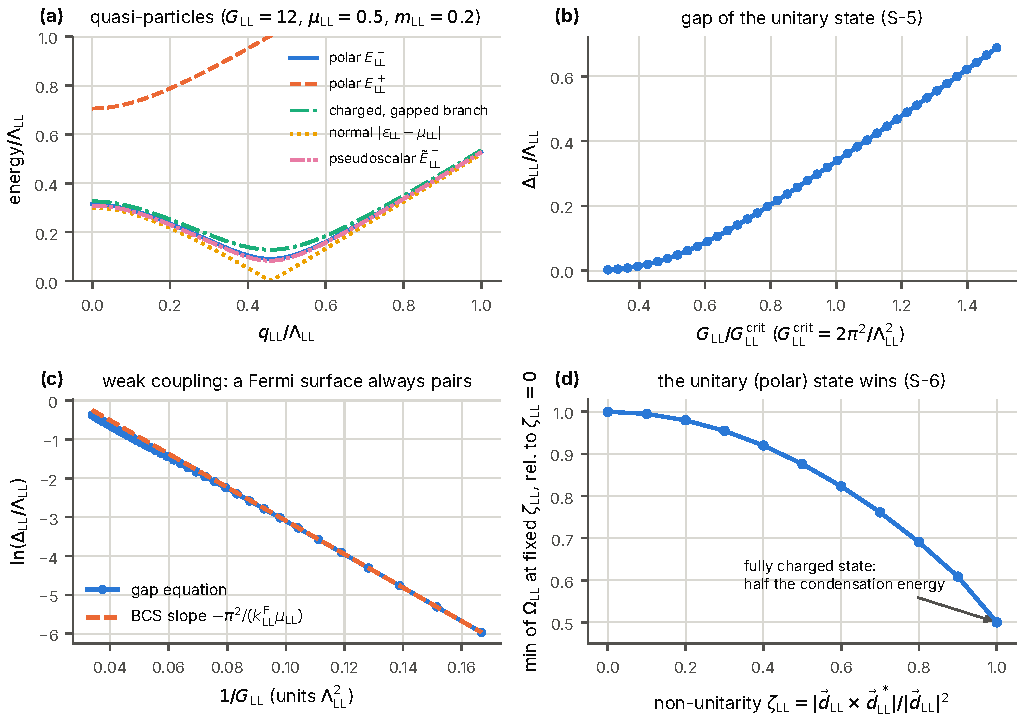
\includegraphics[width=\textwidth]{../figures/fig_sl_superfluid.pdf}
\caption{The spin-zero superfluid of the spinor charges ($\Lambda_{\rm LL}=1$). (a) Quasi-particle
energies versus momentum at $G_{\rm LL}=12$, $\mu_{\rm LL}=0.5$, $m_{\rm LL}=0.2$ (gap
$0.090417$): the polar state, the gapped branch of the charged state, the normal state and the
pseudoscalar channel at the same gap (Theorem SF2). (b) The gap of the unitary state versus the coupling
in units of $G^{\rm crit}_{\rm LL}$ at $m_{\rm LL}=0$, Eq.~(\ref{eq:gcrit}). (c) Weak coupling: $\ln\Delta_{\rm
LL}$ versus $1/G_{\rm LL}$ and the slope of Bardeen, Cooper and Schrieffer (S-5). (d) The minimum of
$\Omega_{\rm LL}$ at fixed non-unitarity $\zeta_{\rm LL}$, relative to the unitary state (Theorem SF3).}
\label{fig:superfluid}
\end{figure*}

\section{Are these theories renormalizable?}
\label{sec:renorm}

A quantum field theory is \emph{renormalizable} if the divergences of its perturbation theory can be
removed by adjusting finitely many parameters of its Lagrangian. The test is power counting. In
$D+1$ space-time dimensions (with $D$ the number of space dimensions) the action is dimensionless, so a
fermion field has the mass dimension $[\Psi_{\rm LL}]=D/2$, a scalar field $[\phi_{\rm LL}]=(D-1)/2$, and
the couplings have
\begin{equation}
[G_{\rm LL}]=1-D,\quad [g^{\rm Y}_{\rm LL}]=\tfrac{3-D}2,\quad [\lambda^{(1)}_{\rm LL}]=[\lambda^{(2)}_{\rm LL}]=3-D
\label{eq:dims}
\end{equation}
for the contact interaction of Eq.~(\ref{eq:ham}), a Yukawa coupling of a scalar to two fermions, and a
quartic coupling of scalars (R-1). A coupling of negative mass dimension makes a theory
non-renormalizable: for $D=3$ the contact coupling has $[G_{\rm LL}]=-2$, while the Yukawa and quartic
couplings are dimensionless; for $D=7$---the $7{+}1$ manifold, and the $4{+}4$ manifold, where power
counting sees the total dimension 8---all of them have negative dimension ($-6$, $-2$, $-4$).

\subsection{Power counting}

A one-particle-irreducible graph with $n^{\rm v}_{\rm LL}$ vertices, $n^{\rm int,F}_{\rm LL}$ internal
fermion and $n^{\rm int,B}_{\rm LL}$ internal boson lines has $n^{\rm loop}_{\rm LL}=n^{\rm int,F}_{\rm
LL}+n^{\rm int,B}_{\rm LL}-n^{\rm v}_{\rm LL}+1$ loops, and, since a fermion propagator falls like the
inverse momentum and a boson propagator like its square, the \emph{superficial degree of divergence}
\begin{equation}
\deg_{\rm LL}=(D+1)\,n^{\rm loop}_{\rm LL}-n^{\rm int,F}_{\rm LL}-2\,n^{\rm int,B}_{\rm LL}.
\label{eq:deg}
\end{equation}
Eliminating the internal lines with the number of line ends at the vertices gives, for the contact theory
and for the theory with Yukawa and quartic vertices,
\begin{align}
\deg_{\rm LL}&=(D+1)-\tfrac D2n^{\rm ext,F}_{\rm LL}+(D-1)\,n^{\rm v}_{\rm LL},\label{eq:degc}\\
\deg_{\rm LL}&=(D+1)-\tfrac D2n^{\rm ext,F}_{\rm LL}-\tfrac{D-1}2n^{\rm ext,B}_{\rm LL}\nonumber\\
&\quad+(D-3)\big(\tfrac12n^{\rm v,Y}_{\rm LL}+n^{\rm v,4}_{\rm LL}\big),\label{eq:degy}
\end{align}
with $n^{\rm ext,F}_{\rm LL}$, $n^{\rm ext,B}_{\rm LL}$ the external fermion and boson lines and
$n^{\rm v,Y}_{\rm LL}$, $n^{\rm v,4}_{\rm LL}$ the Yukawa and quartic vertices; check R-2 compares both
formulas with the direct count on all graphs with up to six vertices. For $D=3$ the degree of the
contact theory grows by 2 with every vertex: infinitely many counterterms are needed. The degree of the
Yukawa theory does not depend on the vertices: only the finitely many functions with $\deg_{\rm
LL}\ge0$ diverge. For $D=7$ both grow (Fig.~\ref{fig:renorm}(a)).

\subsection{The contact theory needs a cutoff}

At a fixed physical gap the bare coupling that solves the gap equation~(\ref{eq:gapeq}) must vary with
the cutoff as $G_{\rm LL}\Lambda_{\rm LL}^2/(2\pi^2)\to1$: the value is $0.99981$ at
$\Lambda_{\rm LL}=128$ ($\Delta_{\rm LL}=0.05$, $\mu_{\rm LL}=0.5$, $m_{\rm LL}=0.2$; R-3,
Fig.~\ref{fig:renorm}(b)). The cutoff cannot be removed by a finite number of logarithmic counterterms;
like the model of Nambu and Jona-Lasinio~\cite{NambuJonaLasinio1961}, the contact theory is an
effective theory valid below $\Lambda_{\rm LL}$.

\subsection{The Yukawa completion}

Replace the contact interaction by a complex isospin-triplet pair field $\phi_{\rm LL}=(\phi^1_{\rm
LL},\phi^2_{\rm LL},\phi^3_{\rm LL})$, a scalar of mass dimension 1 for $D=3$, with kinetic and mass
terms, the Yukawa coupling $g^{\rm Y}_{\rm LL}$ to the pairs $\Psi^T_{\rm LL}\mathsf K^\iota_{\rm LL}\Psi_{\rm
LL}$ (plus the Hermitian conjugate), and quartic self-couplings. Below the mass of $\phi_{\rm LL}$ its
exchange reproduces the contact interaction. The one-loop self-energy of $\phi_{\rm LL}$ is, up to the
constant factor of the traces over the Dirac and isospin indices, the Euclidean bubble
\begin{align}
I^{\rm bub}_{\rm LL}={}&\int_{k^{\rm E}_{\rm LL}<\Lambda_{\rm LL}}\!\frac{d^4k^{\rm E}_{\rm LL}}{(2\pi)^4}\nonumber\\
&\times\frac{k^{\rm E}_{\rm LL}\cdot(k^{\rm E}_{\rm LL}+p^{\rm E}_{\rm LL})+m_{\rm LL}^2}{[(k^{\rm E}_{\rm LL})^2+m_{\rm LL}^2][(k^{\rm E}_{\rm LL}+p^{\rm E}_{\rm LL})^2+m_{\rm LL}^2]}
\label{eq:bubble}
\end{align}
with the loop momentum $k^{\rm E}_{\rm LL}$ and the external momentum $p^{\rm E}_{\rm LL}$. Its value at
$p^{\rm E}_{\rm LL}=0$ grows like $\Lambda_{\rm LL}^2$ and is absorbed by the mass counterterm of
$\phi_{\rm LL}$; its momentum dependence grows like the logarithm of the cutoff, $d[I^{\rm bub}_{\rm
LL}(p^{\rm E}_{\rm LL})-I^{\rm bub}_{\rm LL}(0)]/d\ln\Lambda_{\rm LL}\to-(p^{\rm E}_{\rm LL})^2/(16\pi^2)$, and
is absorbed by the wave-function counterterm: the computed slope is $-6.332440\times10^{-3}$ against
$-6.332574\times10^{-3}$ (ratio $0.99998$; $p^{\rm E}_{\rm LL}=1$, $m_{\rm LL}=0.5$; R-4,
Fig.~\ref{fig:renorm}(c)). The list of renormalizable couplings is finite: besides $g^{\rm Y}_{\rm LL}$
and the masses, the quartic polynomials of $\phi_{\rm LL}$ invariant under isospin form a space of
dimension exactly 2, spanned by $(\phi^\dagger_{\rm LL}\phi_{\rm LL})^2$ and $\lvert\phi^T_{\rm
LL}\phi_{\rm LL}\rvert^2$ (R-5), with the couplings $\lambda^{(1)}_{\rm LL}$ and $\lambda^{(2)}_{\rm LL}$.

\subsection{Does non-associativity change the answer?}

No. A Lagrangian is built from fields on which the symmetry acts linearly, and a linear action of the
loop generates a Lie group (Sec.~\ref{sec:manifolds}). Check R-6 makes this precise for the simplest
case: the quadratic forms on $\mathbb B_{\rm LL}$ that are invariant under the 14 left multiplications
$L^{\rm LL}_{\mathbf x}$ and those invariant under their 56-dimensional Lie closure $\mathfrak{so}(8,\mathbb
C)$ form the same two-dimensional space, spanned by $\mathrm{Re}\,N_{\rm LL}$ and $\mathrm{Im}\,N_{\rm LL}$.
Every counterterm that the closure allows the loop allows, and conversely; power counting is unchanged.

\emph{Verdict.} In $3+1$ dimensions the spin-zero spinor superfluid of the super-loop is described by a
renormalizable theory in its Yukawa form; its contact form is non-renormalizable and needs the cutoff.
On the $7{+}1$ and $4{+}4$ manifolds every form is non-renormalizable. The non-associativity of the
super-loop neither causes nor cures this.

\begin{figure*}[t]
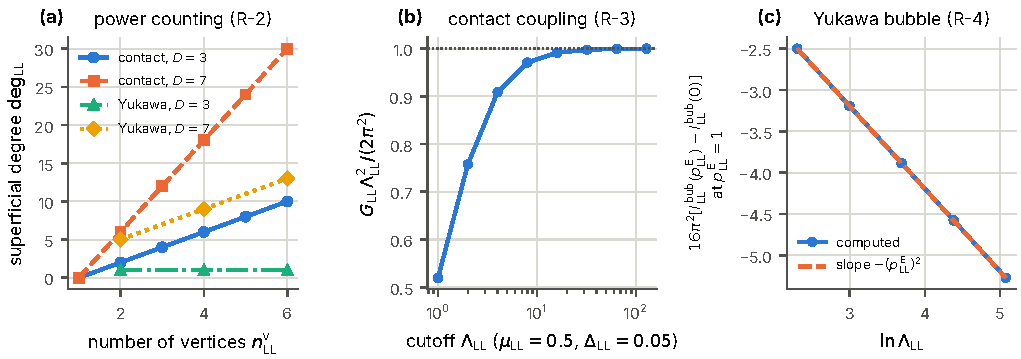
\includegraphics[width=\textwidth]{../figures/fig_sl_renorm.pdf}
\caption{Renormalizability. (a) The superficial degree of divergence of the four-fermion function of
the contact theory and of the fermion self-energy of the Yukawa theory versus the number of vertices,
Eqs.~(\ref{eq:degc}) and~(\ref{eq:degy}), for $D=3$ and $D=7$ (R-2). (b) The bare contact coupling at a
fixed gap versus the cutoff (R-3). (c) The momentum-dependent part of the bubble~(\ref{eq:bubble})
versus $\ln\Lambda_{\rm LL}$, with the slope $-(p^{\rm E}_{\rm LL})^2/(16\pi^2)$ (R-4).}
\label{fig:renorm}
\end{figure*}

\section{What has been established, and what has not}
\label{sec:status}

\subsection{Established}

\begin{itemize}
\item The algebraic facts of Secs.~\ref{sec:bioct} to~\ref{sec:operators}, in exact arithmetic: the
bi-octonions are alternative and not associative, their unit elements form a Moufang loop, and its
tangent algebra is a Malcev algebra that is not a Lie algebra; it contains $\mathfrak{so}(3,1)$ and eight
spinor charges with the quantum numbers of Fig.~\ref{fig:charges}.
\item Theorem R: the Malcev algebra has no non-zero realization by operators, and the loop is not a group
of operators.
\item Theorem L: no Lie algebra extends the Lorentz algebra by bosonic spinor charges whose brackets
contain Lorentz generators.
\item Theorem M: within the most general Lorentz- and isospin-covariant brackets on the sectors of the
families $\mathcal F^{\rm A}_{\rm LL}$, $\mathcal F^{\rm B}_{\rm LL}$, $\mathcal F^{\rm C}_{\rm LL}$, the
bi-octonion algebra is the unique Malcev algebra in which spinor charges close into Lorentz
generators. The necessary conditions are proved by ideal membership in Gr\"obner bases (every
polynomial used is a true consequence of the identity), and every solution is verified on all basis
tuples in exact arithmetic.
\item The manifolds of Sec.~\ref{sec:manifolds}, and the fact that the super-loop manifold is
parallelizable without a compatible Lie group structure.
\item The superfluid of Sec.~\ref{sec:superfluid} at the level of mean-field theory at zero temperature
with a sharp momentum cutoff: the channels (Theorem SF1), the spectra (SF2), the gap equation and its
critical coupling, the law of Bardeen, Cooper and Schrieffer, the ground state (SF3), its symmetry
breaking, and the super-loop singlet (SF4).
\item Power counting in $3+1$ and $7{+}1$ (and $4{+}4$) dimensions, the cutoff dependence of the contact
coupling, the divergence structure of the one-loop bubble of the Yukawa completion, the finite list of
its couplings, and the equality of loop invariance and closure invariance for quadratic forms.
\end{itemize}

\subsection{Not established}

\begin{itemize}
\item No quantum theory on a Hilbert space has the super-loop as a symmetry, and none can within
ordinary quantum mechanics (Theorem R). Whether a non-associative quantum mechanics, such as the
octonionic one of G\"unaydin, Piron and Ruegg~\cite{GunaydinPironRuegg1978}, can carry it was not
studied. The dynamical hypotheses H-dyn of the theorems on the scattering matrix are therefore not
tested.
\item The counterexample does not extend to the Poincar\'e algebra: with translations present no Malcev
algebra of our families lets spinor charges close into Lorentz generators (Theorem M(c)). Larger
families---more internal generators, central or tensorial charges, other representations of the
spinor charges---were not classified.
\item The field $\Psi_{\rm LL}$ of the superfluid is a fermion field by the spin-statistics theorem; it
carries the quantum numbers of the spinor charges, but the dynamics of Eq.~(\ref{eq:ham}) is an
ordinary relativistic field theory with the Lie symmetries $SL(2,\mathbb C)\times SU(2)_{\rm v}\times
U(1)^{\rm F}_{\rm LL}$, chosen by us. The name ``electric charge'' for $T^3_{\rm LL}$ is our choice (a
hypercharge could be added).
\item The superfluid was not treated beyond mean field: no fluctuation corrections, no finite
temperature, no dispersion of the Goldstone modes, no other interactions.
\item Renormalizability is decided by power counting and by the one-loop divergence structure of the
Yukawa completion, not by a renormalization to all orders.
\end{itemize}

\section{Conclusions}
\label{sec:conclusions}

Every proof of the no-go theorems treats symmetries as associative objects: a group, operators on a
space of states, generators with a Jacobi identity. Dropping associativity, and only that, the unit
bi-octonions give a structure in which the Lorentz group and internal charges are united: the Lorentz
super-loop $\mathbb L_{\rm LL}$, a Moufang loop that contains $SL(2,\mathbb C)$ and eight spinor charges, a
Weyl spinor that is an isospin doublet with electric charges $\pm\tfrac12$, whose brackets close into
the Lorentz generators. No Lie algebra can do this (Theorem L); among all covariant brackets the
super-loop is the only Malcev algebra that does (Theorem M); and its non-associativity is essential,
because it has no realization by operators (Theorem R). The super-loop carries operators with the
eigenvalues of electric charge, isospin, spin, chirality and spinor number, and a new one, the twist
charge, whose value $-2$ on the spinor charges measures how far the Lorentz action on them is from a
representation. It realizes the inversion of the Lorentz group as an element, which no group can. It
lives on the $7{+}1$ and $3+1$ Minkowski spaces inside the bi-octonions, on the $4{+}4$ split octonions, and
on itself, a parallelizable manifold without a group structure. The spin-zero superfluid of its spinor
charges condenses in an isospin-triplet, unitary, electrically neutral state, and the pair that is a
singlet of the whole super-loop requires two species. In $3+1$ dimensions its Yukawa form is
renormalizable; on the eight-dimensional manifolds it is not.

\section*{Data Availability}

The data that support the findings of this article are openly available in the repository of PROJECT
spacetimes, folder \texttt{Revision\_SuperLoop}, at \url{https://github.com/once-ere/spacetimes}: the
programs, every data file, the reports of all machine checks, the figures and the sources of this paper
(Appendix~\ref{app:data}).

\appendix
\onecolumngrid

\section{Notation}
\label{app:notation}

Table~\ref{tab:symbols} defines every symbol of this paper, by group, with the plain-text names under
which the programs, the figures and the data files write it. Two entries are taken from the master
registries of the symbols of PROJECT spacetimes and keep exactly the meaning that they have in the
rest of the project, followed by a note on their use here: the index $j$ (registered in the project as
$i,j$, the index of the space-like coordinates; here only $j$ is an index, and $i$ is the imaginary
unit) and the number $D$ of space dimensions. All other entries are new. Every new symbol carries the
suffix LL (for \emph{Lorentz super-loop}), written as a subscript ($Q_{\rm LL}$) or, where the lower
position holds an index, as a superscript ($\sigma^{\rm LL}_j$), except the following, which cannot be
read as anything else: the bi-octonions and their parts in bold upright type ($\mathbf x$, $\mathbf
e_p$, $\mathbf u$, $\mathbf b$, \dots), the unit matrix $\mathsf 1_4$ and the operators $\mathsf O_1$,
$\mathsf O_2$, $\mathsf O_3$ of Sec.~\ref{sec:nogo}, the number sets and algebras in blackboard type
($\mathbb R$, $\mathbb C$, $\mathbb H$, $\mathbb O$), the groups and Lie algebras ($SL(2,\mathbb C)$,
$\mathfrak{so}(3,1)$, \dots), operation signs, and the plain symbols $i$ (the imaginary unit), $p$ (an
index over the basis of an algebra) and $\iota$ (the isospin index). The letter $\mathsf K$ without
scripts in Theorem~SF1 is any $8\times8$ pair matrix.

The machine checks LL-S1 to LL-S8 (Appendix~\ref{app:checks}) verify that the symbols obey these rules:
no symbol and no plain-text name is registered twice (LL-S1); the taken entries carry the meanings of
the master registries, no new symbol coincides with a symbol of a master registry, and the symbols that
this paper shares with the sibling folder \texttt{Revision\_NoGo} of the repository are declared and
denote the same objects there (LL-S2); every column of every data file is a registered name or a
descriptive word (LL-S3); every document of this revision contains the complete table of symbols
(LL-S4); the symbols of the superfluid, $\mu_{\rm LL}$, $\Lambda_{\rm LL}$, $\Omega_{\rm LL}$,
$\nu^{\rm F}_{\rm LL}$, $\Delta_{\rm LL}$, $\zeta_{\rm LL}$, $\varepsilon_{\rm LL}$, always carry their suffix
(LL-S5); no letter that the project uses with another meaning occurs in a formula without the suffix
LL (LL-S6); every letter in bold, sans-serif, calligraphic, blackboard or fraktur type is registered
(LL-S7); and every name with the suffix \texttt{\_LL}, every name of an algebra element, every
coefficient and every pair matrix that occurs in a report or data file is registered (LL-S8). Units:
$\hbar$ and the speed of light are 1; in Secs.~\ref{sec:superfluid} and~\ref{sec:renorm} the momentum
cutoff $\Lambda_{\rm LL}=1$ unless a unit is shown.

{\small\longtabledepth
\begin{longtable}{p{0.24\textwidth}p{0.54\textwidth}>{\raggedright\arraybackslash\footnotesize}p{0.16\textwidth}}
\caption{The symbols of this paper, by group, with the plain-text names under which the programs, the
figures and the data files write them.}\label{tab:symbols}\\
\toprule
symbol & meaning & plain-text names\\
\midrule
\endfirsthead
\toprule
symbol & meaning (continued) & plain-text names\\
\midrule
\endhead
\bottomrule
\endfoot
\multicolumn{3}{l}{\textbf{1 Indices, conventions and number sets}}\\
$i,j$ & index of space-like coordinates; values 1, 2, 3 (ordinary space) unless a sum is said to run over all space-like coordinates of the spacetime. In Revision\_SuperLoop only $j$ is used as an index, with the values 1, 2, 3, and with primes ($j'$, $j''$) where two or three such indices are needed: it labels the three imaginary quaternion units $\mathbf e_j$, which correspond to the three space directions of $\mathbb R^{1,3}_{\rm LL}$, the coordinates $x^j_{\rm LL}$, the momentum components $q^j_{\rm LL}$, the rotation and boost generators $J^j_{\rm LL}$, $K^j_{\rm LL}$, and the Pauli matrices $\sigma^{\rm LL}_j$ and Dirac matrices $\alpha^j_{\rm LL}$, $\gamma^j_{\rm LL}$. The letter $i$ is the imaginary unit (entry $i$); the isospin index is $\iota$ (a different letter). & \texttt{j} \texttt{j'} \texttt{j''}\\
$D$ & the number of space dimensions in which the particles of matter have momentum: 7 (all space coordinates of 7+1), 4 (fields that do not depend on $x5,x6,x7$) or 3 (fields that depend on ordinary space only). $V_D=\pi^{D/2}/\Gamma_{\rm E}(D/2+1)$ is the volume and $A_D=D\,V_D$ the area of the unit ball in $D$ dimensions ($\Gamma_{\rm E}$: Euler's gamma function). In Revision\_SuperLoop $D=3$ for the four-dimensional world of the superfluid and $D=7$ for the eight-dimensional manifolds (on $4{+}4$ power counting sees the total dimension 8 as well); the value 4, the coordinates $x5,x6,x7$ of the eight-dimensional spacetime of the project (on which such fields do not depend), and the volume and the area of the unit ball do not occur. & \texttt{D}\\
$i$ & the imaginary unit, $i^2=-1$; in $\mathbb B_{\rm LL}$ it is the imaginary unit of the complex coefficients: it commutes and associates with every bi-octonion and is not one of the units $\mathbf e_1,\dots,\mathbf e_7$ & \\
$\mathbb R$, $\mathbb C$ & the real and the complex numbers (plain text: \texttt{R\^{}8}, \texttt{C\^{}3}, \texttt{C\^{}8} are the real or complex vector spaces of that dimension) & \texttt{R} \texttt{C} \texttt{R\^{}8} \texttt{C\^{}3} \texttt{C\^{}8}\\
$p$, $p'$ & a summation index over the basis of an algebra (values $0,\dots,7$, or $0,\dots,3$ for the quaternions): in Revision\_SuperLoop it labels the units $\mathbf e_p$ of $\mathbb B_{\rm LL}$, the coefficients $\xi^{\rm LL}_p(\mathbf x)$, the coordinates $x^p_{\rm LL}$ of $\mathbb R^{1,7}_{\rm LL}$ and $\mathbb R^{1,3}_{\rm LL}$ and the Dirac matrices $\gamma^p_{\rm LL}$ ($p=0,1,2,3$); $p'$ is a second index of the same kind (plain text \texttt{p1}, \texttt{p2}, \texttt{p3}: three such indices) & \texttt{p} \texttt{p'} \texttt{p1} \texttt{p2} \texttt{p3}\\
$\iota$, $\iota'$, $\iota''$ & the isospin index, values 1, 2, 3: it labels the isospin generators $T^\iota_{\rm LL}$, the Pauli matrices $\tau^{\rm LL}_\iota$ on the isospin index of a field, the pair channels $\mathsf K^\iota_{\rm LL}$, $\mathsf K'^\iota_{\rm LL}$, the pair operators $\Pi^\iota_{\rm LL}$ and the components $d^\iota_{\rm LL}$ of the order parameter; it is an internal direction, not a direction in space (that is $j$) & \texttt{iota}\\
$\epsilon^{\rm LL}_{jj'j''}$ & the Levi-Civita symbol: $+1$ if $(j,j',j'')$ is an even permutation of $(1,2,3)$, $-1$ if it is an odd one, $0$ otherwise; also with the isospin indices, $\epsilon^{\rm LL}_{\iota\iota'\iota''}$ & \texttt{eps3}\\
$\sigma^{\rm LL}_0$, $\sigma^{\rm LL}_j$ & the $2\times2$ unit matrix $\sigma^{\rm LL}_0$ and the Pauli matrices $\sigma^{\rm LL}_1=\begin{pmatrix}0&1\\1&0\end{pmatrix}$, $\sigma^{\rm LL}_2=\begin{pmatrix}0&-i\\i&0\end{pmatrix}$, $\sigma^{\rm LL}_3=\begin{pmatrix}1&0\\0&-1\end{pmatrix}$, acting on the two components of a Weyl spinor or on the species index & \texttt{sigma\_0} \texttt{sigma\_j} \texttt{sigma\_1} \texttt{sigma\_2} \texttt{sigma\_3}\\
$\tau^{\rm LL}_\iota$ & the same three Pauli matrices acting on the isospin index of a field (the index of the two components up and down of an isodoublet) & \texttt{tau\_iota} \texttt{tau\_1} \texttt{tau\_2} \texttt{tau\_3}\\
$\mathsf E_{\rm LL}$ & the real antisymmetric $2\times2$ matrix $i\sigma^{\rm LL}_2=\begin{pmatrix}0&1\\-1&0\end{pmatrix}$, with $\mathsf E_{\rm LL}^{-1}=\mathsf E_{\rm LL}^T=-\mathsf E_{\rm LL}$; it acts on a Weyl, isospin or species index, as stated at each place & \texttt{eps2}\\
$\mathsf 1_4$, $\mathsf 1_8$ & the $4\times4$ and the $8\times8$ unit matrices & \\
\multicolumn{3}{l}{\textbf{2 The bi-octonions and the super-loop}}\\
$\mathbb H$, $\mathbb O$ & the quaternions and the octonions: the real combinations of $\mathbf e_0,\dots,\mathbf e_3$ and of $\mathbf e_0,\dots,\mathbf e_7$; ${\rm Im}\,\mathbb H$ and ${\rm Im}\,\mathbb O$ are their imaginary parts, the real combinations of $\mathbf e_1,\mathbf e_2,\mathbf e_3$ and of $\mathbf e_1,\dots,\mathbf e_7$ (plain text \texttt{Im H}, \texttt{Im O}; \texttt{C (x) H} is $\mathbb C\otimes\mathbb H$, the bi-quaternions) & \texttt{H} \texttt{O}\\
$\mathbb B_{\rm LL}$ & the bi-octonions $\mathbb C\otimes\mathbb O$: the complex combinations $\mathbf x=\sum_{p=0}^7\xi^{\rm LL}_p(\mathbf x)\,\mathbf e_p$ of the eight units, with the product of the units extended bilinearly; real dimension 16 & \texttt{B\_LL}\\
$\mathbf e_0,\dots,\mathbf e_7$; $\mathbf e_p$, $\mathbf e_j$, $\mathbf e_\iota$ & the units of $\mathbb B_{\rm LL}$, of $\mathbb O$ and of $\mathbb H$: $\mathbf e_0=1$; $\mathbf e_1,\mathbf e_2,\mathbf e_3$ the quaternion units, $\mathbf e_j^2=-1$, $\mathbf e_1\mathbf e_2=-\mathbf e_2\mathbf e_1=\mathbf e_3$ and cyclically; $\mathbf e_4$ the unit of the Cayley-Dickson doubling, $\mathbf e_4^2=-1$; $\mathbf e_5=\mathbf e_1\mathbf e_4$, $\mathbf e_6=\mathbf e_2\mathbf e_4$, $\mathbf e_7=\mathbf e_3\mathbf e_4$ ($\mathbf e_\iota$: a quaternion unit labelled by the isospin index; plain text \texttt{ie1}, ..., \texttt{ie7}: the bi-octonions $i\mathbf e_1,\dots,i\mathbf e_7$) & \texttt{e0} \texttt{e1} \texttt{e2} \texttt{e3} \texttt{e4} \texttt{e5} \texttt{e6} \texttt{e7} \texttt{e\_p} \texttt{e\_p'} \texttt{e\_j} \texttt{e\_iota} \texttt{e\_p1} \texttt{e\_p2} \texttt{e\_p3} \texttt{ie1} \texttt{ie2} \texttt{ie3} \texttt{ie4} \texttt{ie5} \texttt{ie6} \texttt{ie7}\\
$\xi^{\rm LL}_p(\mathbf x)$ & the complex coefficient of the unit $\mathbf e_p$ in the bi-octonion $\mathbf x$ & \texttt{xi\_p} \texttt{xi\_0} \texttt{xi\_1} \texttt{xi\_2} \texttt{xi\_3}\\
$\mathbf x$, $\mathbf y$, $\mathbf z$, $\mathbf w$ & elements of $\mathbb B_{\rm LL}$ (bi-octonions); $\mathbf w$ is also a point of the super-loop manifold $\mathbb L_{\rm LL}$ & \texttt{x} \texttt{y} \texttt{z} \texttt{w}\\
$\mathbf a$, $\mathbf b$, $\mathbf c$, $\mathbf d$; $\mathbf b'$ & bi-quaternions: elements of $\mathbb C\otimes\mathbb H$, the complex combinations of $\mathbf e_0,\mathbf e_1,\mathbf e_2,\mathbf e_3$; every bi-octonion is written $\mathbf x=\mathbf a+\mathbf b\,\mathbf e_4$ (Cayley-Dickson form), and $\mathbf b\,\mathbf e_4$, $\mathbf b'\,\mathbf e_4$ are spinor charges & \texttt{aH} \texttt{bS} \texttt{cH} \texttt{dS} \texttt{bS'}\\
$\bar{\mathbf x}$, $\mathbf x^*$, $\mathbf x^\dagger$ & the three conjugations (also of bi-quaternions): $\bar{\mathbf x}$ changes the signs of the coefficients of $\mathbf e_1,\dots,\mathbf e_7$ (it is complex-linear, $\overline{\mathbf x\mathbf y}=\bar{\mathbf y}\,\bar{\mathbf x}$, and $\overline{\mathbf a+\mathbf b\mathbf e_4}=\bar{\mathbf a}-\mathbf b\mathbf e_4$); $\mathbf x^*$ replaces every complex coefficient by its complex conjugate; $\mathbf x^\dagger=(\bar{\mathbf x})^*$ (plain text: \texttt{xbar}, \texttt{x\^{}*}, \texttt{x\^{}dag}, and likewise \texttt{aHbar}, \texttt{gL\^{}dag}, ...) & \texttt{xbar} \texttt{x\^{}*} \texttt{x\^{}dag} \texttt{aHbar} \texttt{bSbar} \texttt{bS'bar} \texttt{cHbar} \texttt{dSbar} \texttt{gLbar} \texttt{hLbar} \texttt{rPbar} \texttt{rP'bar} \texttt{bS\^{}*} \texttt{bS'\^{}*} \texttt{gL\^{}*} \texttt{gL\^{}dag} \texttt{uL\^{}dag}\\
$N_{\rm LL}(\mathbf x)$, $N_{\rm LL}(\mathbf x,\mathbf y)$ & the complex norm $N_{\rm LL}(\mathbf x)=\sum_p\xi^{\rm LL}_p(\mathbf x)^2$, with $\mathbf x\bar{\mathbf x}=\bar{\mathbf x}\mathbf x=N_{\rm LL}(\mathbf x)\,\mathbf e_0$, and its polarization $N_{\rm LL}(\mathbf x,\mathbf y)=\sum_p\xi^{\rm LL}_p(\mathbf x)\,\xi^{\rm LL}_p(\mathbf y)$, $N_{\rm LL}(\mathbf x,\mathbf x)=N_{\rm LL}(\mathbf x)$ (complex-valued; for bi-quaternions the determinant of the $2\times2$ matrix $M_{\rm LL}$) & \texttt{N\_LL}\\
$[\mathbf x,\mathbf y]$; $[\mathbf x,\mathbf y,\mathbf z]$ & the commutator $\mathbf x\mathbf y-\mathbf y\mathbf x$ and the associator $(\mathbf x\mathbf y)\mathbf z-\mathbf x(\mathbf y\mathbf z)$ of bi-octonions (the same brackets of other elements are defined at their place: the bracket of an algebra $\mathcal F^{\rm A}_{\rm LL}$, $\mathcal F^{\rm B}_{\rm LL}$, $\mathcal F^{\rm C}_{\rm LL}$, and the commutator of two matrices or operators, the product in one order minus the product in the other) & \texttt{[x,y]} \texttt{[x,y,z]}\\
$\mathrm{Jac}_{\rm LL}$ & the Jacobiator $\mathrm{Jac}_{\rm LL}(\mathbf x,\mathbf y,\mathbf z)=[[\mathbf x,\mathbf y],\mathbf z]+[[\mathbf y,\mathbf z],\mathbf x]+[[\mathbf z,\mathbf x],\mathbf y]$ of a bracket; it vanishes identically exactly in a Lie algebra & \texttt{Jac}\\
$L^{\rm LL}_{\mathbf x}$, $R^{\rm LL}_{\mathbf x}$ & the left and right multiplications $\mathbf y\mapsto\mathbf x\mathbf y$ and $\mathbf y\mapsto\mathbf y\mathbf x$ by a bi-octonion, real $16\times16$ matrices (on $\mathbb O$ or $\mathbb O^{\rm s}_{\rm LL}$: $8\times8$) & \texttt{L\_x} \texttt{L\_y} \texttt{L\_e1} \texttt{L\_e4} \texttt{L\_[e1,e4]} \texttt{L\_(e\_p)} \texttt{L\_(e\_p')} \texttt{R\_x} \texttt{R\_y}\\
$\mathbb L_{\rm LL}$ & the Lorentz super-loop: the unit bi-octonions, $\mathbb L_{\rm LL}=\{\mathbf w\in\mathbb B_{\rm LL}:N_{\rm LL}(\mathbf w)=1\}$, with the product of $\mathbb B_{\rm LL}$; a Moufang loop (not a group), and a manifold of real dimension 14 & \texttt{L\_LL}\\
$\mathbf g$, $\mathbf h$ & elements of $SL(2,\mathbb C)$, i.e. unit bi-quaternions ($N_{\rm LL}(\mathbf g)=1$), a subgroup of $\mathbb L_{\rm LL}$ & \texttt{gL} \texttt{hL}\\
$\mathbf v$ & a unit (bi-)quaternion that rotates the isospin of the spinor charges (from the left) & \texttt{vI}\\
$\mathfrak m_{\rm LL}$, $\mathfrak l_{\rm LL}$, $\mathfrak s_{\rm LL}$ & the Malcev algebra of the super-loop, $\mathfrak m_{\rm LL}=\mathbb C\otimes{\rm Im}\,\mathbb O$ with the commutator (real dimension 14), its Lorentz part $\mathfrak l_{\rm LL}=\mathbb C\otimes{\rm Im}\,\mathbb H$ (6, a Lie algebra isomorphic to $\mathfrak{so}(3,1)$), and the space of spinor charges $\mathfrak s_{\rm LL}=(\mathbb C\otimes\mathbb H)\,\mathbf e_4$ (8); $\mathfrak m_{\rm LL}=\mathfrak l_{\rm LL}\oplus\mathfrak s_{\rm LL}$ & \texttt{m\_LL} \texttt{l\_LL} \texttt{s\_LL}\\
$J^j_{\rm LL}$, $K^j_{\rm LL}$ & the rotation and boost generators of $\mathfrak l_{\rm LL}$, $J^j_{\rm LL}=\mathbf e_j/2$ and $K^j_{\rm LL}=i\,\mathbf e_j/2$ & \texttt{J\_LL\^{}j} \texttt{K\_LL\^{}j} \texttt{J\_LL\^{}j'} \texttt{K\_LL\^{}j'} \texttt{J\_LL\^{}j''} \texttt{K\_LL\^{}j''} \texttt{J\_LL\^{}3}\\
$\mathbf u$, $\mathbf u'$, $\mathbf u_1$, $\mathbf u_2$ & elements of the Lorentz part $\mathfrak l_{\rm LL}$ (Lorentz generators): imaginary bi-quaternions & \texttt{uL} \texttt{uL'} \texttt{uL1} \texttt{uL2}\\
$\mathbf t$, $\mathbf t'$ & elements of ${\rm Im}\,\mathbb H$ (real imaginary quaternions): isospin generators, which act on the spinor charges from the left & \texttt{tI} \texttt{tI'}\\
$W_{\rm LL}(\mathbf u)$ & the Weyl representation of $\mathfrak l_{\rm LL}$ on bi-quaternions, $W_{\rm LL}(\mathbf u)\mathbf b=-\mathbf b\,\mathbf u$: a Lie representation, $[W_{\rm LL}(\mathbf u_1),W_{\rm LL}(\mathbf u_2)]=W_{\rm LL}([\mathbf u_1,\mathbf u_2])$ & \texttt{W\_LL}\\
$\rho_{\rm LL}(\mathbf u)$ & the inner action of a Lorentz element on the spinor charges, $[\mathbf u,\mathbf b\,\mathbf e_4]=(\rho_{\rm LL}(\mathbf u)\mathbf b)\,\mathbf e_4$ with $\rho_{\rm LL}=-2W_{\rm LL}$; not a representation & \texttt{rho\_LL}\\
$\Theta_{\rm LL}$ & the twist charge: the linear map of $\mathfrak m_{\rm LL}$ that is $1$ on $\mathfrak l_{\rm LL}$ and $-2$ on $\mathfrak s_{\rm LL}$; the inner action is $[\mathbf u,\cdot\,]=D_{\rm LL}(\mathbf u)\circ\Theta_{\rm LL}$ (as a number: the eigenvalue $1$ or $-2$, or the value of $c^{\rm tw}_{\rm LL}$ in the families) & \texttt{Theta\_LL} \texttt{Theta\_LL\^{}2}\\
$D_{\rm LL}(\mathbf u)$, $D^{\rm v}_{\rm LL}(\mathbf t)$ & the Lorentz and isospin derivations of $\mathbb B_{\rm LL}$: $D_{\rm LL}(\mathbf u)(\mathbf a+\mathbf b\mathbf e_4)=[\mathbf u,\mathbf a]+(-\mathbf b\mathbf u)\mathbf e_4$ and $D^{\rm v}_{\rm LL}(\mathbf t)(\mathbf a+\mathbf b\mathbf e_4)=(\mathbf t\mathbf b)\mathbf e_4$ (both linear in their argument) & \texttt{D\_LL} \texttt{Dv\_LL}\\
$\mathcal D_{\rm LL}$ & a derivation of $\mathbb B_{\rm LL}$: a linear map with $\mathcal D_{\rm LL}(\mathbf x\mathbf y)=(\mathcal D_{\rm LL}\mathbf x)\mathbf y+\mathbf x(\mathcal D_{\rm LL}\mathbf y)$, the infinitesimal form of an automorphism & \\
$\varphi^{\rm LL}_{\mathbf g,\mathbf v}$ & the automorphism $\mathbf a+\mathbf b\mathbf e_4\mapsto\mathbf g\mathbf a\bar{\mathbf g}+(\mathbf v\mathbf b\bar{\mathbf g})\mathbf e_4$ of $\mathbb B_{\rm LL}$ ($\mathbf g$ a Lorentz transformation, $\mathbf v$ an isospin rotation) & \texttt{varphi}\\
$\varrho_{\rm LL}$; $\mathsf O_1$, $\mathsf O_2$, $\mathsf O_3$ & a linear map from $\mathfrak m_{\rm LL}$ to the linear operators (matrices) on a vector space that turns brackets into commutators, $\varrho_{\rm LL}([\mathbf x,\mathbf y])=\varrho_{\rm LL}(\mathbf x)\varrho_{\rm LL}(\mathbf y)-\varrho_{\rm LL}(\mathbf y)\varrho_{\rm LL}(\mathbf x)$ (Theorem R); $\mathsf O_1,\mathsf O_2,\mathsf O_3$ three such operators & \\
$\mathrm{Kil}_{\rm LL}$; $\mathrm{ad}$ & the Killing form $\mathrm{Kil}_{\rm LL}(\mathbf x,\mathbf y)=\mathrm{tr}(\mathrm{ad}\,\mathbf x\,\mathrm{ad}\,\mathbf y)$ of a Lie algebra, where $\mathrm{ad}\,\mathbf x$ is the matrix of the map $\mathbf y\mapsto[\mathbf x,\mathbf y]$ & \texttt{Killing} \texttt{ad}\\
\multicolumn{3}{l}{\textbf{3 Operators on the super-loop and their eigenvalues}}\\
$Q_{\rm LL}$ & the electric charge, $Q_{\rm LL}=T^3_{\rm LL}$: eigenvalues $0$ on $\mathbb C\otimes\mathbb H$ and $\pm\tfrac12$ on the spinor charges & \texttt{Q\_LL}\\
$T^\iota_{\rm LL}$, $(T_{\rm LL})^2$ & the isospin generators $T^\iota_{\rm LL}=i\,D^{\rm v}_{\rm LL}(\mathbf e_\iota/2)$, Hermitian, $[T^1_{\rm LL},T^2_{\rm LL}]=iT^3_{\rm LL}$ and cyclically, and the isospin Casimir $(T_{\rm LL})^2=\sum_\iota(T^\iota_{\rm LL})^2$ & \texttt{T\_LL\^{}iota} \texttt{T\_LL\^{}iota'} \texttt{T\_LL\^{}iota''} \texttt{T\_LL\^{}3} \texttt{T\_LL\^{}2}\\
$\mathrm{Cas}_{\rm LL}$ & the Casimir operator of the rotations, $\mathrm{Cas}_{\rm LL}=-\sum_jD_{\rm LL}(J^j_{\rm LL})^2$; its eigenvalue is 0 for spin 0, 3/4 for spin 1/2 and 2 for spin 1 & \texttt{Cas\_LL}\\
\multicolumn{3}{l}{\textbf{4 The covariant families and their classification}}\\
$\mathcal F^{\rm A}_{\rm LL}$, $\mathcal F^{\rm B}_{\rm LL}$, $\mathcal F^{\rm C}_{\rm LL}$ & the three families of covariant brackets: $\mathcal F^{\rm A}_{\rm LL}$ on $\mathfrak l_{\rm LL}\oplus\mathfrak s_{\rm LL}$ (dimension 14), $\mathcal F^{\rm B}_{\rm LL}$ on $\mathfrak l_{\rm LL}\oplus\mathfrak p_{\rm LL}\oplus\mathfrak s_{\rm LL}$ (18), $\mathcal F^{\rm C}_{\rm LL}$ on $\mathfrak l_{\rm LL}\oplus\mathfrak{su}(2)\oplus\mathfrak s_{\rm LL}$ (17) & \texttt{F\_A} \texttt{F\_B} \texttt{F\_C}\\
$\mathfrak p_{\rm LL}$; $\mathbf r$, $\mathbf r'$ & the translations of the family $\mathcal F^{\rm B}_{\rm LL}$: the real space of the Hermitian bi-quaternions $\mathbf r=\mathbf r^\dagger$ (dimension 4), on which $\mathfrak l_{\rm LL}$ acts by $[\mathbf u,\mathbf r]=\mathbf u\mathbf r+\mathbf r\mathbf u^\dagger$ & \texttt{p\_LL} \texttt{rP} \texttt{rP'}\\
$c^{\rm tw}_{\rm LL}$, $c^{\rm sl}_{\rm LL}$, $c^{\rm PP}_{\rm LL}$, $c^{\rm Ps}_{\rm LL}$, $c^{\rm sP}_{\rm LL}$, $c^{\rm TT}_{\rm LL}$, $c^{\rm Ts}_{\rm LL}$, $c^{\rm sT}_{\rm LL}$ & the coefficients of the families: $[\mathbf u,\mathbf b\mathbf e_4]=c^{\rm tw}_{\rm LL}(W_{\rm LL}(\mathbf u)\mathbf b)\mathbf e_4$ (the twist), $[\mathbf b\mathbf e_4,\mathbf b'\mathbf e_4]\supset c^{\rm sl}_{\rm LL}(\bar{\mathbf b}\mathbf b'-\bar{\mathbf b}'\mathbf b)$, $[\mathbf r,\mathbf r']=c^{\rm PP}_{\rm LL}(\mathbf r\bar{\mathbf r}'-\mathbf r'\bar{\mathbf r})$, $[\mathbf r,\mathbf b\mathbf e_4]=c^{\rm Ps}_{\rm LL}(\mathbf b^*\bar{\mathbf r})\mathbf e_4$, $[\mathbf b\mathbf e_4,\mathbf b'\mathbf e_4]\supset c^{\rm sP}_{\rm LL}\,i(\bar{\mathbf b}\mathbf b'^*-\bar{\mathbf b}'\mathbf b^*)$, $[\mathbf t,\mathbf t']=c^{\rm TT}_{\rm LL}(\mathbf t\mathbf t'-\mathbf t'\mathbf t)$, $[\mathbf t,\mathbf b\mathbf e_4]=c^{\rm Ts}_{\rm LL}(\mathbf t\mathbf b)\mathbf e_4$, $[\mathbf b\mathbf e_4,\mathbf b'\mathbf e_4]\supset\mathrm{Re}[c^{\rm sT}_{\rm LL}(\mathbf b\bar{\mathbf b}'-\mathbf b'\bar{\mathbf b})]$; complex except $c^{\rm sP}_{\rm LL}$, $c^{\rm TT}_{\rm LL}$ (real); plain text \texttt{ctw\_re}, \texttt{ctw\_im}: real and imaginary part of $c^{\rm tw}_{\rm LL}$, and likewise & \texttt{c\_tw} \texttt{c\_sl} \texttt{c\_PP} \texttt{c\_Ps} \texttt{c\_sP} \texttt{c\_TT} \texttt{c\_Ts} \texttt{c\_sT} \texttt{csP} \texttt{cTT} \texttt{ctw\_re} \texttt{ctw\_im} \texttt{csl\_re} \texttt{csl\_im} \texttt{cPP\_re} \texttt{cPP\_im} \texttt{cPs\_re} \texttt{cPs\_im} \texttt{cTs\_re} \texttt{cTs\_im} \texttt{csT\_re} \texttt{csT\_im}\\
$\lambda^{\rm sc}_{\rm LL}$ & a complex number $\neq0$ by which the spinor charges are rescaled, $\mathbf b\mapsto\lambda^{\rm sc}_{\rm LL}\mathbf b$ & \texttt{lambda\_sc}\\
$\mathcal I^{\rm Jac}_{\rm LL}$, $\mathcal I^{\rm Mal}_{\rm LL}$; $w^{\rm sat}_{\rm LL}$ & the ideals of polynomials in the real coefficients of a family generated by the Jacobi and by the Malcev identity; $w^{\rm sat}_{\rm LL}$ the auxiliary variable of the saturation (the points of the variety at which a given polynomial does not vanish are the points of the variety of the ideal enlarged by that polynomial times $w^{\rm sat}_{\rm LL}$, minus 1) & \texttt{w\_sat}\\
\multicolumn{3}{l}{\textbf{5 The manifolds}}\\
$\mathbb R^{1,7}_{\rm LL}$, $\mathbb R^{1,3}_{\rm LL}$; $x^p_{\rm LL}$ & the Hermitian bi-octonions $\mathbf x=\mathbf x^\dagger=x^0_{\rm LL}\mathbf e_0+i\sum_{p=1}^7x^p_{\rm LL}\mathbf e_p$ (real $x^p_{\rm LL}$): the $7{+}1$ Minkowski space with the real norm $N_{\rm LL}(\mathbf x)=(x^0_{\rm LL})^2-\sum_p(x^p_{\rm LL})^2$; and its subspace of Hermitian bi-quaternions ($p\le3$), Minkowski space of $3+1$ dimensions & \texttt{R\^{}(1,7)\_LL} \texttt{R\^{}(1,3)\_LL} \texttt{x\_LL\^{}0} \texttt{x\_LL\^{}p} \texttt{x\_LL\^{}1} \texttt{x\_LL\^{}2} \texttt{x\_LL\^{}3} \texttt{x\_LL\^{}j}\\
$\mathbb O^{\rm s}_{\rm LL}$ & the split octonions inside $\mathbb B_{\rm LL}$: the real space $\mathbb H+(i\mathbb H)\mathbf e_4$ (real combinations of $\mathbf e_0,\dots,\mathbf e_3,i\mathbf e_4,\dots,i\mathbf e_7$), closed under the product, on which $N_{\rm LL}$ has signature $(4,4)$: the $4{+}4$ manifold (plain text \texttt{R\^{}(4,4)}) & \texttt{Os} \texttt{R\^{}(4,4)}\\
$S^7_{\rm LL}$, $S^{3,4}_{\rm LL}$ & the unit elements ($N_{\rm LL}=1$) of $\mathbb O$ (the seven-sphere) and of $\mathbb O^{\rm s}_{\rm LL}$ (the pseudo-sphere): the two real forms of $\mathbb L_{\rm LL}$, both Moufang loops & \texttt{S\^{}7} \texttt{S\^{}(3,4)}\\
$X^{\rm LL}_{\mathbf x}$ & the frame field $X^{\rm LL}_{\mathbf x}(\mathbf w)=\mathbf w\mathbf x$ on $\mathbb L_{\rm LL}$ for imaginary $\mathbf x$ (a vector field: the velocity of the curve $\mathbf w(\theta_{\rm LL})$ with $d\mathbf w/d\theta_{\rm LL}=\mathbf w\mathbf x$) & \texttt{X\_x} \texttt{X\_y}\\
$\mathsf L_{\rm LL}(\mathbf g)$ & the real $4\times4$ matrix of the Lorentz transformation $\mathbf x\mapsto\mathbf g\mathbf x\mathbf g^\dagger$ of $\mathbb R^{1,3}_{\rm LL}$ in the coordinates $x^0_{\rm LL},\dots,x^3_{\rm LL}$, for a unit bi-quaternion $\mathbf g$: its entry in row $p$ and column $p'$ ($p,p'=0,\dots,3$) is $\tfrac12\,\mathrm{Re}\,\mathrm{tr}(\sigma^{\rm LL}_pM_{\rm LL}(\mathbf g)\,\sigma^{\rm LL}_{p'}M_{\rm LL}(\mathbf g)^\dagger)$, with $\sigma^{\rm LL}_0$ the unit matrix & \texttt{Lmat}\\
$\chi_{\rm LL}$ & a two-component spinor (a column of two complex numbers) on which a unit bi-quaternion $\mathbf g$ acts by $\chi_{\rm LL}\mapsto M_{\rm LL}(\mathbf g)\chi_{\rm LL}$; the Hermitian matrix $\chi_{\rm LL}\chi_{\rm LL}^\dagger$ is the matrix $M_{\rm LL}(\mathbf x)$ of a point $\mathbf x$ of the future light cone of $\mathbb R^{1,3}_{\rm LL}$ & \texttt{chi}\\
$\theta_{\rm LL}$ & the real parameter of a one-parameter family of transformations or of a curve (an angle, a rapidity) & \texttt{theta}\\
$\mathcal V_{\rm LL}(\mathbf u)$ & the vector action of a Lorentz element on $\mathbb R^{1,3}_{\rm LL}$, $\mathcal V_{\rm LL}(\mathbf u)\mathbf x=\mathbf u\mathbf x+\mathbf x\mathbf u^\dagger$, a real $4\times4$ matrix with entries $\mathcal V_{\rm LL}(\mathbf u)^p{}_{p'}$ in the coordinates $x^p_{\rm LL}$ (plain text \texttt{V\_LL\^{}p\_p'}) & \texttt{V\_LL}\\
\multicolumn{3}{l}{\textbf{6 The spin-zero superfluid}}\\
$M_{\rm LL}(\mathbf b)$ & the complex $2\times2$ matrix of a bi-quaternion, $M_{\rm LL}(\mathbf e_0)=\sigma^{\rm LL}_0$, $M_{\rm LL}(\mathbf e_j)=-i\sigma^{\rm LL}_j$, extended complex-linearly; $M_{\rm LL}(\mathbf b\mathbf b')=M_{\rm LL}(\mathbf b)M_{\rm LL}(\mathbf b')$, $\det M_{\rm LL}(\mathbf b)=N_{\rm LL}(\mathbf b)$ (plain text \texttt{M\_2(C)}: all complex $2\times2$ matrices) & \texttt{M\_LL} \texttt{M\_2(C)}\\
$\psi'_{\rm LL}$ & the Weyl isodoublet of a spinor charge $\mathbf b\mathbf e_4$: the $2\times2$ matrix $\psi'_{\rm LL}=\mathsf E_{\rm LL}^{-1}M_{\rm LL}(\mathbf b)^T$, whose first column (isospin up) and second column (isospin down) are Weyl spinors & \texttt{psi'\_LL}\\
$\Psi_{\rm LL}$ & the Dirac isodoublet of the spinor charges: a field of 8 complex Grassmann components (Dirac $\otimes$ isospin), whose $\gamma^{\rm ch}_{\rm LL}=+1$ half is built from $\mathfrak s_{\rm LL}$ and whose other half from the complex-conjugate super-loop & \texttt{Psi\_LL} \texttt{Psi\_LL\^{}T} \texttt{Psi\_LL\^{}dag}\\
$\gamma^p_{\rm LL}$, $\gamma^{\rm ch}_{\rm LL}$, $C_{\rm LL}$, $\alpha^j_{\rm LL}$, $\beta_{\rm LL}$ & the $4\times4$ Dirac matrices of $\mathbb R^{1,3}_{\rm LL}$ in the chiral basis, $\gamma^0_{\rm LL}=\begin{pmatrix}0&\sigma^{\rm LL}_0\\\sigma^{\rm LL}_0&0\end{pmatrix}$, $\gamma^j_{\rm LL}=\begin{pmatrix}0&\sigma^{\rm LL}_j\\-\sigma^{\rm LL}_j&0\end{pmatrix}$; the chirality matrix $\gamma^{\rm ch}_{\rm LL}=i\gamma^0_{\rm LL}\gamma^1_{\rm LL}\gamma^2_{\rm LL}\gamma^3_{\rm LL}=\mathrm{diag}(-1,-1,1,1)$; the charge-conjugation matrix $C_{\rm LL}=i\gamma^2_{\rm LL}\gamma^0_{\rm LL}$; $\alpha^j_{\rm LL}=\gamma^0_{\rm LL}\gamma^j_{\rm LL}$, $\beta_{\rm LL}=\gamma^0_{\rm LL}$ (on Dirac $\otimes$ isospin each acts as $\otimes\sigma^{\rm LL}_0$) & \texttt{gamma\_LL\^{}p} \texttt{gamma\_LL\^{}p'} \texttt{gamma\_LL\^{}0} \texttt{gamma\_LL\^{}1} \texttt{gamma\_LL\^{}2} \texttt{gamma\_LL\^{}3} \texttt{gamma\_LL\^{}j} \texttt{gamma\_LL\^{}j'} \texttt{gamma\_LL\^{}j''} \texttt{gamma\_ch} \texttt{C\_LL} \texttt{alpha\_LL\^{}j} \texttt{alpha\_LL\^{}1} \texttt{alpha\_LL\^{}2} \texttt{alpha\_LL\^{}3} \texttt{beta\_LL}\\
$\mathsf K^\iota_{\rm LL}$, $\mathsf K'^\iota_{\rm LL}$, $\mathsf K^{\rm s}_{\rm LL}$ & the $8\times8$ pair matrices of the spin-zero channels: scalar $\mathsf K^\iota_{\rm LL}=C_{\rm LL}\gamma^{\rm ch}_{\rm LL}\otimes\mathsf E_{\rm LL}\tau^{\rm LL}_\iota$ ($0^+$), pseudoscalar $\mathsf K'^\iota_{\rm LL}=C_{\rm LL}\otimes\mathsf E_{\rm LL}\tau^{\rm LL}_\iota$ ($0^-$), and the $16\times16$ singlet of two species $\mathsf K^{\rm s}_{\rm LL}=C_{\rm LL}\gamma^{\rm ch}_{\rm LL}\otimes\mathsf E_{\rm LL}\otimes\mathsf E_{\rm LL}$ (the last factor on the species index); the plain-text name Kch alone, and the letter $\mathsf K$ without scripts (in Theorem SF1 and in the explanation of the folder explanations), stand for any pair matrix ($8\times8$ for one field, $16\times16$ for two species), the pair of two spinor charges being $\Psi^T_{\rm LL}\mathsf K\Psi_{\rm LL}$; $\mathsf K_{12}$ is the entry of $\mathsf K$ in row 1 and column 2 & \texttt{Kch} \texttt{Kch\_iota} \texttt{Kch\_iota'} \texttt{Kch\_1} \texttt{Kch\_2} \texttt{Kch\_3} \texttt{Kch'\_iota} \texttt{Kch\_singlet}\\
$\Pi^\iota_{\rm LL}$ & the pair operators $\Pi^\iota_{\rm LL}=\sum_{\vec q_{\rm LL}}\Psi_{\rm LL}(\vec q_{\rm LL})^T\mathsf K^\iota_{\rm LL}\Psi_{\rm LL}(-\vec q_{\rm LL})$, which annihilate two spinor charges of opposite momenta & \texttt{Pi\_iota}\\
$\vec q_{\rm LL}$, $q_{\rm LL}$, $q^j_{\rm LL}$ & the momentum of a particle in the space of $\mathbb R^{1,3}_{\rm LL}$, its length and its components & \texttt{q}\\
$m_{\rm LL}$, $\mu_{\rm LL}$, $\Lambda_{\rm LL}$ & the mass of the spinor charges, the chemical potential, and the momentum cutoff ($q_{\rm LL}<\Lambda_{\rm LL}$; $\Lambda_{\rm LL}=1$ sets the units, except where it varies) & \texttt{m} \texttt{mu} \texttt{Lambda}\\
$\varepsilon_{\rm LL}$, $E^\pm_{\rm LL}$, $\tilde E^\pm_{\rm LL}$ & the energy $\varepsilon_{\rm LL}=(q_{\rm LL}^2+m_{\rm LL}^2)^{1/2}$, the quasi-particle energies of the scalar channel $E^\pm_{\rm LL}=[(\varepsilon_{\rm LL}\pm\mu_{\rm LL})^2+\Delta_{\rm LL}^2]^{1/2}$, a function of the gap (written $E^\pm_{\rm LL}(\Delta^+_{\rm LL})$ and $E^\pm_{\rm LL}(\Delta^-_{\rm LL})$ when $\Delta_{\rm LL}$ is replaced by one of the two gaps of a general state), and those of the pseudoscalar channel, $(\tilde E^\pm_{\rm LL})^2=\varepsilon_{\rm LL}^2+\mu_{\rm LL}^2+\Delta_{\rm LL}^2\pm2[\mu_{\rm LL}^2\varepsilon_{\rm LL}^2+m_{\rm LL}^2\Delta_{\rm LL}^2]^{1/2}$ & \texttt{eps} \texttt{E\^{}+} \texttt{E\^{}-} \texttt{E\^{}(+-)} \texttt{E\_minus\_polar} \texttt{E\_plus\_polar} \texttt{Etilde\^{}+} \texttt{Etilde\^{}-} \texttt{Etilde\^{}(+-)} \texttt{Etilde\_minus} \texttt{Etilde\_plus}\\
$G_{\rm LL}$, $G^{\rm crit}_{\rm LL}$ & the coupling of the attractive spin-zero contact interaction (dimension mass$^{-2}$) and its critical value at $\mu_{\rm LL}=0$, above which the vacuum condenses & \texttt{G} \texttt{G\_crit} \texttt{G\_over\_Gcrit\_m0} \texttt{G\_crit\_mu0\_m0}\\
$\mathcal H^{\rm sf}_{\rm LL}$ & the Hamiltonian of the superfluid, $\sum_{\vec q_{\rm LL}}\Psi^\dagger_{\rm LL}(\mathsf h_{\rm LL}-\mu_{\rm LL})\Psi_{\rm LL}-\tfrac14G_{\rm LL}\sum_\iota(\Pi^\iota_{\rm LL})^\dagger\Pi^\iota_{\rm LL}$ & \texttt{Hsf}\\
$\mathsf h_{\rm LL}(\vec q_{\rm LL})$ & the $8\times8$ Hamiltonian matrix of a plane wave, $\sum_j\alpha^j_{\rm LL}q^j_{\rm LL}+\beta_{\rm LL}m_{\rm LL}$ (times $\sigma^{\rm LL}_0$ on the isospin index); eigenvalues $\pm\varepsilon_{\rm LL}$ & \texttt{h(q)}\\
$\vec d_{\rm LL}$, $d^\iota_{\rm LL}$; $\zeta_{\rm LL}$ & the order parameter, the isospin vector $\vec d_{\rm LL}=(d^1_{\rm LL},d^2_{\rm LL},d^3_{\rm LL})\in\mathbb C^3$ with $d^\iota_{\rm LL}=-\tfrac12G_{\rm LL}\langle\Pi^\iota_{\rm LL}\rangle$, and its non-unitarity $\zeta_{\rm LL}=\lvert\vec d_{\rm LL}\times\vec d^{\,*}_{\rm LL}\rvert/\lvert\vec d_{\rm LL}\rvert^2\in[0,1]$ (plain text \texttt{cross(dvec, dvec\^{}*)}: the cross product) & \texttt{dvec} \texttt{d\_iota} \texttt{abs\_dvec\_at\_min} \texttt{zeta}\\
$\Delta_{\rm LL}$, $\Delta^\pm_{\rm LL}$ & the gap: $\Delta_{\rm LL}=\lvert\vec d_{\rm LL}\rvert$ for a unitary state, and the two gaps $(\Delta^\pm_{\rm LL})^2=\lvert\vec d_{\rm LL}\rvert^2(1\pm\zeta_{\rm LL})$ of a general state & \texttt{Delta} \texttt{Delta\_+} \texttt{Delta\_-} \texttt{Delta\_(+-)}\\
$\mathsf P_{\rm LL}$; $\mathsf H_{\rm LL}(\vec q_{\rm LL})$; $\mathcal N_{\rm LL}(\vec q_{\rm LL})$ & the pairing block $\mathsf P_{\rm LL}=\sum_\iota d^\iota_{\rm LL}(\mathsf K^\iota_{\rm LL})^\dagger$, the $16\times16$ Bogoliubov-de Gennes matrix $\mathsf H_{\rm LL}=\begin{pmatrix}\mathsf h_{\rm LL}(\vec q_{\rm LL})-\mu_{\rm LL}&\mathsf P_{\rm LL}\\\mathsf P_{\rm LL}^\dagger&-(\mathsf h_{\rm LL}(-\vec q_{\rm LL})-\mu_{\rm LL})^T\end{pmatrix}$ and the Nambu spinor $\mathcal N_{\rm LL}=(\Psi_{\rm LL}(\vec q_{\rm LL}),\Psi_{\rm LL}^{*}(-\vec q_{\rm LL}))$ on which it acts & \texttt{Ppair} \texttt{H\_BdG}\\
$\mathsf D_{\rm LL}$ & the isospin part of the pairing block of the scalar channel, the $2\times2$ matrix $\mathsf D_{\rm LL}=\sum_\iota d^\iota_{\rm LL}(\mathsf E_{\rm LL}\tau^{\rm LL}_\iota)^\dagger$, so that $\mathsf P_{\rm LL}=(C_{\rm LL}\gamma^{\rm ch}_{\rm LL})^\dagger\otimes\mathsf D_{\rm LL}$; it is also the isospin wavefunction of the condensed pairs (rows and columns: isospin up, down); plain text \texttt{Dpair} (not \texttt{D\_LL}, which is the Lorentz derivation) & \texttt{Dpair}\\
$\Omega_{\rm LL}$ & the grand potential per volume at zero temperature, measured from the normal state: $\Omega_{\rm LL}=\lvert\vec d_{\rm LL}\rvert^2/G_{\rm LL}-\tfrac12\int\!d^3q_{\rm LL}(2\pi)^{-3}\sum(\text{positive eigenvalues of }\mathsf H_{\rm LL})$ minus its value at $\vec d_{\rm LL}=0$ & \texttt{Omega} \texttt{Omega\_min} \texttt{Omega\_minus\_Omega0} \texttt{Omega\_at\_polar\_gap}\\
$k^{\rm F}_{\rm LL}$, $\nu^{\rm F}_{\rm LL}$ & the Fermi momentum $(\mu_{\rm LL}^2-m_{\rm LL}^2)^{1/2}$ and the density of states of one species and one spin state at the Fermi surface, $\nu^{\rm F}_{\rm LL}=k^{\rm F}_{\rm LL}\mu_{\rm LL}/(2\pi^2)$ & \texttt{kF} \texttt{nuF}\\
$F_{\rm LL}$; $U(1)^{\rm F}_{\rm LL}$; $SU(2)_{\rm v}$ & the generator of the fermion number $\Psi_{\rm LL}\to e^{i\theta_{\rm LL}}\Psi_{\rm LL}$ (it multiplies $\vec d_{\rm LL}$ by $2i$) and its group; the isospin group, which rotates the isospin index of $\Psi_{\rm LL}$ and $\vec d_{\rm LL}$ as a vector & \texttt{F\_LL} \texttt{U(1)\_F\_LL} \texttt{SU(2)\_v}\\
$\Psi^{(1)}_{\rm LL}$, $\Psi^{(2)}_{\rm LL}$ & two species of the field $\Psi_{\rm LL}$, combined into one field of 16 components with a species index & \\
\multicolumn{3}{l}{\textbf{7 Power counting and renormalizability}}\\
$[\ \cdot\ ]$ (one argument) & the mass dimension of a field or a coupling, in units in which $\hbar$ and the speed of light are 1 (a bracket with two or three arguments is a commutator or an associator) & \texttt{[Psi\_LL]} \texttt{[phi]} \texttt{[G]} \texttt{[g\_Y]} \texttt{[lam4]}\\
$\phi_{\rm LL}$, $g^{\rm Y}_{\rm LL}$, $\lambda^{(1)}_{\rm LL}$, $\lambda^{(2)}_{\rm LL}$ & the Yukawa completion: a complex isospin-triplet pair field $\phi_{\rm LL}=(\phi^1_{\rm LL},\phi^2_{\rm LL},\phi^3_{\rm LL})$ coupled to $\Psi^T_{\rm LL}\mathsf K^\iota_{\rm LL}\Psi_{\rm LL}$ with the Yukawa coupling $g^{\rm Y}_{\rm LL}$, and the couplings $\lambda^{(1)}_{\rm LL}$, $\lambda^{(2)}_{\rm LL}$ of the quartic terms $(\phi^\dagger_{\rm LL}\phi_{\rm LL})^2$ and $\lvert\phi^T_{\rm LL}\phi_{\rm LL}\rvert^2$ (plain text \texttt{lam4}: either of them) & \texttt{phi} \texttt{g\_Y} \texttt{lam4} \texttt{lam4\_1} \texttt{lam4\_2}\\
$\mathcal L^{\rm Y}_{\rm LL}$, $\mathcal L^{\rm c}_{\rm LL}$ & the Lagrangian densities of the Yukawa form and of the contact form of the field theory of the spinor charges on $\mathbb R^{1,3}_{\rm LL}$ & \texttt{Lagr\_Y} \texttt{Lagr\_c}\\
$m^\phi_{\rm LL}$ & the mass of the pair field $\phi_{\rm LL}$ in the Yukawa form & \texttt{m\_phi}\\
$I^{\rm ren}_{\rm LL}$ & the renormalized one-loop bubble, $I^{\rm ren}_{\rm LL}(p^{\rm E}_{\rm LL})=I^{\rm bub}_{\rm LL}(p^{\rm E}_{\rm LL})-I^{\rm bub}_{\rm LL}(0)-(p^{\rm E}_{\rm LL})^2\,\partial I^{\rm bub}_{\rm LL}/\partial(p^{\rm E}_{\rm LL})^2$ (the derivative taken at $p^{\rm E}_{\rm LL}=0$): the bubble minus its mass and wave-function counterterms & \texttt{Iren}\\
$\deg_{\rm LL}$ & the superficial degree of divergence of a one-particle-irreducible graph: the power of the cutoff with which it grows when all its loop momenta grow together & \texttt{deg}\\
$n^{\rm loop}_{\rm LL}$, $n^{\rm int,F}_{\rm LL}$, $n^{\rm int,B}_{\rm LL}$, $n^{\rm ext,F}_{\rm LL}$, $n^{\rm ext,B}_{\rm LL}$, $n^{\rm v}_{\rm LL}$, $n^{\rm v,Y}_{\rm LL}$, $n^{\rm v,4}_{\rm LL}$ & the numbers of loops, of internal fermion and boson lines, of external fermion and boson lines, of vertices, of Yukawa vertices and of quartic vertices of a graph & \texttt{nloop} \texttt{nint\_F} \texttt{nint\_B} \texttt{next\_F} \texttt{next\_B} \texttt{nvert} \texttt{nvert\_Y} \texttt{nvert\_4}\\
$I^{\rm bub}_{\rm LL}$; $k^{\rm E}_{\rm LL}$, $p^{\rm E}_{\rm LL}$ & the one-loop bubble of the Yukawa completion, $I^{\rm bub}_{\rm LL}(p^{\rm E}_{\rm LL})=\int_{k^{\rm E}_{\rm LL}<\Lambda_{\rm LL}}\frac{d^4k^{\rm E}_{\rm LL}}{(2\pi)^4}\frac{k^{\rm E}_{\rm LL}\cdot(k^{\rm E}_{\rm LL}+p^{\rm E}_{\rm LL})+m_{\rm LL}^2}{[(k^{\rm E}_{\rm LL})^2+m_{\rm LL}^2][(k^{\rm E}_{\rm LL}+p^{\rm E}_{\rm LL})^2+m_{\rm LL}^2]}$, with the Euclidean loop and external four-momenta $k^{\rm E}_{\rm LL}$, $p^{\rm E}_{\rm LL}$ (and their lengths) & \texttt{Ibub} \texttt{Ibub\_0} \texttt{Ibub\_pE} \texttt{Ibub\_pE\_minus\_Ibub\_0} \texttt{kE} \texttt{pE}\\
\multicolumn{3}{l}{\textbf{8 Groups, Lie algebras, operations and labels}}\\
$SL(2,\mathbb C)$, $Spin(3,1)^+$, $SO(4,\mathbb C)$, $\mathrm G_2$, $\mathrm G_2(\mathbb C)$, $SO(1,7)$, $Spin(7)$, $Spin(7,\mathbb C)$, $SL(2,\mathbb R)$, $Spin(2,1)$, $SU(2)$, $U(1)$, $\mathbb Z_2$ & groups: the complex $2\times2$ matrices of determinant 1 (the unit bi-quaternions), equal to the connected double cover of the Lorentz group of $3+1$ dimensions; the complex orthogonal group of four dimensions; the compact exceptional group $\mathrm G_2$ (automorphisms of $\mathbb O$) and its complex form (automorphisms of $\mathbb B_{\rm LL}$); the Lorentz group of $7{+}1$ dimensions; the spin groups of seven dimensions (compact and complex); the real $2\times2$ matrices of determinant 1, the double cover of the Lorentz group of $2+1$ dimensions; the special unitary group of two dimensions; the phases; the group of two elements & \texttt{SL(2,C)} \texttt{Spin(3,1)\^{}+} \texttt{SO(4,C)} \texttt{G2} \texttt{G2(C)} \texttt{SO(1,7)} \texttt{SO(3,1)} \texttt{Spin(7)} \texttt{Spin(7,C)} \texttt{SL(2,R)} \texttt{Spin(2,1)} \texttt{SU(2)} \texttt{U(1)} \texttt{Z2}\\
$\mathfrak{so}(3,1)$, $\mathfrak{so}(1,7)$, $\mathfrak{so}(4,1)$, $\mathfrak{so}(8)$, $\mathfrak{so}(4,4)$, $\mathfrak{so}(8,\mathbb C)$, $\mathfrak{so}(3)$, $\mathfrak{so}(4)$, $\mathfrak{so}(2,1)$, $\mathfrak{sl}(2,\mathbb R)$, $\mathfrak{sl}(2)$, $\mathfrak{su}(2)$, $\mathfrak{spin}(7)$, $\mathfrak g_2$, $\mathfrak g_2(\mathbb C)$ & Lie algebras: of the Lorentz groups of $3+1$ and $7{+}1$ dimensions; of the de Sitter group (signature of the Killing form: 4 positive, 6 negative); of the linear maps that preserve a definite real, a $(4,4)$ and a complex quadratic form in eight dimensions; of the rotations of three-dimensional space and of four-dimensional Euclidean space; of the Lorentz group of $2+1$ dimensions, equal to $\mathfrak{sl}(2,\mathbb R)$; $\mathfrak{sl}(2)$ the simple Lie algebra of dimension 3 over any field; $\mathfrak{su}(2)$ isospin; $\mathfrak{spin}(7)$ of dimension 21; the exceptional Lie algebra $\mathfrak g_2$ (compact, dimension 14) and its complex form (real dimension 28) & \texttt{so(3,1)} \texttt{so(1,7)} \texttt{so(4,1)} \texttt{so(8)} \texttt{so(4,4)} \texttt{so(8,C)} \texttt{so(3)} \texttt{so(4)} \texttt{so(2,1)} \texttt{sl(2,R)} \texttt{sl(2)} \texttt{su(2)} \texttt{spin(7)} \texttt{g2} \texttt{g2(C)}\\
$\mathrm{tr}$, $\det$, $\mathrm{diag}$, $\mathrm{Re}$, $\mathrm{Im}$ & trace, determinant, the diagonal matrix with the listed entries, real part, imaginary part (also: the imaginary part of an algebra, the span of its imaginary units); plain text \texttt{exp}, \texttt{ln}, \texttt{sqrt}, \texttt{sum}, \texttt{int}, \texttt{span}, \texttt{dim}: the exponential, natural logarithm, square root, a sum, an integral, the set of real linear combinations, a dimension & \texttt{tr} \texttt{det} \texttt{diag} \texttt{Re} \texttt{Im} \texttt{exp} \texttt{ln} \texttt{sqrt} \texttt{sum} \texttt{int} \texttt{span} \texttt{dim}\\
${}^T$; $\otimes$, $\oplus$; $\circ$; $\langle\ \rangle$; h.c. & transpose; tensor product and direct sum (plain text \texttt{(x)} for $\otimes$); composition of maps; expectation value in the ground state; the Hermitian conjugate of the preceding terms & \texttt{(x)} \texttt{\^{}T} \texttt{o}\\
A-1, ..., R-6; G-1, ..., G-12; LL-S1, ..., LL-H1; X-1, ..., X-10; Z-1, ..., Z-8; Theorems R, L, M, SF1, ..., SF4 & the identifiers of the machine checks (letters: A associativity, L Lorentz super-loop, Q operators and eigenvalues, C the inversion element, M Malcev classification, G Groebner bases, N manifolds, S superfluid, R renormalizability, LL-S symbols, LL-H self-containedness, X the examples of the explanation of the spin-zero superfluid in the folder explanations, Z the 3+1 manifold and the renormalizability of the Yukawa form in the folder explanations) and the labels of the theorems proved in the manuscript & \\
H-grp, H-op, H-Lie, H-gr, H-dyn & the labels of the hypotheses of the no-go theorems: the symmetries form a group (H-grp), act as linear operators on the space of states (H-op), have generators that form a Lie algebra (H-Lie) or a Lie superalgebra (H-gr), and the dynamical hypotheses on the scattering matrix (H-dyn) & \\
\multicolumn{3}{l}{\textbf{9 Test 2: the gauge-covariant field equations of the spinor field and their solutions}}\\
$\eta^{\rm LL}_{pp'}$ & the Minkowski metric of $\mathbb R^{1,3}_{\rm LL}$ in the coordinates $x^p_{\rm LL}$: $\eta^{\rm LL}_{00}=1$, $\eta^{\rm LL}_{11}=\eta^{\rm LL}_{22}=\eta^{\rm LL}_{33}=-1$ and $\eta^{\rm LL}_{pp'}=0$ for $p\neq p'$; it is its own inverse and raises and lowers the indices $p$, $p'$ & \texttt{eta}\\
$x_{\rm LL}$, $\vec x_{\rm LL}$; $\partial_p$ & a point of $\mathbb R^{1,3}_{\rm LL}$ given by its coordinates, $x_{\rm LL}=(x^0_{\rm LL},x^1_{\rm LL},x^2_{\rm LL},x^3_{\rm LL})$ (its Hermitian bi-quaternion is $x^0_{\rm LL}\mathbf e_0+i\sum_jx^j_{\rm LL}\mathbf e_j$), and its space part $\vec x_{\rm LL}=(x^1_{\rm LL},x^2_{\rm LL},x^3_{\rm LL})$; $x^0_{\rm LL}$ is the time; $\partial_p$ is the partial derivative with respect to $x^p_{\rm LL}$ (plain text \texttt{d\_p}) & \texttt{x\_LL} \texttt{xvec} \texttt{d\_p}\\
$\mathbf f_p$ & the frame of $\mathbb R^{1,3}_{\rm LL}$: four Hermitian bi-quaternions $\mathbf f_0,\dots,\mathbf f_3$ with $N_{\rm LL}(\mathbf f_p,\mathbf f_{p'})=\eta^{\rm LL}_{pp'}$, possibly depending on the point $x_{\rm LL}$ (a vierbein); the canonical frame is $\mathbf f_0=\mathbf e_0$, $\mathbf f_j=i\,\mathbf e_j$, for which $M_{\rm LL}(\mathbf f_p)=\sigma^{\rm LL}_p$, $M_{\rm LL}(\bar{\mathbf f}_0)=\sigma^{\rm LL}_0$ and $M_{\rm LL}(\bar{\mathbf f}_j)=-\sigma^{\rm LL}_j$ & \texttt{f\_p} \texttt{f\_0} \texttt{f\_j}\\
$\gamma^p_{\rm LL}[\mathbf f]$ & the Dirac matrices of a frame, the $4\times4$ matrices with the $2\times2$ blocks $\gamma^p_{\rm LL}[\mathbf f]=\begin{pmatrix}0&M_{\rm LL}(\mathbf f_p)\\M_{\rm LL}(\bar{\mathbf f}_p)&0\end{pmatrix}$; they satisfy $\gamma^p_{\rm LL}[\mathbf f]\gamma^{p'}_{\rm LL}[\mathbf f]+\gamma^{p'}_{\rm LL}[\mathbf f]\gamma^p_{\rm LL}[\mathbf f]=2N_{\rm LL}(\mathbf f_p,\mathbf f_{p'})\,\mathsf 1_4$; for the canonical frame they are the matrices $\gamma^p_{\rm LL}$ & \texttt{gamma\_LL\^{}p[f]}\\
$\tilde{\mathbf g}$ & for a unit bi-quaternion $\mathbf g$: $\tilde{\mathbf g}=(\mathbf g^\dagger)^{-1}$, which equals the complex conjugate $\mathbf g^*$; $M_{\rm LL}(\tilde{\mathbf g})=(M_{\rm LL}(\mathbf g)^\dagger)^{-1}$; the change of representation of the Dirac matrices by $\mathbf g$ changes the frame by $\mathbf f_p\mapsto\tilde{\mathbf g}\,\mathbf f_p\,\tilde{\mathbf g}^\dagger$ & \texttt{gLt} \texttt{gLt\^{}dag}\\
$\mathsf S_{\rm LL}(\mathbf g)$ & the spinor matrix of the Lorentz transformation $\mathbf g$: the $4\times4$ matrix $\mathsf S_{\rm LL}(\mathbf g)=\mathrm{diag}(M_{\rm LL}(\tilde{\mathbf g}),M_{\rm LL}(\mathbf g))$ of $2\times2$ blocks (on the eight components of $\Psi_{\rm LL}$: $\mathsf S_{\rm LL}(\mathbf g)\otimes\sigma^{\rm LL}_0$, plain text \texttt{Sspin}); $\mathsf S_{\rm LL}(\mathbf g)^{-1}\gamma^p_{\rm LL}\mathsf S_{\rm LL}(\mathbf g)=\sum_{p'}[\mathsf L_{\rm LL}(\mathbf g)]_{pp'}\gamma^{p'}_{\rm LL}$, where $[\mathsf L_{\rm LL}(\mathbf g)]_{pp'}$ is the entry in row $p$ and column $p'$ & \texttt{Sspin\_LL} \texttt{Sspin}\\
$\mathsf s_{\rm LL}(\mathbf u)$ & a Lorentz generator $\mathbf u$ of $\mathfrak l_{\rm LL}$ acting on the Dirac spinor: the $4\times4$ matrix $\mathsf s_{\rm LL}(\mathbf u)=\mathrm{diag}(-M_{\rm LL}(\mathbf u)^\dagger,M_{\rm LL}(\mathbf u))$, the derivative of $\mathsf S_{\rm LL}$ at the unit; $\mathsf s_{\rm LL}(J^j_{\rm LL})=\tfrac12\gamma^{j'}_{\rm LL}\gamma^{j''}_{\rm LL}$ for cyclic $(j,j',j'')$ and $\mathsf s_{\rm LL}(K^j_{\rm LL})=\tfrac12\gamma^0_{\rm LL}\gamma^j_{\rm LL}$ & \texttt{sgen\_LL}\\
$\mathbf b^+_{\rm LL}$, $\mathbf b^-_{\rm LL}$ & the two spinor charges $\mathbf b^\pm_{\rm LL}\mathbf e_4$ of which the Dirac isodoublet is made: the upper block (chirality $-1$) of $\Psi_{\rm LL}$ is $\psi'_{\rm LL}(\mathbf b^-_{\rm LL})$ and the lower block (chirality $+1$) is $\psi'_{\rm LL}(\mathbf b^+_{\rm LL})$, where $\psi'_{\rm LL}(\mathbf y)=\mathsf E_{\rm LL}^{-1}M_{\rm LL}(\mathbf y)^T$ for a bi-quaternion $\mathbf y$; $\Psi_{\rm LL}[\mathbf b^-_{\rm LL},\mathbf b^+_{\rm LL}]$ is $\Psi_{\rm LL}$ written with them (plain text \texttt{Psi(bSm, bSp)}); under the gauge group $\mathbf b^+_{\rm LL}\mapsto\exp(i\theta^{\rm F}_{\rm LL})\,\mathbf v\,\mathbf b^+_{\rm LL}\,\bar{\mathbf g}$, the automorphism $\varphi^{\rm LL}_{\mathbf g,\mathbf v}$ on the spinor charge times a phase, and $\mathbf b^-_{\rm LL}\mapsto\exp(i\theta^{\rm F}_{\rm LL})\,\mathbf v\,\mathbf b^-_{\rm LL}\,\mathbf g^\dagger$, its complex conjugate & \texttt{bSp} \texttt{bSm}\\
$\theta^{\rm F}_{\rm LL}$ & the phase of a local transformation of the fermion number, $\Psi_{\rm LL}\mapsto\exp(i\theta^{\rm F}_{\rm LL})\Psi_{\rm LL}$, a real function of $x_{\rm LL}$ & \texttt{thF}\\
$\mathsf U_{\rm LL}$, $\mathsf R^{\rm v}_{\rm LL}(\mathsf U_{\rm LL})$ & a local isospin rotation: a matrix $\mathsf U_{\rm LL}$ of $SU(2)$, a function of $x_{\rm LL}$, that acts on the isospin index of $\Psi_{\rm LL}$ ($\mathsf U_{\rm LL}=M_{\rm LL}(\mathbf v)$ for a unit real quaternion $\mathbf v$); $\mathsf R^{\rm v}_{\rm LL}(\mathsf U_{\rm LL})$ is the real orthogonal $3\times3$ matrix with $\mathsf U_{\rm LL}\tau^{\rm LL}_\iota\mathsf U_{\rm LL}^\dagger=\sum_{\iota'}[\mathsf R^{\rm v}_{\rm LL}(\mathsf U_{\rm LL})]_{\iota'\iota}\tau^{\rm LL}_{\iota'}$, the rotation of an isospin vector & \texttt{U\_LL} \texttt{U\_LL\^{}dag} \texttt{Rv}\\
$\mathcal U_{\rm LL}$ & a local gauge transformation of $\Psi_{\rm LL}$ by the gauge group $SL(2,\mathbb C)\times SU(2)_{\rm v}\times U(1)^{\rm F}_{\rm LL}$: $\mathcal U_{\rm LL}=\exp(i\theta^{\rm F}_{\rm LL})\,\mathsf S_{\rm LL}(\mathbf g)\otimes\mathsf U_{\rm LL}$, with $\mathbf g$, $\mathsf U_{\rm LL}$ and $\theta^{\rm F}_{\rm LL}$ functions of $x_{\rm LL}$ & \texttt{Ucal}\\
$A^\iota_{{\rm LL},p}$, $A^{\rm F}_{{\rm LL},p}$; $g^{\rm v}_{\rm LL}$, $g^{\rm F}_{\rm LL}$ & the gauge potentials, real fields on $\mathbb R^{1,3}_{\rm LL}$: $A^\iota_{{\rm LL},p}$ of the isospin group $SU(2)_{\rm v}$ (three fields for each direction $p$) and $A^{\rm F}_{{\rm LL},p}$ of the fermion number $U(1)^{\rm F}_{\rm LL}$; $g^{\rm v}_{\rm LL}$ and $g^{\rm F}_{\rm LL}$ are their couplings (real numbers); a constant $g^{\rm F}_{\rm LL}A^{\rm F}_{{\rm LL},0}$ acts like a chemical potential & \texttt{Av\_LL} \texttt{Av\_LL\^{}iota} \texttt{Av\_LL\^{}iota'} \texttt{Av\_LL\^{}iota''} \texttt{AF\_LL} \texttt{g\_v} \texttt{g\_F}\\
$\mathsf a_{{\rm LL},p}$ & the isospin potential as a Hermitian $2\times2$ matrix on the isospin index, $\mathsf a_{{\rm LL},p}=\sum_\iota A^\iota_{{\rm LL},p}\tau^{\rm LL}_\iota/2$ & \texttt{atau\_LL}\\
$\mathbf t^{\rm A}_{{\rm LL},p}$ & the isospin potential as a real imaginary quaternion, $\mathbf t^{\rm A}_{{\rm LL},p}=\sum_\iota A^\iota_{{\rm LL},p}\mathbf e_\iota/2$ (an element of ${\rm Im}\,\mathbb H$, like $\mathbf t$), with $M_{\rm LL}(\mathbf t^{\rm A}_{{\rm LL},p})=-i\,\mathsf a_{{\rm LL},p}$; it acts on the spinor charges through the isospin derivation $D^{\rm v}_{\rm LL}$ & \texttt{tA} \texttt{tA\_p}\\
$\mathbf u^\omega_{{\rm LL},p}$; $\omega^j_{{\rm LL},p}$, $\varpi^j_{{\rm LL},p}$ & the Lorentz connection: for each direction $p$ an element of $\mathfrak l_{\rm LL}$, $\mathbf u^\omega_{{\rm LL},p}=\sum_j(\omega^j_{{\rm LL},p}J^j_{\rm LL}+\varpi^j_{{\rm LL},p}K^j_{\rm LL})$, with the real rotation components $\omega^j_{{\rm LL},p}$ and the real boost components $\varpi^j_{{\rm LL},p}$; $\mathbf u^{\omega*}_{{\rm LL},p}$ is its complex conjugate (plain text \texttt{uLw\_p\^{}*}) & \texttt{uLw} \texttt{uLw\_p} \texttt{uLw\^{}*} \texttt{omega\_LL} \texttt{varpi\_LL}\\
$\Gamma^{\rm LL}_p$ & the spin connection, the $8\times8$ matrix $\Gamma^{\rm LL}_p=\mathsf s_{\rm LL}(\mathbf u^\omega_{{\rm LL},p})\otimes\sigma^{\rm LL}_0$ (it acts on the Dirac index and leaves the isospin index alone) & \texttt{Gamma\_LL}\\
$\mathsf A_{{\rm LL},p}$ & the gauge matrix of the internal symmetries on the eight components of $\Psi_{\rm LL}$, $\mathsf A_{{\rm LL},p}=g^{\rm v}_{\rm LL}\sum_\iota A^\iota_{{\rm LL},p}T^\iota_{\rm LL}+g^{\rm F}_{\rm LL}A^{\rm F}_{{\rm LL},p}\mathsf 1_8$, Hermitian ($\mathsf 1_8$ because the fermion number of $\Psi_{\rm LL}$ is 1) & \texttt{Acal} \texttt{Acal\_0} \texttt{Acal\_j} \texttt{Acal\_p}\\
$\nabla^{\rm LL}_p$, $\nabla^{{\rm LL}*}_p$ & the gauge-covariant derivative of $\Psi_{\rm LL}$, the $8\times8$ matrix of differential operators $\nabla^{\rm LL}_p=\partial_p+\Gamma^{\rm LL}_p-i\,\mathsf A_{{\rm LL},p}$, and the covariant derivative of a field that transforms like $\Psi^*_{\rm LL}$ (the hole component), $\nabla^{{\rm LL}*}_p=\partial_p+(\Gamma^{\rm LL}_p)^*+i\,(\mathsf A_{{\rm LL},p})^*$ & \texttt{nabla\_LL} \texttt{nabla*\_LL}\\
$\mathbf D_{\rm LL}$ & the bi-quaternion of covariant derivatives, $\mathbf D_{\rm LL}=\sum_p\mathbf f_p\nabla^{\rm LL}_p$ (bold upright like every bi-quaternion of this folder; it is not the Lorentz derivation $D_{\rm LL}(\mathbf u)$, which is italic and has an argument), with $\sum_p\gamma^p_{\rm LL}\nabla^{\rm LL}_p=\begin{pmatrix}0&M_{\rm LL}(\mathbf D_{\rm LL})\\M_{\rm LL}(\bar{\mathbf D}_{\rm LL})&0\end{pmatrix}$ & \texttt{Dbq\_LL}\\
$\mathsf F^\iota_{{\rm LL},pp'}$, $\mathsf F^{\rm F}_{{\rm LL},pp'}$, $\mathsf R^{\rm LL}_{pp'}$ & the field strengths and the curvature: $\mathsf F^\iota_{{\rm LL},pp'}=\partial_pA^\iota_{{\rm LL},p'}-\partial_{p'}A^\iota_{{\rm LL},p}+g^{\rm v}_{\rm LL}\sum_{\iota',\iota''}\epsilon^{\rm LL}_{\iota\iota'\iota''}A^{\iota'}_{{\rm LL},p}A^{\iota''}_{{\rm LL},p'}$, $\mathsf F^{\rm F}_{{\rm LL},pp'}=\partial_pA^{\rm F}_{{\rm LL},p'}-\partial_{p'}A^{\rm F}_{{\rm LL},p}$, and the $8\times8$ curvature of the spin connection, $\mathsf R^{\rm LL}_{pp'}=\partial_p\Gamma^{\rm LL}_{p'}-\partial_{p'}\Gamma^{\rm LL}_p+\Gamma^{\rm LL}_p\Gamma^{\rm LL}_{p'}-\Gamma^{\rm LL}_{p'}\Gamma^{\rm LL}_p$; the commutator of two covariant derivatives is $\mathsf R^{\rm LL}_{pp'}-i\,g^{\rm v}_{\rm LL}\sum_\iota\mathsf F^\iota_{{\rm LL},pp'}T^\iota_{\rm LL}-i\,g^{\rm F}_{\rm LL}\mathsf F^{\rm F}_{{\rm LL},pp'}$ & \texttt{Fv\_LL} \texttt{FF\_LL} \texttt{Rc\_LL}\\
$\Psi_{{\rm LL},1},\dots,\Psi_{{\rm LL},8}$; $\Psi^\pm_{\rm LL}$; $\bar\Psi_{\rm LL}$ & the eight components of $\Psi_{\rm LL}$: components 1 and 2 are the first Dirac component with isospin up and down, 3 and 4 the second, 5 and 6 the third, 7 and 8 the fourth; $\Psi^-_{\rm LL}$ (components 1 to 4, chirality $-1$) and $\Psi^+_{\rm LL}$ (components 5 to 8, chirality $+1$) are the two Weyl isodoublets; $\bar\Psi_{\rm LL}=\Psi^\dagger_{\rm LL}(\gamma^0_{\rm LL}\otimes\sigma^{\rm LL}_0)$ is the Dirac adjoint & \texttt{Psi\_LL\^{}+} \texttt{Psi\_LL\^{}-}\\
$\psi^{\rm p}_{\rm LL}$, $\psi^{\rm h}_{\rm LL}$ & the particle and the hole component (eight complex functions each, in the order of the components of $\Psi_{\rm LL}$) of a mode of the mean-field equations: $\psi^{\rm p}_{\rm LL}$ transforms like $\Psi_{\rm LL}$ and $\psi^{\rm h}_{\rm LL}$ like $\Psi^*_{\rm LL}$; a component is written $\psi^{\rm p}_{{\rm LL},k}$, and a numbered mode $(\psi^{\rm p}_{{\rm LL},n},\psi^{\rm h}_{{\rm LL},n})$ & \texttt{psi\_p} \texttt{psi\_h}\\
$\mathcal H^{\rm DB}_{\rm LL}$, $h^\nabla_{\rm LL}$ & the Dirac-Bogoliubov-de Gennes operator of the mean-field equations: the $2\times2$ block matrix (blocks of $8\times8$) with the upper left block $h^\nabla_{\rm LL}-i\Gamma^{\rm LL}_0-\mathsf A_{{\rm LL},0}-\mu_{\rm LL}$, the upper right block $\mathsf P_{\rm LL}$, the lower left block $\mathsf P_{\rm LL}^\dagger$ and the lower right block $-(h^\nabla_{\rm LL}-i\Gamma^{\rm LL}_0-\mathsf A_{{\rm LL},0}-\mu_{\rm LL})^*$, with the covariant Dirac Hamiltonian $h^\nabla_{\rm LL}=-i\sum_j\alpha^j_{\rm LL}\nabla^{\rm LL}_j+\beta_{\rm LL}m_{\rm LL}$ ($\alpha^j_{\rm LL}$ and $\beta_{\rm LL}$ acting on the Dirac index); on a plane wave $\exp(i\sum_jq^j_{\rm LL}x^j_{\rm LL})$ with constant fields it is a $16\times16$ matrix $\mathcal H^{\rm DB}_{\rm LL}(\vec q_{\rm LL})$ (plain text \texttt{H\_DB(q)}), which without gauge fields equals $\mathsf H_{\rm LL}(\vec q_{\rm LL})$ & \texttt{H\_DB} \texttt{h\_nabla}\\
$\hat a^{\rm qp}_{{\rm LL},n}$ & the annihilation operator of the quasi-particle of a numbered mode of the mean-field equations (constant in time): $\Psi_{\rm LL}=\sum_n(\psi^{\rm p}_{{\rm LL},n}\hat a^{\rm qp}_{{\rm LL},n}+(\psi^{\rm h}_{{\rm LL},n})^*(\hat a^{\rm qp}_{{\rm LL},n})^\dagger)$; the quasi-particle vacuum is annihilated by every $\hat a^{\rm qp}_{{\rm LL},n}$ & \texttt{a\_qp}\\
$E^{\rm qp}_{{\rm LL},n}$ & the energy of a numbered mode of the mean-field equations in a stationary state, an eigenvalue of $\mathcal H^{\rm DB}_{\rm LL}$; the mean-field ground state is the vacuum of the quasi-particles of the modes with $E^{\rm qp}_{{\rm LL},n}>0$ & \texttt{E\_qp}\\
$\Pi^\iota_{\rm LL}(x_{\rm LL})$ & the local pair operator $\Pi^\iota_{\rm LL}(x_{\rm LL})=\Psi_{\rm LL}(x_{\rm LL})^T\mathsf K^\iota_{\rm LL}\Psi_{\rm LL}(x_{\rm LL})$, which annihilates two spinor charges at the point $x_{\rm LL}$; its integral over space, with the plane waves normalized in a box, is the operator $\Pi^\iota_{\rm LL}$ of the momenta & \texttt{Pi\_iota(x)}\\
$\mathcal J^{{\rm F},p}_{\rm LL}$, $\mathcal J^{\iota,p}_{\rm LL}$ & the currents that are the sources of the gauge fields, $\mathcal J^{{\rm F},p}_{\rm LL}=g^{\rm F}_{\rm LL}\bar\Psi_{\rm LL}\gamma^p_{\rm LL}\Psi_{\rm LL}$ and $\mathcal J^{\iota,p}_{\rm LL}=g^{\rm v}_{\rm LL}\bar\Psi_{\rm LL}\gamma^p_{\rm LL}T^\iota_{\rm LL}\Psi_{\rm LL}$ ($\gamma^p_{\rm LL}$ acting on the Dirac index) & \texttt{JF\_LL} \texttt{Jv\_LL}\\
$\mathcal L^\nabla_{\rm LL}$ & the gauge-invariant Lagrangian density of Test 2: the contact form $\mathcal L^{\rm c}_{\rm LL}$ with the covariant derivative $\nabla^{\rm LL}_p$ in place of $\partial_p$, plus the Lagrangian density of the gauge fields & \texttt{Lagr\_nabla}\\
$\ell^{\rm x}_{\rm LL}$, $\ell^{\rm t}_{\rm LL}$, $r^{\rm W}_{\rm LL}$ & the lattice spacing (the same in the three directions), the time step and the coefficient of the Wilson term of the lattice equations & \texttt{dx} \texttt{dt} \texttt{r\_W}\\
$n^{\rm x}_{\rm LL}$, $n^{\rm y}_{\rm LL}$, $n^{\rm z}_{\rm LL}$; $\vec s_{\rm LL}$; $\vec\delta^j_{\rm LL}$ & the numbers of lattice sites in the directions $x^1_{\rm LL}$, $x^2_{\rm LL}$, $x^3_{\rm LL}$; a lattice site $\vec s_{\rm LL}=(s^1_{\rm LL},s^2_{\rm LL},s^3_{\rm LL})$, whose integer coordinates $s^j_{\rm LL}$ run from 0 to the number of sites of their direction minus 1, at the point $x^j_{\rm LL}=s^j_{\rm LL}\ell^{\rm x}_{\rm LL}$; and the step to the next site in the direction $j$, the unit vector $\vec\delta^j_{\rm LL}$ & \texttt{nx} \texttt{ny} \texttt{nz} \texttt{site} \texttt{delta\_j}\\
$\mathsf U^{\rm link}_{{\rm LL},j}(\vec s_{\rm LL})$ & the link matrix of the lattice from the site $\vec s_{\rm LL}$ to the site $\vec s_{\rm LL}+\vec\delta^j_{\rm LL}$, the $2\times2$ isospin matrix $\exp(-i\ell^{\rm x}_{\rm LL}(g^{\rm v}_{\rm LL}\mathsf a_{{\rm LL},j}+g^{\rm F}_{\rm LL}A^{\rm F}_{{\rm LL},j}\sigma^{\rm LL}_0))$ of the potentials at the site: the parallel transport of the isospin and of the phase over one lattice step & \texttt{Ulink} \texttt{Ulink\_j}\\
$\mathcal H^{\rm lat}_{\rm LL}$, $\varepsilon^{\rm lat}_{\rm LL}$, $B^{\rm H}_{\rm LL}$ & the lattice form of $\mathcal H^{\rm DB}_{\rm LL}$ (a matrix of 16 rows per site), the energy of a free particle on the lattice, and the bound on the largest eigenvalue magnitude of $\mathcal H^{\rm lat}_{\rm LL}$ from which the time step is chosen & \texttt{H\_lat} \texttt{eps\_lat} \texttt{Hbound}\\
$\mathsf G^{\rm site}_{\rm LL}$, $\mathsf X^{\rm ph}_{\rm LL}$ & the gauge transformation of the lattice equations, which acts at each site as $\exp(i\theta^{\rm F}_{\rm LL})\mathsf U_{\rm LL}$ on the isospin index of the particle component and as its complex conjugate on the hole component; and the exchange of the particle and the hole component, $\mathsf X^{\rm ph}_{\rm LL}=\begin{pmatrix}0&\mathsf 1_8\\\mathsf 1_8&0\end{pmatrix}$, with which the particle-hole symmetry reads $\mathsf X^{\rm ph}_{\rm LL}(\mathcal H^{\rm DB}_{\rm LL})^*\mathsf X^{\rm ph}_{\rm LL}=-\mathcal H^{\rm DB}_{\rm LL}$ & \texttt{Gsite} \texttt{Xph}\\
$\mathsf A^\uparrow_{{\rm LL},p}$, $\mathsf A^\downarrow_{{\rm LL},p}$ & the two eigenvalues of $\mathsf A_{{\rm LL},p}$ when the isospin potentials point along the third isospin direction ($A^1_{{\rm LL},p}=A^2_{{\rm LL},p}=0$): $\mathsf A^\uparrow_{{\rm LL},p}=g^{\rm F}_{\rm LL}A^{\rm F}_{{\rm LL},p}+\tfrac12g^{\rm v}_{\rm LL}A^3_{{\rm LL},p}$ on the isospin-up components ($Q_{\rm LL}=+\tfrac12$) and $\mathsf A^\downarrow_{{\rm LL},p}=g^{\rm F}_{\rm LL}A^{\rm F}_{{\rm LL},p}-\tfrac12g^{\rm v}_{\rm LL}A^3_{{\rm LL},p}$ on the isospin-down components ($Q_{\rm LL}=-\tfrac12$); constant potentials of a space direction shift the momentum of a component, those of the time direction its energy & \texttt{Acal\_up} \texttt{Acal\_down} \texttt{Acal\_up\_0} \texttt{Acal\_up\_1} \texttt{Acal\_down\_0} \texttt{Acal\_down\_1}\\
$\omega^{\rm pr}_{\rm LL}$ & the angular frequency with which the isospin of a mode turns in a constant isospin potential of the time direction, $\omega^{\rm pr}_{\rm LL}=g^{\rm v}_{\rm LL}\big(\sum_\iota(A^\iota_{{\rm LL},0})^2\big)^{1/2}$; the axis of the rotation is the direction of the potential in isospin space & \texttt{omega\_pr}\\
$P^\uparrow_{\rm LL}$, $P^{\rm h}_{\rm LL}$ & the probability of isospin up of a mode, the fraction of its norm $\int d^3\vec x_{\rm LL}(\lvert\psi^{\rm p}_{\rm LL}\rvert^2+\lvert\psi^{\rm h}_{\rm LL}\rvert^2)$ that lies in the isospin-up components, and the probability of the hole, the fraction that lies in $\psi^{\rm h}_{\rm LL}$; both are functions of the time $x^0_{\rm LL}$ (in the data files the suffix \texttt{\_rk4} marks the values of the integration of the lattice equations and \texttt{\_exact} those of the exact solution) & \texttt{P\_up} \texttt{P\_up\_rk4} \texttt{P\_up\_exact} \texttt{P\_hole} \texttt{P\_hole\_rk4} \texttt{P\_hole\_exact}\\
$\chi^{\rm pw}_{\rm LL}$, $\vartheta^{\rm B}_{\rm LL}$ & the constant 8-component spinor (Dirac index and isospin) of a plane-wave solution, a normalized eigenvector of $\mathsf h_{\rm LL}(\vec q_{\rm LL})$ or of its lattice form; and the Bogoliubov angle of a plane-wave mode of the uniform polar superfluid, $\cos^2\vartheta^{\rm B}_{\rm LL}=\tfrac12\big(1+(\pm\varepsilon_{\rm LL}-\mu_{\rm LL})/E^\mp_{\rm LL}\big)$ for an eigenvector of the energy $\pm\varepsilon_{\rm LL}$, which divides the mode into its particle part $\cos\vartheta^{\rm B}_{\rm LL}\,\chi^{\rm pw}_{\rm LL}$ and its hole part $\sin\vartheta^{\rm B}_{\rm LL}\,\mathsf K^3_{\rm LL}\chi^{\rm pw}_{\rm LL}$ & \texttt{chi\_pw} \texttt{theta\_B}\\
$\Delta^\infty_{\rm LL}$, $\ell^{\rm K}_{\rm LL}$ & the value of the gap far from a domain wall (kink) of the pair field, and the width of the wall: the kink $d^\iota_{\rm LL}=(0,0,\Delta_{\rm LL}(x^1_{\rm LL}))$ with $\Delta_{\rm LL}(x^1_{\rm LL})=\Delta^\infty_{\rm LL}\tanh(x^1_{\rm LL}/\ell^{\rm K}_{\rm LL})$ changes the sign of the pair field at $x^1_{\rm LL}=0$ & \texttt{Delta\_inf} \texttt{ell\_K}\\
$\varphi^{\rm K}_{\rm LL}$, $\chi^{\rm K}_{\rm LL}$ & the profile and the constant spinor of a bound state of a kink of the pair field: $\varphi^{\rm K}_{\rm LL}(x^1_{\rm LL})$ solves $d\varphi^{\rm K}_{\rm LL}/dx^1_{\rm LL}=-\Delta_{\rm LL}(x^1_{\rm LL})\varphi^{\rm K}_{\rm LL}$, so that $\varphi^{\rm K}_{\rm LL}=\cosh(x^1_{\rm LL}/\ell^{\rm K}_{\rm LL})^{-\Delta^\infty_{\rm LL}\ell^{\rm K}_{\rm LL}}$ for the kink of the width $\ell^{\rm K}_{\rm LL}$; $\chi^{\rm K}_{\rm LL}$ is a constant 8-component spinor with $\beta_{\rm LL}\chi^{\rm K}_{\rm LL}=\pm\chi^{\rm K}_{\rm LL}$; the bound state is $(\psi^{\rm p}_{\rm LL},\psi^{\rm h}_{\rm LL})=(\varphi^{\rm K}_{\rm LL}\chi^{\rm K}_{\rm LL},\,i(\mathsf K^3_{\rm LL})^\dagger\alpha^1_{\rm LL}\varphi^{\rm K}_{\rm LL}\chi^{\rm K}_{\rm LL})$, with the energy $\pm m_{\rm LL}$ & \texttt{phi\_K} \texttt{chi\_K}\\
$\mathsf Q^{\rm K}_{\rm LL}$; $k^{\rm K}_{\rm LL}$ & the constant Hermitian $16\times16$ matrix $\mathsf Q^{\rm K}_{\rm LL}=\begin{pmatrix}0&-i\alpha^1_{\rm LL}(\mathsf K^3_{\rm LL})^\dagger\\-i\alpha^1_{\rm LL}\mathsf K^3_{\rm LL}&0\end{pmatrix}$ (blocks of $8\times8$), with $(\mathsf Q^{\rm K}_{\rm LL})^2$ the unit matrix and the trace 0, through which the square of the Dirac-Bogoliubov-de Gennes operator of a wall of the pair field depends on the slope of the gap: $(\mathcal H^{\rm DB}_{\rm LL})^2=\big(-d^2/d(x^1_{\rm LL})^2+(q^2_{\rm LL})^2+(q^3_{\rm LL})^2+m_{\rm LL}^2+\Delta_{\rm LL}^2\big)+(d\Delta_{\rm LL}/dx^1_{\rm LL})\,\mathsf Q^{\rm K}_{\rm LL}$; and the number $k^{\rm K}_{\rm LL}=0,1,2,\dots$ of a bound state of a kink, below $\Delta^\infty_{\rm LL}\ell^{\rm K}_{\rm LL}$ & \texttt{Qmat\_K} \texttt{k\_K}\\
$E^{\rm R}_{\rm LL}$ & the Rayleigh quotient of a trial mode on the lattice: the expectation value of $\mathcal H^{\rm lat}_{\rm LL}$ in the mode divided by the norm of the mode; it approximates the eigenvalue nearest to it with an error of second order in the residual of the mode & \texttt{E\_R}\\
$B^\uparrow_{\rm LL}$, $B^\downarrow_{\rm LL}$; $n^{\rm L}_{\rm LL}$ & the magnetic fields that the isospin-up and the isospin-down components feel in the constant field strengths $\mathsf F^{\rm F}_{{\rm LL},12}$ (of the phase group) and $\mathsf F^3_{{\rm LL},12}$ (of the third isospin direction), $B^\uparrow_{\rm LL}=g^{\rm F}_{\rm LL}\mathsf F^{\rm F}_{{\rm LL},12}+\tfrac12g^{\rm v}_{\rm LL}\mathsf F^3_{{\rm LL},12}$ and $B^\downarrow_{\rm LL}=g^{\rm F}_{\rm LL}\mathsf F^{\rm F}_{{\rm LL},12}-\tfrac12g^{\rm v}_{\rm LL}\mathsf F^3_{{\rm LL},12}$ (the fields point along $x^3_{\rm LL}$); and the number $n^{\rm L}_{\rm LL}=0,1,2,\dots$ of a Landau level, of the energies $\pm\big(m_{\rm LL}^2+(q^3_{\rm LL})^2+2n^{\rm L}_{\rm LL}\lvert B^\uparrow_{\rm LL}\rvert\big)^{1/2}$ for isospin up and likewise with $B^\downarrow_{\rm LL}$ for isospin down & \texttt{B\_up} \texttt{B\_down} \texttt{n\_L}\\
$n^{\rm act}_{\rm LL}$ & the number of active directions of a lattice problem, the directions with more than one site (1, 2 or 3); the mode functions of a problem with $n^{\rm act}_{\rm LL}$ active directions are normalized to $\sum_{\vec s_{\rm LL}}(\ell^{\rm x}_{\rm LL})^{n^{\rm act}_{\rm LL}}(\lvert\psi^{\rm p}_{\rm LL}\rvert^2+\lvert\psi^{\rm h}_{\rm LL}\rvert^2)=1$ & \texttt{n\_act}\\
$N^{\rm F}_{\rm LL}$, $E^{\rm MF}_{\rm LL}$ & the fermion number of a self-consistent lattice state, the sum over its modes and over the sites of the squared hole components $\lvert\psi^{\rm h}_{\rm LL}\rvert^2$ (conserved by the self-consistent evolution), and the mean-field energy functional, the sum over the modes of the expectation values of $\mathcal H^{\rm lat}_{\rm LL}$ without the pair field plus $2(\ell^{\rm x}_{\rm LL})^{n^{\rm act}_{\rm LL}}/G_{\rm LL}$ times the sum over the sites of $\sum_\iota\lvert d^\iota_{\rm LL}\rvert^2$ (conserved in time-independent gauge fields) & \texttt{N\_F} \texttt{E\_MF}\\
$\mathsf W^{\rm m}_{\rm LL}$ & the matrix whose columns are the modes of a self-consistent lattice state (unit vectors with 16 components per site); the self-consistent evolution moves all columns together & \texttt{W\_modes}\\
$\mathcal M^{\rm sc}_{\rm LL}$; $y^{\rm A}_{\rm LL}$, $r^{\rm A}_{\rm LL}$, $Y^{\rm A}_{\rm LL}$, $R^{\rm A}_{\rm LL}$, $c^{\rm A}_{\rm LL}$, $a^{\rm A}_{\rm LL}$; $n^{\rm it}_{\rm LL}$ & the self-consistency map, which takes a pair field to $-\tfrac12G_{\rm LL}$ times the pair expectation of the positive-energy eigenvectors of $\mathcal H^{\rm lat}_{\rm LL}$ with that pair field, divided by $(\ell^{\rm x}_{\rm LL})^{n^{\rm act}_{\rm LL}}$; the quantities of the Anderson iteration for its fixed point: the iterate (the real and imaginary parts of all $d^\iota_{\rm LL}$ on all sites, as one real vector), its residual (the map applied to the iterate, minus the iterate), the matrices whose columns are the differences of successive iterates and of successive residuals, the coefficients of the least-squares combination, the damping factor, and the number of the iteration & \texttt{M\_sc} \texttt{y\_A} \texttt{r\_A} \texttt{Y\_A} \texttt{R\_A} \texttt{c\_A} \texttt{a\_A} \texttt{n\_it}\\
$\vec x^{\rm c}_{\rm LL}$, $w^{\rm pk}_{\rm LL}$, $\vec q^{\rm pk}_{\rm LL}$, $\chi^{\rm pk}_{\rm LL}$, $s^{\rm br}_{\rm LL}$, $\mathsf Z^\pm_{\rm LL}(\vec q_{\rm LL})$ & the Gaussian wave packet of the solvers: its centre, its width (the standard deviation of its density), its central momentum, its 8-component spinor (the projection of a reference spinor of definite spin and isospin on the chosen branch at the central momentum), the sign $\pm1$ of the chosen branch $\pm\varepsilon^{\rm lat}_{\rm LL}$, and the projectors $\tfrac12(\mathsf 1_4\pm\mathsf h^{\rm lat}_{\rm LL}(\vec q_{\rm LL})/\varepsilon^{\rm lat}_{\rm LL}(\vec q_{\rm LL}))$ on the two branches of the free lattice operator at the momentum $\vec q_{\rm LL}$ & \texttt{x\_c} \texttt{w\_pk} \texttt{q\_pk} \texttt{chi\_pk} \texttt{s\_br} \texttt{Zproj}\\
$\mathsf h^{\rm lat}_{\rm LL}(\vec q_{\rm LL})$ & the $4\times4$ matrix of the free lattice operator (without isospin) on the plane wave $\exp(i\vec q_{\rm LL}\cdot\vec x_{\rm LL})$: $\sum_j\alpha^j_{\rm LL}\sin(q^j_{\rm LL}\ell^{\rm x}_{\rm LL})/\ell^{\rm x}_{\rm LL}+\beta_{\rm LL}\big(m_{\rm LL}+(r^{\rm W}_{\rm LL}/\ell^{\rm x}_{\rm LL})\sum_j(1-\cos(q^j_{\rm LL}\ell^{\rm x}_{\rm LL}))\big)$, the sums over the active directions; its square is $\varepsilon^{\rm lat}_{\rm LL}(\vec q_{\rm LL})^2$ times $\mathsf 1_4$ & \texttt{h\_lat\_q}\\
$\vec v^{\rm g}_{\rm LL}$, $\bar v^{\rm g}_{\rm LL}$ & the group velocity, the gradient of $\varepsilon^{\rm lat}_{\rm LL}$ with respect to $\vec q_{\rm LL}$, and its mean over the distribution of momenta of a wave packet & \texttt{v\_g} \texttt{v\_g\_mean}\\
$\ell^{\rm B}_{\rm LL}$ & the magnetic length $\lvert B^\uparrow_{\rm LL}\rvert^{-1/2}$ of the isospin-up component in a constant magnetic field & \texttt{l\_B}\\
$G'_{\rm LL}$; $\bar\Delta_{\rm LL}$; $\omega^{\rm H}_{\rm LL}$ & the coupling after a quench (the coupling is changed from $G_{\rm LL}$ to $G'_{\rm LL}$ at $x^0_{\rm LL}=0$); the mean over the time of the gap $\lvert\vec d_{\rm LL}\rvert$ after the quench; and the angular frequency of the amplitude oscillation of the pair field (the amplitude mode, the analogue of the Higgs boson) & \texttt{G\_quench} \texttt{Delta\_mean} \texttt{omega\_H}\\
$u^{\rm Bl}_{\rm LL}$, $v^{\rm Bl}_{\rm LL}$; $\vec b^{\rm Bl}_{\rm LL}$, $\vec h^{\rm Bl}_{\rm LL}$; $\vec b^{\rm fl}_{\rm LL}$, $\Delta^{\rm fl}_{\rm LL}$ & the two complex coefficients of a state of the plane (3.12) (of the particle vector and of the hole vector that span it); the Bloch vector of that state, the expectation values of $\sigma^{\rm LL}_1$, $\sigma^{\rm LL}_2$, $\sigma^{\rm LL}_3$ in it, and the vector of the coefficients of the $2\times2$ matrix (3.12) in the Pauli matrices, about which it precesses; their small deviations from the ground state in the linearized equations: the deviation of the Bloch vector and of the gap & \texttt{u\_Bl} \texttt{v\_Bl} \texttt{b\_Bl} \texttt{h\_Bl} \texttt{b\_fl} \texttt{Delta\_fl}\\
\end{longtable}
}\longtabledepthrestore

\emph{Plain-text names.} The programs, the figures and the data files write formulas in plain text,
with the names of the last column of Table~\ref{tab:symbols}. The following conventions complete
that column.
\begin{itemize}
\item Elements of the algebras: \texttt{x}, \texttt{y}, \texttt{z}, \texttt{w} are the bi-octonions
$\mathbf x$, $\mathbf y$, $\mathbf z$, $\mathbf w$; \texttt{aH}, \texttt{bS}, \texttt{cH}, \texttt{dS},
\texttt{bS'} are the bi-quaternions $\mathbf a$, $\mathbf b$, $\mathbf c$, $\mathbf d$, $\mathbf b'$ of
the form $\mathbf a+\mathbf b\,\mathbf e_4$ (the letter H recalls that the element lies in $\mathbb
C\otimes\mathbb H$, the letter S that it multiplies $\mathbf e_4$ to give a spinor charge);
\texttt{uL}, \texttt{uL'}, \texttt{uL1}, \texttt{uL2} are $\mathbf u$, $\mathbf u'$, $\mathbf u_1$,
$\mathbf u_2$ (Lorentz part); \texttt{tI}, \texttt{tI'} are $\mathbf t$, $\mathbf t'$ (isospin);
\texttt{gL}, \texttt{hL} are $\mathbf g$, $\mathbf h$ (elements of $SL(2,\mathbb C)$); \texttt{vI} is
$\mathbf v$ (a unit quaternion, an isospin rotation); \texttt{rP}, \texttt{rP'} are $\mathbf r$,
$\mathbf r'$ (translations). \texttt{e0}, \dots, \texttt{e7} are the units $\mathbf e_0,\dots,\mathbf
e_7$ (and \texttt{1} in \texttt{gL = 1 + i e1 + e2} is $\mathbf e_0$); \texttt{ie1}, \dots, \texttt{ie7}
are $i\mathbf e_1,\dots,i\mathbf e_7$; \texttt{e\_p}, \texttt{e\_j}, \texttt{e\_iota} are $\mathbf e_p$,
$\mathbf e_j$, $\mathbf e_\iota$.
\item Operations: a final \texttt{bar} (\texttt{xbar}, \texttt{bSbar}, \texttt{gLbar}) is the
conjugation $\bar{\mathbf x}$; \texttt{\^{}*} the complex conjugation; \texttt{\^{}dag} the Hermitian
conjugation; \texttt{\^{}T} the transpose; \texttt{\^{}-1} the inverse; \texttt{(x)} the tensor product
$\otimes$; \texttt{o} the composition $\circ$; \texttt{[x,y]} the commutator and \texttt{[x,y,z]} the
associator; \texttt{Jac} the Jacobiator; \texttt{L\_x}, \texttt{R\_x} the left and right multiplications
$L^{\rm LL}_{\mathbf x}$, $R^{\rm LL}_{\mathbf x}$, and \texttt{L\_[e1,e4]} the left multiplication by the
commutator $[\mathbf e_1,\mathbf e_4]$; \texttt{cross(a, b)} is the cross product of two complex
three-component vectors; \texttt{|...|} an absolute value or the length of a vector; the dot in
\texttt{kE.(kE+pE)} the Euclidean scalar product; \texttt{x -> y} a map; \texttt{x(y)} a product
or a function value, as the context of the formula shows.
\item Coefficients of the families: \texttt{c\_tw}, \texttt{c\_sl}, \texttt{c\_PP}, \texttt{c\_Ps},
\texttt{c\_sP}, \texttt{c\_TT}, \texttt{c\_Ts}, \texttt{c\_sT} are $c^{\rm tw}_{\rm LL}$, \dots,
$c^{\rm sT}_{\rm LL}$; a complex one is split as \texttt{ctw\_re + i ctw\_im} into its real and imaginary
parts (and so for the others); \texttt{csP} and \texttt{cTT} are real. In checks M-3, M-4, M-7 and M-9
a failing triple or 4-tuple is given by the positions of its elements in the basis of the family:
positions 0, 1, 2 are $\mathbf e_1$, $\mathbf e_2$, $\mathbf e_3$ and 3, 4, 5 are $i\mathbf e_1$,
$i\mathbf e_2$, $i\mathbf e_3$ (the Lorentz part); in $\mathcal F^{\rm B}_{\rm LL}$ positions 6 to 9 are the
translations $\mathbf e_0$, $i\mathbf e_1$, $i\mathbf e_2$, $i\mathbf e_3$, and in $\mathcal F^{\rm C}_{\rm
LL}$ positions 6 to 8 are the isospin elements $\mathbf e_1$, $\mathbf e_2$, $\mathbf e_3$; the last eight
positions are the spinor charges $\mathbf e_4,\dots,\mathbf e_7$, $i\mathbf e_4,\dots,i\mathbf e_7$.
\item The superfluid: \texttt{dvec} is $\vec d_{\rm LL}$ and \texttt{d\_iota} its components;
\texttt{eps2} is $\mathsf E_{\rm LL}$, \texttt{eps3} the Levi-Civita symbol; \texttt{E\^{}(+-)} stands
for $E^+_{\rm LL}$ and $E^-_{\rm LL}$, and \texttt{E\^{}(+-)(Delta)} for these energies with the gap
\texttt{Delta} in place of $\Delta_{\rm LL}$; \texttt{Delta\_(+-)} are the gaps $\Delta^\pm_{\rm LL}$;
\texttt{Etilde\^{}(+-)} are $\tilde E^\pm_{\rm LL}$; \texttt{eps} is $\varepsilon_{\rm LL}$, \texttt{q} the
momentum $\vec q_{\rm LL}$ or its length; \texttt{Q\_LL(Kch)} is the electric charge of the two spinor
charges that the pair operator $\Psi^T_{\rm LL}\mathsf K\Psi_{\rm LL}$ annihilates; \texttt{0+} and
\texttt{0-} are spin zero with positive and negative parity; \texttt{spin(spin+1)} in check Q-3 is the
spin quantum number times itself plus one, the value 0, 2 or $\tfrac34$ of the Casimir for the spins 0,
1 and $\tfrac12$.
\item Abbreviations: \texttt{BdG} is Bogoliubov-de Gennes, \texttt{BCS} Bardeen-Cooper-Schrieffer;
\texttt{M\_2(C)} the complex $2\times2$ matrices; \texttt{R\^{}8}, \texttt{C\^{}3}, \texttt{C\^{}8} the
real or complex vector spaces of that dimension; \texttt{Im H}, \texttt{Im O} and \texttt{C (x) H} are
${\rm Im}\,\mathbb H$, ${\rm Im}\,\mathbb O$ and $\mathbb C\otimes\mathbb H$; the groups and algebras
(\texttt{SL(2,C)}, \texttt{so(3,1)}, \texttt{g2(C)}, \texttt{SU(2)\_v}, \texttt{U(1)\_F\_LL},
\texttt{Z2}, \dots) are written as in the text; \texttt{4x4} means four by four; ``exact'' in a check
means integer or rational arithmetic, ``double precision'' floating-point arithmetic with 53-bit
mantissas.
\end{itemize}
In the comments of the source code the quaternion units $\mathbf e_1$, $\mathbf e_2$, $\mathbf e_3$ are
also called \texttt{i\_q}, \texttt{j\_q}, \texttt{k\_q}, and the unit $\mathbf e_4$ of the Cayley-Dickson
construction \texttt{l}; these names do not occur in the reports, the data files or the figures.

\section{The machine checks}
\label{app:checks}

The program \texttt{superloop} (Appendix~\ref{app:data}) verifies 62 statements, the
script \texttt{malcev\_groebner.py} the 12 statements G-1 to G-12 of the
classification; the script \texttt{check\_symbols.py} verifies the eight statements LL-S1 to LL-S8 on the
symbols (Appendix~\ref{app:notation}), and \texttt{check\_self\_contained.py} the statement LL-H1, that
no document of this revision sends its reader to another document for an equation, a symbol or a
definition. Each check prints one line: its label, the statement, and, after two dashes, the numbers
that decide it. A statement marked ``exact'' is decided in exact integer or rational arithmetic, one
marked ``double precision'' with a tolerance far above the rounding errors and far below the effect
that it tests. Table~\ref{tab:checks} reproduces these lines as the programs print them, in plain text
(Appendix~\ref{app:notation} explains the names).

{\footnotesize\longtabledepth
\begin{longtable}{p{0.08\textwidth}p{0.80\textwidth}p{0.06\textwidth}}
\caption{All machine checks of this paper, as the programs print them.}\label{tab:checks}\\
\toprule
label & statement and decisive numbers & result\\
\midrule
\endfirsthead
\toprule
label & statement and decisive numbers (continued) & result\\
\midrule
\endhead
\bottomrule
\endfoot
A-1 & the associator [x,y,z] = (xy)z - x(yz) of the bi-octonions B\_LL is alternating (it changes sign under every exchange of two of its arguments) on all 512 ordered triples of the units e0..e7: B\_LL is an ALTERNATIVE algebra & PASS\\
A-2 & B\_LL is NOT associative: exactly 168 of the 512 ordered triples of units have a non-zero associator (the triples of distinct imaginary units outside the 7 quaternionic triples); example [e1,e2,e4] = (e1 e2) e4 - e1 (e2 e4) = 2 e7  -- non-zero associators: 168; coefficients of [e1,e2,e4] on e0..e7: [0, 0, 0, 0, 0, 0, 0, 2] & PASS\\
A-3 & on 300 random bi-octonions x, y, z with Gaussian-integer coefficients the complex norm is multiplicative, N\_LL(xy) = N\_LL(x) N\_LL(y), and the three Moufang identities z(x(zy)) = ((zx)z)y, ((yz)x)z = y(z(xz)), (zx)(yz) = (z(xy))z hold exactly: the unit bi-octonions form a Moufang LOOP, the super-loop L\_LL & PASS\\
A-4 & for the commutator [x,y] = xy - yx of B\_LL the Jacobiator Jac(x,y,z) = [[x,y],z] + [[y,z],x] + [[z,x],y] equals six times the associator on all 512 triples of units, Jac(x,y,z) = 6 [x,y,z]; it is non-zero on 168 triples: the Jacobi identity fails exactly where associativity fails  -- non-zero Jacobiators: 168 & PASS\\
A-5 & the imaginary bi-octonions m\_LL = C (x) Im O with the commutator satisfy the linearized Malcev identity Jac(x,y,[w,z]) + Jac(w,y,[x,z]) = [Jac(x,y,z),w] + [Jac(w,y,z),x] on all 2401 4-tuples of imaginary units: m\_LL is a Malcev algebra that is not a Lie algebra & PASS\\
A-6 & for 50 random triples of 4x4 integer matrices (operators, whose product is associative) the Jacobiator of the commutator vanishes exactly; this is the step that every no-go proof takes when it treats the symmetry generators as operators & PASS\\
A-7 & left multiplication x -$>$ L\_x is not a representation of the Malcev algebra m\_LL: [L\_e1, L\_e4] - L\_[e1,e4] is a non-zero matrix & PASS\\
A-8 & Theorem R: the Jacobiators of the real basis elements e\_p, i e\_p (p = 1..7) of m\_LL span all of m\_LL (real rank 14, exact); because operators obey the Jacobi identity (A-6), every linear map from m\_LL to operators on a vector space that turns commutators into commutators maps every Jacobiator to 0 and therefore vanishes: m\_LL has no non-zero realization by operators  -- rank of the span of the Jacobiators: 14 & PASS\\
L-1 & the Lorentz part l\_LL = C (x) Im H (real basis J\_LL\^{}j = e\_j/2, K\_LL\^{}j = i e\_j/2, j = 1,2,3) is a Lie subalgebra of m\_LL isomorphic to so(3,1): [J\_LL\^{}j, J\_LL\^{}j'] = sum\_j'' eps3\_(j j' j'') J\_LL\^{}j'', [J\_LL\^{}j, K\_LL\^{}j'] = sum\_j'' eps3\_(j j' j'') K\_LL\^{}j'', [K\_LL\^{}j, K\_LL\^{}j'] = -sum\_j'' eps3\_(j j' j'') J\_LL\^{}j''; the unit bi-quaternions SL(2,C) = Spin(3,1)\^{}+ form a subgroup of the super-loop L\_LL & PASS\\
L-2 & the Killing form Killing(x,y) = tr(ad x ad y) of l\_LL (6x6, exact) is non-degenerate with signature (3 positive, 3 negative), negative on the rotations and positive on the boosts, as for so(3,1)  -- signature (3, 3, 0), Killing(e1,e1) = -16, Killing(i e1,i e1) = 16 & PASS\\
L-3 & a Lorentz element uL of l\_LL acts on a spinor charge bS e4 of s\_LL = (C (x) H) e4 by [uL, bS e4] = 2 (bS uL) e4 = -2 (W\_LL(uL) bS) e4, where W\_LL(uL) bS = -bS uL is a Lie representation (the Weyl spinor); the inner action rho\_LL(uL) = -2 W\_LL(uL) obeys [rho\_LL(uL1), rho\_LL(uL2)] = -2 rho\_LL([uL1,uL2]): it is NOT a representation (the twist) & PASS\\
L-4 & the bracket of two spinor charges lies in the Lorentz part, [bS e4, bS' e4] = bSbar bS' - bS'bar bS in l\_LL, and these brackets span all of l\_LL (rank 6): spinor charges close into Lorentz generators  -- rank 6 & PASS\\
L-5 & Jacobiators by sector: Jac(uL1, uL2, bS e4) = -6 (W\_LL([uL1,uL2]) bS) e4 = (Theta\_LL - Theta\_LL\^{}2) (W\_LL([uL1,uL2]) bS) e4 with the twist charge Theta\_LL = -2 on s\_LL (exact on all 288 triples of basis elements); Jac(s\_LL, s\_LL, s\_LL) (e.g. Jac(e4,e5,e6) = -12 e7) and Jac(l\_LL, s\_LL, s\_LL) (e.g. Jac(e1,e4,e6)) are non-zero as well & PASS\\
L-6 & with the Lie action (twist charge 1 instead of -2) and the same non-zero bracket [s\_LL, s\_LL] in l\_LL, the Jacobi identity fails on triples of spinor charges: no Lie algebra extends so(3,1) by bosonic spinor charges that close into so(3,1) (Theorem L; the classification G-1, G-5, G-10, M-3 shows that every Lie algebra of the covariant families has no Lorentz part in [s\_LL, s\_LL]) & PASS\\
L-7 & the Lorentz action by automorphisms, D\_LL(uL)(aH + bS e4) = [uL, aH] + (-bS uL) e4, and the isospin action Dv\_LL(tI)(aH + bS e4) = (tI bS) e4 (tI in Im H) are derivations of B\_LL (100 random pairs), they commute, the isospin derivations vanish on C (x) H, and the inner action factors as [uL, .] = D\_LL(uL) o Theta\_LL with the twist charge Theta\_LL = 1 on l\_LL and -2 on s\_LL & PASS\\
L-8 & the real derivations of B\_LL form a Lie algebra of real dimension 28 (the complex Lie algebra g2(C)): the linear system has rank 228 for 256 unknowns (at most 28 solutions), and the inner derivations [L\_x,L\_y] + [L\_x,R\_y] + [R\_x,R\_y] are verified derivations spanning 28 dimensions  -- rank of the system 228, explicit derivations span 28 & PASS\\
L-9 & varphi\_(gL,vI)(aH + bS e4) = gL aH gLbar + (vI bS gLbar) e4 is an automorphism of B\_LL for the unit bi-quaternions gL = 1 + i e1 + e2 (a Lorentz transformation) and vI = e3 (an isospin rotation), on 100 random pairs: (SL(2,C) x SL(2,C))/Z2 = SO(4,C) inside G2(C) & PASS\\
Q-1 & the electric charge Q\_LL = T\_LL\^{}3 = i Dv\_LL(e3/2) (the third isospin generator, an automorphism of B\_LL) is a Hermitian operator on B\_LL with the eigenvalues 0 (four times) on C (x) H (the Lorentz part and the scalar) and +1/2, -1/2 (twice each) on the spinor charges (double precision)  -- on C (x) H: +0.000000 +0.000000 +0.000000 +0.000000; on s\_LL: -0.500000 -0.500000 +0.500000 +0.500000 & PASS\\
Q-2 & the isospin Casimir T\_LL\^{}2 = sum\_iota (T\_LL\^{}iota)\^{}2 = -sum\_iota Dv\_LL(e\_iota/2)\^{}2 equals 0 on C (x) H and 3/4 = (1/2)(1/2 + 1) on the spinor charges: the spinor charges form an isospin doublet (double precision)  -- on s\_LL: +0.750000 +0.750000 +0.750000 +0.750000 & PASS\\
Q-3 & the Lorentz Casimir Cas\_LL = -sum\_j D\_LL(J\_LL\^{}j)\^{}2 (exact; 4 Cas\_LL is an integer matrix) has the value spin(spin+1) = 0 on the scalar e0, 2 (spin 1) on the Lorentz part C (x) Im H and 3/4 (spin 1/2) on the spinor charges & PASS\\
Q-4 & chirality: on every bi-octonion the boost generators act as i times the rotation generators, D\_LL(K\_LL\^{}j) = i D\_LL(J\_LL\^{}j); with respect to the complex structure of B\_LL every sector has one chirality, type (spin, 0): l\_LL = (1,0), s\_LL = (1/2,0); the complex-conjugate super-loop has the other chirality (0, spin) & PASS\\
Q-5 & spinor number: the rotation generator i D\_LL(J\_LL\^{}3) has the integer eigenvalues \{-1, 0, 0, 1\} on C (x) H and the half-odd eigenvalues \{-1/2, -1/2, 1/2, 1/2\} on the spinor charges, so the rotation by 2 pi, exp(2 pi D\_LL(J\_LL\^{}3)), is +1 on the Lorentz part and -1 on the spinor charges (double precision)  -- on C (x) H: -1.000000 +0.000000 +0.000000 +1.000000; on s\_LL: -0.500000 -0.500000 +0.500000 +0.500000 & PASS\\
Q-6 & inside the loop, conjugation by an element gL of SL(2,C) acts on a spinor charge as gL (bS e4) gLbar = (bS gL\^{}2) e4 (both bracketings agree), whereas the Lorentz automorphism acts as bS -$>$ bS gL\^{}-1: the loop's inner action turns a spinor twice as fast and backwards (twist charge -2) & PASS\\
C-1 & the unit e4 of the super-loop (e4\^{}2 = -1, e4\^{}-1 = -e4) acts on bi-quaternions by e4 aH e4\^{}-1 = aHbar (100 random aH): on SL(2,C) it is the inversion gL -$>$ gL\^{}-1, and on Minkowski space R\^{}(1,3)\_LL (Hermitian bi-quaternions) it is the parity (x\_LL\^{}0, x\_LL\^{}1, x\_LL\^{}2, x\_LL\^{}3) -$>$ (x\_LL\^{}0, -x\_LL\^{}1, -x\_LL\^{}2, -x\_LL\^{}3) & PASS\\
C-2 & the union of SL(2,C) and SL(2,C) e4 is closed under the product: (gL e4)(hL e4) = -hLbar gL, gL (hL e4) = (hL gL) e4, (gL e4) hL = (gL hLbar) e4; it is a Moufang loop (a Chein-type double of the Lorentz group) inside L\_LL, and it is not associative because SL(2,C) is not commutative & PASS\\
C-3 & inversion is not an automorphism of SL(2,C): for gL = e1, hL = e2, (gL hL)\^{}-1 = -e3 but gL\^{}-1 hL\^{}-1 = +e3; hence no operator on any vector space can implement gL -$>$ gL\^{}-1 by conjugation in a faithful representation (conjugation is multiplicative): the extension by e4 exists only as a loop & PASS\\
C-4 & the inner map x -$>$ e4 x e4\^{}-1 is not an automorphism of B\_LL (it fails on random pairs): inner maps of the loop are not symmetries of its multiplication, another place where associativity is missing & PASS\\
M-1 & F\_A with the twist c\_tw = -2 and c\_sl = 1 is exactly the commutator algebra m\_LL of the imaginary bi-octonions (all 196 basis brackets agree); it satisfies the Malcev identity on all 38416 basis 4-tuples and violates the Jacobi identity & PASS\\
M-2 & F\_A with c\_sl = 0: the twists c\_tw = 0, 1, -2 give Malcev algebras (exhaustive); c\_tw = 0 and c\_tw = 1 give Lie algebras, c\_tw = -2 does not (Carlsson's non-Lie Malcev module of sl(2)) & PASS\\
M-3 & excluded members of F\_A fail exhaustively: (c\_tw, c\_sl) = (1, 1) [Lie action and spinor charges closing into Lorentz], (0, 1), (2, 0), (-1, 0), (3, 0) violate both identities (in agreement with G-1, G-3, G-4)  -- first failing Malcev 4-tuple (positions in the basis) (0, 6, 6, 8) & PASS\\
M-4 & F\_B with the twist c\_tw = -2 and all other coefficients 0 (the abelian twisted module of the Poincare algebra) satisfies the Malcev identity on all 104976 basis 4-tuples and violates the Jacobi identity: internal spinor charges, commuting with the translations p\_LL, with the non-Lie Lorentz action  -- first failing Jacobi triple (positions in the basis) (0, 1, 10) & PASS\\
M-5 & the Lie solutions of F\_B found by G-6 are Lie algebras (exhaustive): Poincare with abelian spinor charges (c\_tw = 1), Poincare with [s\_LL, s\_LL] in p\_LL (c\_tw = 1, c\_sP = 1: bosonic spinor charges whose brackets are translations), and curved space-time with c\_PP = $|$c\_Ps$|$\^{}2 (c\_tw = 1, c\_PP = 1, c\_Ps = 1 and c\_PP = 2, c\_Ps = 1 + i): spinor charges that do not commute with the translations & PASS\\
M-6 & for c\_PP $>$ 0 the space-time part l\_LL + p\_LL (with [p\_LL, p\_LL] = c\_PP x Lorentz generator) has a Killing form of signature (4 positive, 6 negative): it is so(4,1), the de Sitter algebra; the spinor charges with [p\_LL, s\_LL] != 0 form its real 8-dimensional spinor representation  -- signature (4, 6, 0) & PASS\\
M-7 & excluded members of F\_B fail exhaustively: the bi-octonion bracket together with translations (c\_tw = -2, c\_sl = 1), the Lie action with c\_sl = 1 (with or without c\_sP = 1), and the twist together with c\_sP = 1 or with the curvature c\_PP = 1: with translations present, spinor charges never close into the Lorentz algebra (G-7, G-9)  -- first failing Malcev 4-tuple (positions in the basis) (0, 6, 10, 14) & PASS\\
M-8 & F\_C: the bi-octonion algebra m\_LL with a decoupled isospin algebra su(2) (c\_tw = -2, c\_sl = 1, c\_TT = 1, c\_Ts = 0, c\_sT = 0) is Malcev and not Lie; isospin acting on the spinor charges with the Lie Lorentz action and [s\_LL, s\_LL] = 0 (c\_tw = 1, c\_Ts = 1, c\_TT = 1) is a Lie algebra & PASS\\
M-9 & isospin cannot act on the spinor charges of m\_LL inside a Malcev algebra: adding c\_Ts = 1 (isospin acts on s\_LL), or c\_sT = 1 ([s\_LL, s\_LL] gets an isospin part), or both, to m\_LL + su(2) violates the Malcev identity (exhaustive; G-11): electric charge enters the super-loop as an outer operator (an automorphism), not as an element  -- first failing Malcev 4-tuple (positions in the basis) (0, 1, 6, 9) & PASS\\
N-1 & the Hermitian bi-octonions x = x\_LL\^{}0 + i sum\_p x\_LL\^{}p e\_p (x\^{}dag = x, real x\_LL\^{}0, x\_LL\^{}p, p = 1..7) form the 7+1 Minkowski space R\^{}(1,7)\_LL: the complex norm N\_LL is real on them, with signature (1 positive, 7 negative); the Hermitian bi-quaternions (p = 1,2,3) form R\^{}(1,3)\_LL, signature (1,3), on which SL(2,C) acts by x -$>$ gL x gL\^{}dag  -- R\^{}(1,7)\_LL: (1, 7, 0), R\^{}(1,3)\_LL: (1, 3, 0) & PASS\\
N-2 & the split octonions sit inside B\_LL as Os = H + (i H) e4: this real 8-dimensional subspace is closed under the product, the map from the split Cayley-Dickson algebra (pairs (aH, bS) of real quaternions with the sign +1) to B\_LL, (aH, bS) -$>$ aH + (i bS) e4, is an isomorphism onto Os, and N\_LL restricted to Os has signature (4,4): the 4+4 manifold is the real form Os of the super-loop's algebra; its unit elements form the pseudo-sphere S\^{}(3,4), a Moufang loop  -- signature (4, 4, 0) & PASS\\
N-3 & the space of spinor charges s\_LL (real dimension 8) carries the quadratic forms Re N\_LL and Im N\_LL (invariant under the Lorentz and isospin automorphisms, because N\_LL is multiplicative), both of signature (4,4): the base of the fibration of L\_LL over s\_LL (aH + bS e4 -$>$ bS, fibre a copy of SL(2,C) wherever N\_LL(aH) = 1 - N\_LL(bS) is not zero) is a 4+4 space  -- Re N\_LL (4, 4, 0), Im N\_LL (4, 4, 0) & PASS\\
N-4 & on the 7+1 manifold the one-parameter conjugations x -$>$ gL x gL\^{}dag by the loop elements gL = exp(theta e\_p) (rotations) and gL = exp(theta i e\_p) (boosts), p = 1..7, have the generators x -$>$ [e\_p, x] and x -$>$ i (e\_p x + x e\_p), which lie in so(1,7), and their Lie closure is all of so(1,7) (dimension 28, exact): the super-loop acts on R\^{}(1,7)\_LL through the Lorentz group SO(1,7)  -- closure dimension 28 & PASS\\
N-5 & conjugation by the loop's own Lorentz subgroup (p = 1,2,3) is not a group action on the 7+1 manifold: its six generators preserve R\^{}(1,3)\_LL and act on it as so(3,1), but their Lie closure on R\^{}(1,7)\_LL has dimension 9 = so(3,1) + so(3) (exact), the extra so(3) rotating only the four directions i e4..i e7 (there the boosts act trivially and the rotations by the twisted spinor action)  -- closure on R\^{}(1,7)\_LL: 9, restricted to R\^{}(1,3)\_LL: 6 & PASS\\
N-6 & the left multiplications generate Lie groups (their closures, exact): by imaginary bi-octonions, so(8,C) of real dimension 56 (every L\_x is complex-linear and preserves the complex norm N\_LL); by imaginary octonions on R\^{}8, so(8) (28); by imaginary split units on Os = R\^{}(4,4), so(4,4) (28; each generator preserves the split norm): any linear action of the loop is an action of these LIE groups  -- closures 56 / 28 / 28 & PASS\\
N-7 & the super-loop manifold (N\_LL(w) = 1, a complex 7-sphere of real dimension 14) is parallelized by the frame fields X\_x(w) = w x (x imaginary), which are tangent (N\_LL(w, w x) = 0); their Lie brackets are [X\_x, X\_y](w) = w [x,y] + 2 [w,x,y] (100 random w, x, y): at w = 1 this is the Malcev bracket, elsewhere the associator makes the structure functions non-constant: the manifold is parallelizable but carries no Lie group structure & PASS\\
N-8 & the 7-sphere S\^{}7 of unit octonions (the compact real form of the super-loop) is the homogeneous space Spin(7)/G2: the products L\_(e\_p) L\_(e\_p') (p $<$ p') span spin(7) (dimension 21, exact) acting on R\^{}8, the stabilizer of 1 has dimension 14 (g2) and the orbit of 1 has dimension 7  -- spin(7): 21, stabilizer: 14, orbit: 7 & PASS\\
N-9 & the split real form: inside the imaginary split octonions the elements e1, i e4, i e5 span a Lie subalgebra whose Killing form has signature (2 positive, 1 negative): sl(2,R) = so(2,1), the Lorentz algebra of 2+1 dimensions; the unit split octonions S\^{}(3,4) contain SL(2,R) = Spin(2,1): on the real 4+4 manifold the super-loop's Lorentz part is the 2+1 Lorentz group, and SO(3,1) requires the complex form  -- signature (2, 1, 0) & PASS\\
S-0 & field content from the bi-octonions: with the isomorphism C (x) H = M\_2(C), e\_j -$>$ -i sigma\_j (j = 1,2,3), the spinor charge bS, as the 2x2 matrix M\_LL(bS), gives the Weyl isodoublet psi'\_LL = eps2\^{}-1 M\_LL(bS)\^{}T, whose column 1 (isospin up) and column 2 (isospin down) are Weyl spinors; on it the Lorentz derivations are D\_LL(J\_LL\^{}j) = -i sigma\_j/2, D\_LL(K\_LL\^{}j) = +sigma\_j/2 (on each column), and the isospin generators are T\_LL\^{}iota = tau\_iota/2 (mixing the columns); the chiral Dirac matrices gamma\_LL\^{}p (p = 0..3) intertwine these spinor generators with the vector action V\_LL of the loop's conjugations on R\^{}(1,3)\_LL (all 24 relations [gamma\_LL\^{}p, D] = sum\_p' V\_LL\^{}p\_p' gamma\_LL\^{}p'), the spinor charges being the gamma\_ch = +1 block: Psi\_LL = Dirac (x) isodoublet & PASS\\
S-1 & Theorem SF1 (spin-zero channels): the antisymmetric, Lorentz-invariant pair matrices on Dirac (x) isospin form a complex space of dimension 6, spanned by Kch\_iota = C\_LL gamma\_ch (x) eps2 tau\_iota (scalar 0+) and Kch'\_iota = C\_LL (x) eps2 tau\_iota (pseudoscalar 0-), iota = 1,2,3; each is unitary and an isospin TRIPLET (Casimir 2): a spin-zero s-wave pair of spinor charges carries isospin 1 and electric charge Q\_LL = +1, 0, -1  -- real nullity 12 (= 6 complex dimensions) & PASS\\
S-2 & electric charge of the spin-zero channels (charge of the pair operator Psi\_LL\^{}T Kch Psi\_LL, which annihilates two spinor charges): Kch\_3 pairs up with down, charge 0; Kch\_1 - i Kch\_2 and Kch\_1 + i Kch\_2 pair up-up and down-down, charges +1 and -1  -- Q\_LL(Kch\_3) = 0, Q\_LL(Kch\_1 - i Kch\_2) = +1, Q\_LL(Kch\_1 + i Kch\_2) = -1 & PASS\\
S-3 & Theorem SF2 (spectra; 60 random momenta, masses, chemical potentials and order parameters dvec in C\^{}3, double precision): in the scalar channel the 8 positive BdG energies are E\^{}+(Delta\_+), E\^{}-(Delta\_+), E\^{}+(Delta\_-), E\^{}-(Delta\_-) (each twice) with E\^{}(+-)(Delta) = [(eps +- mu)\^{}2 + Delta\^{}2]\^{}(1/2), eps = (q\^{}2 + m\^{}2)\^{}(1/2), and the two gaps Delta\_(+-)\^{}2 = $|$dvec$|$\^{}2 (1 +- zeta), zeta = $|$cross(dvec, dvec\^{}*)$|$ / $|$dvec$|$\^{}2 (unitary states: zeta = 0; non-unitary: two gaps); in the pseudoscalar channel (unitary dvec) Etilde\^{}(+-) = [q\^{}2 + m\^{}2 + mu\^{}2 + Delta\^{}2 +- 2 (mu\^{}2 (q\^{}2 + m\^{}2) + m\^{}2 Delta\^{}2)\^{}(1/2)]\^{}(1/2), each four times  -- largest deviation 7.11e-15 & PASS\\
S-4 & critical coupling of the scalar channel at mu = 0 (gap equation 1/G = int d\^{}3q/(2 pi)\^{}3 (1/E\^{}+ + 1/E\^{}-), momentum cutoff Lambda): G\_crit = 2 pi\^{}2/Lambda\^{}2 = 19.7392 for m = 0, and G\_crit = 2 pi\^{}2/[Lambda (Lambda\^{}2 + m\^{}2)\^{}(1/2) - m\^{}2 ln((Lambda + (Lambda\^{}2 + m\^{}2)\^{}(1/2))/m)] for m $>$ 0 (m = 0.2: quadrature against the closed form)  -- G\_crit at m = 0: 19.739209, at m = 0.2: 21.286610 & PASS\\
S-5 & the gap of the unitary scalar state grows monotonically with the coupling (mu = 0.5, m = 0.2, 40 couplings), and at weak coupling ln Delta is linear in 1/G with the BCS slope -1/(2 nuF) = -pi\^{}2/(kF mu), nuF = kF mu/(2 pi\^{}2) the density of states of one species at the Fermi surface (ratio of the slopes within 5 \%): a Fermi surface pairs for every G $>$ 0  -- slope -43.0637, BCS value -43.0745, ratio 0.9997 & PASS\\
S-6 & Theorem SF3 (the unitary state wins): at G = 12, mu = 0.5, m = 0.2 the minimum over $|$dvec$|$ of Omega increases strictly with zeta from the unitary (polar) state zeta = 0 to the fully charged state zeta = 1 (concavity of E\^{}(+-) in Delta\^{}2): the ground state is a unitary isospin-triplet condensate  -- minimum of Omega at zeta = 0: -9.720605e-5, at zeta = 1: -4.860303e-5 & PASS\\
S-10 & which spin-zero channel condenses: at the same coupling (G = 12, mu = 0.5) the minimum of Omega in the scalar (0+) channel lies below that of the pseudoscalar (0-) channel for m = 0.2, and the two minima coincide for m = 0 (chiral symmetry maps one channel onto the other): for massive spinor charges the scalar isospin-triplet condensate is the ground state  -- m = 0.2: -9.720605e-5 (0+) and -4.685258e-5 (0-); m = 0: -1.384064e-4 and -1.384064e-4 & PASS\\
S-7 & symmetry breaking under SU(2)\_v x U(1)\_F\_LL (isospin and fermion number, 4 generators): the polar state dvec = (0,0,1) keeps the rotations about the 3-axis (stabilizer of dimension 1; the electric charge Q\_LL = T\_LL\^{}3 stays unbroken: a neutral superfluid), the charged state dvec = (1, i, 0) keeps one combination of T\_LL\^{}3 and F\_LL (stabilizer 1; its condensed pairs Psi\_LL\^{}T (Kch\_1 - i Kch\_2) Psi\_LL consist of two isospin-up spinor charges, charge Q\_LL = +1); both break 3 generators  -- polar: broken 3, stabilizer 1, pair charge 0; charged: broken 3, stabilizer 1, pair charge +1 & PASS\\
S-8 & the octonionic Cooper pair of two spinor-charge fields: (bS e4)(bS' e4) = -bS'bar bS splits into the scalar part -N\_LL(bS', bS) (Lorentz scalar AND isospin singlet: spin 0, isospin 0, charge 0: the super-loop singlet) and the imaginary part, which lies in the Lorentz part l\_LL (spin 1, isospin 0: the Malcev bracket); the scalar part is SYMMETRIC in the two fields, so it vanishes for one fermion field and needs two species (Theorem SF4) & PASS\\
S-9 & two-species singlet: for one field the isospin-singlet scalar C\_LL gamma\_ch (x) eps2 is symmetric (the pair vanishes); for two species the pair matrix Kch\_singlet = C\_LL gamma\_ch (x) eps2 (x) eps2 (spin 0, isospin 0, species singlet: the third factor acts on the species index; antisymmetric as fermions require) gives the 16 positive BdG energies E\^{}- (8 times) and E\^{}+ (8 times) with E\^{}(+-) = [(eps +- mu)\^{}2 + Delta\^{}2]\^{}(1/2): a fully gapped super-loop-singlet superfluid that breaks only the fermion number and keeps isospin, electric charge and Lorentz invariance  -- E\^{}- = 0.347098, E\^{}+ = 0.878250 & PASS\\
R-1 & mass dimensions in D + 1 space-time dimensions (D = number of space dimensions): [Psi\_LL] = D/2, [phi] = (D-1)/2, contact coupling [G] = 1 - D, Yukawa [g\_Y] = (3-D)/2, quartic [lam4] = 3 - D; D = 3: [G] = -2 (non-renormalizable), [g\_Y] = [lam4] = 0 (renormalizable); D = 7 (7+1, and 4+4, where power counting sees the total dimension 8): [G] = -6, [g\_Y] = -2, [lam4] = -4 (all non-renormalizable)  -- twice ([Psi\_LL], [phi], [G], [g\_Y], [lam4]): D = 3 (3, 2, -4, 0, 0), D = 7 (7, 6, -12, -4, -8) & PASS\\
R-2 & superficial degree of divergence deg (topological counting nloop = nint\_F + nint\_B - nvert + 1, deg = (D+1) nloop - nint\_F - 2 nint\_B, compared with the formulas on all diagrams with up to 6 vertices): contact theory deg = (D+1) - D next\_F/2 + (D-1) nvert, Yukawa-quartic theory deg = (D+1) - D next\_F/2 - (D-1) next\_B/2 + (D-3)(nvert\_Y/2 + nvert\_4); for D = 3 the contact theory's deg grows by 2 per vertex (non-renormalizable) and the Yukawa theory's does not depend on the vertices (renormalizable); for D = 7 both grow (non-renormalizable) & PASS\\
R-3 & the contact coupling must depend on the cutoff like Lambda\^{}-2: at a fixed physical gap (Delta = 0.05, mu = 0.5, m = 0.2) the bare coupling solving the gap equation obeys G Lambda\^{}2/(2 pi\^{}2) -$>$ 1 (within 2 \% at Lambda = 128): the cutoff cannot be removed with a finite number of logarithmic counterterms  -- G Lambda\^{}2/(2 pi\^{}2) at Lambda = 128: 0.99981 & PASS\\
R-4 & Yukawa completion (pair field phi coupled to Psi\_LL\^{}T Kch Psi\_LL): the one-loop bubble Ibub(pE) = int d\^{}4kE/(2 pi)\^{}4 [kE.(kE+pE) + m\^{}2]/((kE\^{}2 + m\^{}2)((kE+pE)\^{}2 + m\^{}2)) (Euclidean, four-dimensional cutoff Lambda; pE = 1, m = 0.5) has a quadratically growing part Ibub(0) (absorbed by the mass counterterm) and a logarithmic momentum dependence: d[Ibub(pE) - Ibub(0)]/d ln Lambda -$>$ -pE\^{}2/(16 pi\^{}2) (absorbed by the wave-function counterterm); no new structure is needed  -- slope -6.332440e-3, -pE\^{}2/(16 pi\^{}2) = -6.332574e-3 & PASS\\
R-5 & the renormalizable completion has finitely many couplings: the quartic polynomials of a complex isospin-triplet pair field phi (degree 2 in phi and 2 in phi\^{}*) invariant under the isospin rotations form a space of dimension exactly 2, spanned by (phi\^{}dag phi)\^{}2 and $|$phi\^{}T phi$|$\^{}2 (exact; with the Yukawa coupling and the masses this is the complete list)  -- dimension 2 & PASS\\
R-6 & invariance under the loop's linear action equals invariance under its Lie closure: the quadratic forms on the real 16-dimensional B\_LL invariant under the 14 left multiplications L\_x and those invariant under the 56-dimensional closure so(8,C) form the same 2-dimensional space (Re N\_LL and Im N\_LL, verified exactly): every counterterm allowed by the closure is allowed by the loop and conversely, so the super-loop pattern of a Lagrangian is as stable under renormalization as the closure symmetry  -- closure 56, invariant forms 2 / 2 & PASS\\
G-1 & F\_A (l\_LL + s\_LL), Jacobi identity: csl\_re and csl\_im lie in the ideal, so every LIE algebra of the family has [s\_LL, s\_LL] = 0 (no Lorentz part): bosonic spinor charges cannot close into so(3,1) (Theorem L) & PASS\\
G-2 & F\_A, Jacobi identity: Re and Im of c\_tw (c\_tw - 1) with c\_tw = ctw\_re + i ctw\_im, i.e. ctw\_re\^{}2 - ctw\_re - ctw\_im\^{}2 and ctw\_im (2 ctw\_re - 1), lie in the ideal; their only real common zeros are c\_tw = 0 and c\_tw = 1: the Lie action of so(3,1) on the spinor charges is 0 or the Weyl representation & PASS\\
G-3 & F\_A, Malcev identity: Re and Im of c\_tw (c\_tw - 1)(c\_tw + 2) with c\_tw = ctw\_re + i ctw\_im lie in the ideal; this complex cubic has only the real roots 0, 1, -2: the twist is 0, 1 (Lie) or -2 (non-Lie), and ctw\_im = 0 & PASS\\
G-4 & F\_A, Malcev identity: on every real solution with [s\_LL, s\_LL] != 0 (csl\_re\^{}2 + csl\_im\^{}2 != 0) the twist is c\_tw = -2 (ctw\_re + 2 and ctw\_im lie in the saturated ideal): the bi-octonion algebra m\_LL is the only solution with c\_sl != 0 (up to the rescaling bS -$>$ lambda\_sc bS by a complex number lambda\_sc != 0, which maps c\_sl to lambda\_sc\^{}2 c\_sl) & PASS\\
G-5 & F\_B (Poincare or (anti-)de Sitter + spinor charges), Jacobi identity: csl\_re, csl\_im, cPP\_im lie in the ideal; ctw\_im = 0 and ctw\_re (ctw\_re - 1) = 0 on real solutions (ctw\_im (4 ctw\_im\^{}2 + 1) lies in the ideal) & PASS\\
G-6 & F\_B, Jacobi identity: cPP\_re ctw\_re - (cPs\_re\^{}2 + cPs\_im\^{}2), csP (ctw\_re - 1), csP cPP\_re, csP cPs\_re, csP cPs\_im lie in the ideal: the Lie solutions are (i) Poincare with abelian spinor charges, (ii) Poincare with [s\_LL, s\_LL] in p\_LL (csP != 0, a bosonic analogue of supersymmetry), (iii) curvature cPP\_re = $|$c\_Ps$|$\^{}2 $>$= 0 with [p\_LL, s\_LL] != 0 and [s\_LL, s\_LL] = 0 & PASS\\
G-7 & F\_B, Malcev identity: csl\_re and csl\_im lie in the ideal: in the presence of translations (flat or curved) even a MALCEV algebra cannot close spinor charges into the Lorentz algebra & PASS\\
G-8 & F\_B, Malcev identity: Re and Im of c\_tw (c\_tw - 1)(c\_tw + 2) lie in the ideal (c\_tw = 0, 1 or -2 on real points), and cPs\_re (ctw\_re - 1), cPs\_im (ctw\_re - 1), csP (ctw\_re - 1), cPP\_re ctw\_re - $|$c\_Ps$|$\^{}2 lie in it: for the twist c\_tw = -2 one gets c\_Ps = 0, csP = 0, cPP\_re = 0, c\_sl = 0 & PASS\\
G-9 & F\_B, Malcev identity with the twist c\_tw = -2: the ideal contains ctw\_im, cPP\_re, cPP\_im, cPs\_re, cPs\_im, csl\_re, csl\_im, csP: the only non-Lie Malcev extension of the Poincare algebra by spinor charges in this family is the ABELIAN twisted module (spinor charges commute with each other and with the translations) & PASS\\
G-10 & F\_C (l\_LL + su(2) isospin + spinor charges), Jacobi identity: csl\_re\^{}2 + csl\_im\^{}2 lies in the ideal, so c\_sl = 0 on every real solution: every Lie algebra of the family has no Lorentz part in [s\_LL, s\_LL], even when isospin is present & PASS\\
G-11 & F\_C, Malcev identity: csl\_re $|$c\_Ts$|$\^{}2, csl\_im $|$c\_Ts$|$\^{}2, csl\_re $|$c\_sT$|$\^{}2, csl\_im $|$c\_sT$|$\^{}2 lie in the ideal: whenever the spinor charges close into the Lorentz algebra (c\_sl != 0), isospin acts trivially on them (c\_Ts = 0) and [s\_LL, s\_LL] has no isospin part (c\_sT = 0) -- isospin can join the super-loop only as an outer automorphism & PASS\\
G-12 & F\_C, Malcev identity: on real solutions with c\_sl != 0, G-11 gives $|$c\_Ts$|$\^{}2 = 0 and $|$c\_sT$|$\^{}2 = 0, hence c\_Ts = c\_sT = 0; adding cTs\_re, cTs\_im, csT\_re, csT\_im to the ideal and saturating by csl\_re\^{}2 + csl\_im\^{}2 != 0, the ideal contains ctw\_re + 2 and ctw\_im: the twist is -2 -- the spinor charges with the Lorentz bracket form the bi-octonion algebra m\_LL, and su(2) isospin decouples (it can act on m\_LL only by automorphisms) & PASS\\
LL-S1 & every symbol text is registered once (139 entries) and every plain-text name of the programs, figures and data files belongs to one entry (453 names) & PASS\\
LL-S2 & the 2 taken entries carry exactly the meaning of the MASTER registry from which they are taken; none of the 311 items of the 137 new entries is an item of either master registry (503 items compared); the 23 items that the registry of Revision\_NoGo also contains are exactly the 23 declared shared ones, each with the same object (\$SU(2)\$, \$U(1)\$, \$\textbackslash{}det\$, \$\textbackslash{}langle\textbackslash{} \textbackslash{}rangle\$, \$\textbackslash{}mathbb C\$, \$\textbackslash{}mathbb R\$, \$\textbackslash{}mathfrak g\_2\$, \$\textbackslash{}mathfrak\{so\}(3)\$, \$\textbackslash{}mathfrak\{so\}(3,1)\$, \$\textbackslash{}mathfrak\{so\}(4)\$, \$\textbackslash{}mathfrak\{so\}(4,4)\$, \$\textbackslash{}mathfrak\{so\}(8)\$, \$\textbackslash{}mathfrak\{so\}(8,\textbackslash{}mathbb C)\$, \$\textbackslash{}mathfrak\{su\}(2)\$, \$\textbackslash{}mathrm G\_2\$, \$\textbackslash{}mathrm\{Re\}\$, \$\textbackslash{}mathrm\{diag\}\$, \$\textbackslash{}mathrm\{tr\}\$, \$\textbackslash{}mathsf 1\_8\$, \$\textbackslash{}otimes\$, \$i\$, \$p\$, \$\{\}\^{}T\$) & PASS\\
LL-S3 & every column of the 79 data files data/sl\_*.csv, explanations/data/ex\_*.csv and test2/data/t2\_*.csv is a registered plain-text name or a descriptive word (168 different columns), and every file states its content in a line '\# content:' & PASS\\
LL-S4 & each of the 7 documents of Revision\_SuperLoop and the manuscript contains the complete table of the 139 registered symbols, so that every symbol it uses is defined in the document itself & PASS\\
LL-S5 & in the 4841 formulas of the documents, mu, Lambda, Omega, nu, Delta, zeta and varepsilon always carry the suffix LL & PASS\\
LL-S6 & in the 5725 formulas of the documents and of the new registry entries, no Latin letter except the index j, D, the imaginary unit i, the index p and the differential d stands without the suffix LL in its scripts, and the Greek letters that are symbols carry the suffix as well & PASS\\
LL-S7 & every one of the 4155 occurrences of a letter in bold, sans-serif, calligraphic, blackboard or fraktur type in the formulas of the documents is a registered symbol (64 registered styled letters) & PASS\\
LL-S8 & every one of the 3598 occurrences of a name with the suffix \_LL, of an algebra element, of a family coefficient or of a pair matrix in the 110 reports and data files (data/sl\_*, explanations/data/ex\_* and test2/data/t2\_*) is a registered plain-text name & PASS\\
LL-S9 & the 1572 formulas of the 1 built documents of the folder test2, with the explicit matrices and equations written by the programs inserted, satisfy LL-S5, LL-S6 and LL-S7 & PASS\\
LL-H1 & none of the 30 documents and document sources of Revision\_SuperLoop refers its reader to another document for an equation, a symbol or a definition & PASS\\
\end{longtable}
}\longtabledepthrestore

\section{Programs, data, and how to reproduce every number}
\label{app:data}

\subsection{Programs}

All computations except the Gr\"obner bases are done by the Rust program \texttt{superloop} in the
folder \texttt{code/superloop-rs} of \texttt{Revision\_SuperLoop} (9 source files,
3305 lines); the Gr\"obner bases are computed by the Python script
\texttt{code/scripts/malcev\_groebner.py} (486 lines) with Buchberger's algorithm
over the rationals, as implemented in the computer-algebra library SymPy. The figures are drawn by the
Python script \texttt{code/scripts/make\_figures.py} from the data files, and the documents are
assembled by Python scripts that insert every number from the data files, so that no computed number
is typed by hand.

The program has nine modules. \texttt{bioct}: quaternions with complex coefficients and the
Cayley-Dickson product of Eq.~(\ref{eq:cd}) (and, with the opposite sign of the term $\bar{\mathbf
d}\mathbf b$, the split octonions), the conjugations, the norm $N_{\rm LL}$, the commutator, the
associator, the Jacobiator and the linearized Malcev expression~(\ref{eq:malcev}), the left and right
multiplications as real $16\times16$ integer matrices, and a deterministic pseudo-random generator
(SplitMix64) for the random tests; the coefficients are exact Gaussian integers (real and imaginary
parts are 128-bit integers, and an overflow stops the program) or double-precision complex numbers.
\texttt{exact}: exact linear algebra on integer matrices---spans and ranks over the rationals by
fraction-free Gaussian elimination (each row divided by the greatest common divisor of its entries),
Lie closures (commutators are added until the exact span stops growing), the signature of a symmetric
matrix by symmetric elimination in exact rational arithmetic, and ranks modulo the prime $2^{61}-1$ for
the large systems (a rank modulo a prime can only be smaller than the rank over the rationals, so the
dimension of a solution space computed from it is an upper bound; each such bound is matched by the
same number of explicitly verified solutions). \texttt{algebra} (command \texttt{algebra}: checks A, L,
Q and C), \texttt{malcev} (command \texttt{malcev}: the brackets of Eq.~(\ref{eq:families}) with
integer or Gaussian-integer coefficients, the Jacobi identity on all basis triples and the linearized
Malcev identity on all basis 4-tuples, $14^4=38416$ for $\mathcal F^{\rm A}_{\rm LL}$, $18^4=104976$ for
$\mathcal F^{\rm B}_{\rm LL}$ and $17^4=83521$ for $\mathcal F^{\rm C}_{\rm LL}$; checks M),
\texttt{manifolds} (command \texttt{manifolds}: checks N), \texttt{superfluid} (command
\texttt{superfluid}: the Dirac matrices, the pair channels, the Bogoliubov-de Gennes matrices, the
grand potential and the gap equation; checks S), \texttt{renorm} (command \texttt{renorm}: power
counting, the contact coupling, the bubble, the invariants; checks R), \texttt{checks} (the reports) and
\texttt{main} (the commands, and a guard that lets the program run only in the folder
\texttt{Revision\_SuperLoop}, into whose folder \texttt{data} it writes). The library crate
\texttt{code/spacetimes-rs} of the repository supplies complex numbers, the diagonalization of complex
Hermitian matrices, Gauss-Legendre nodes and weights, Brent's root finder and the writing of data files.

\emph{Numerical methods.} The statements of the checks A, L, C, M, N, Q-3, Q-4, Q-6, R-1, R-2, R-5
and R-6 are decided in exact integer or rational arithmetic. The other checks use double precision:
the eigenvalues of checks Q-1, Q-2 and Q-5; the structural checks of the superfluid, S-0, S-1, S-2,
S-7, S-8 and S-9, whose matrices have the entries 0, $\pm1$, $\pm i$ and $\pm\tfrac12$, so that their
products are exact or rounded at the level $10^{-15}$, compared with tolerances between $10^{-14}$ and
$10^{-10}$ (a rank is counted as the number of eigenvalues of the Gram matrix of the vectors that exceed
$10^{-10}$ times the largest); the spectra of check S-3, from the diagonalization of the $16\times16$
Bogoliubov-de Gennes matrices at 60 random points, with random momenta, masses, chemical potentials and
order parameters; and the integrals of checks S-4 to S-6, S-10, R-3 and R-4. The momentum integrals of Sec.~\ref{sec:superfluid} use Gauss-Legendre rules of 40 points on panels whose
end points are 0, the cutoff, and 0.5, 0.9, 0.99, 1, 1.01, 1.1 and 1.5 times the Fermi momentum $k^{\rm
F}_{\rm LL}$ (where these lie inside the cutoff); those of check R-3 use rules of 24 points with end points
at 0.5, 0.9, 0.99, 1, 1.01, 1.1 and 2 times $k^{\rm F}_{\rm LL}$ and further panels whose lengths double
up to the cutoff. The gap equation~(\ref{eq:gapeq}) is solved for $\Delta_{\rm LL}$ by Brent's method
between $10^{-9}$ and 20 with the tolerance $10^{-13}$; the minimum of $\Omega_{\rm LL}$ over
$\lvert\vec d_{\rm LL}\rvert$ is found by golden-section search (120 or 150 steps) on an interval from 0 to
three times the gap. The slope of check S-5 is taken from the two weakest couplings of the grid of 40
couplings, the slope of check R-4 from the two largest cutoffs. The bubble~(\ref{eq:bubble}) is
integrated in four-dimensional spherical coordinates: the length of the loop momentum on panels whose
lengths grow by the factor 1.5 from 0.25 up to the cutoff, and the angle between the loop momentum and
the external momentum from 0 to $\pi$ with the weight $4\pi$ times the square of its sine (the volume of
the three-sphere of directions), each with Gauss-Legendre rules of 48 points.

\subsection{Commands}

From the folder \texttt{Revision\_SuperLoop} of the repository (a Rust toolchain for the edition 2021,
Python 3 with SymPy, NumPy and Matplotlib, and for the documents a TeX distribution with REVTeX 4.2,
pandoc and XeLaTeX):
\begin{verbatim}
cargo run --release --manifest-path code/superloop-rs/Cargo.toml -- all
python3 code/scripts/malcev_groebner.py
python3 code/scripts/make_figures.py
bash code/scripts/check_all.sh
\end{verbatim}
The first command writes the data files of the program and the reports of its checks into the folder
\texttt{data} (in about one second); the commands \texttt{algebra}, \texttt{malcev},
\texttt{manifolds}, \texttt{superfluid} and \texttt{renorm} in place of \texttt{all} run one part. The
second computes the Gr\"obner bases and the checks G-1 to G-12 (a few seconds). The third draws the
seven figures. The fourth runs all three, then the checks of the symbols and of self-containedness,
writes the fragments of the documents, builds this paper and the provenance documents, and ends with
one verdict.

\subsection{Data files}

\texttt{sl\_associators.csv}: the non-zero associators [e\_p1, e\_p2, e\_p3] = (e\_p1 e\_p2) e\_p3 - e\_p1 (e\_p2 e\_p3) of three units with p1 $<$ p2 $<$ p3; each equals coefficient x the unit result (all other orders follow by alternativity).
\texttt{sl\_contact\_running.csv}: bare contact coupling G versus the cutoff Lambda at the fixed gap Delta = 0.05 (mu = 0.5, m = 0.2).
\texttt{sl\_malcev\_families.csv}: members of the covariant families verified exhaustively: Jacobi on all basis triples, linearized Malcev on all basis 4-tuples.
\texttt{sl\_malcev\_structure.csv}: non-zero commutators of the real basis elements of the Malcev algebra m\_LL = C (x) Im O: [left, right] = coefficient x result (left before right in the basis order e1, e2, e3, ie1, ie2, ie3, e4..e7, ie4..ie7).
\texttt{sl\_manifolds.csv}: manifolds that carry the Lorentz super-loop.
\texttt{sl\_multiplication\_table.csv}: products of the units e0..e7 of B\_LL (row: left factor, column: right factor); the bi-octonions are the complex combinations of the units.
\texttt{sl\_power\_counting.csv}: superficial degree of divergence deg: theory 0 = contact (next\_F = 4), theory 1 = Yukawa (next\_F = 2, next\_B = 0), versus the number of vertices nvert, for D = 3 and D = 7 space dimensions.
\texttt{sl\_quantum\_numbers.csv}: quantum numbers of the sectors of B\_LL under the operators of the super-loop: Q\_LL (eigenvalues with multiplicities), T\_LL\^{}2, Cas\_LL, Lorentz type, spinor number exp(2 pi D\_LL(J\_LL\^{}3)), twist charge Theta\_LL.
\texttt{sl\_sf\_channels.csv}: pair channels of the spinor charges: pair matrix, spin and parity, isospin, charge Q\_LL of the pair, remark.
\texttt{sl\_sf\_dispersion.csv}: quasiparticle energies versus q at G = 12, mu = 0.5, m = 0.2: polar state E\^{}-, E\^{}+; charged state (zeta = 1) gapped branch E\^{}-(sqrt(2) Delta) [its other branch is the normal $|$eps - mu$|$]; normal state $|$eps - mu$|$; pseudoscalar channel Etilde\^{}-, Etilde\^{}+ at the same Delta.
\texttt{sl\_sf\_gap\_vs\_coupling.csv}: unitary scalar (0+) isospin-triplet state: gap Delta and Omega(Delta) - Omega(0) versus the coupling G (cutoff Lambda = 1, mu = 0.5, m = 0.2); G\_over\_Gcrit\_m0 is G divided by G\_crit at mu = 0, m = 0.
\texttt{sl\_sf\_omega\_zeta.csv}: minimum over $|$dvec$|$ of Omega(dvec) - Omega(0) at fixed zeta = $|$cross(dvec, dvec\^{}*)$|$/$|$dvec$|$\^{}2 (G = 12, mu = 0.5, m = 0.2), the $|$dvec$|$ of the minimum, and Omega at $|$dvec$|$ = the gap of the polar state.
\texttt{sl\_sf\_states.csv}: spin-zero isospin-triplet states of the superfluid of the spinor charges: order parameter dvec, zeta, dimension of the stabilizer in SU(2)\_v x U(1)\_F\_LL, broken generators, charge of the condensed pairs, gaps.
\texttt{sl\_yukawa\_bubble.csv}: Euclidean bubble Ibub of the Yukawa completion versus the cutoff Lambda at pE = 1, m = 0.5; Ibub(0) grows like Lambda\^{}2, Ibub(pE) - Ibub(0) like -(pE\^{}2/16 pi\^{}2) ln Lambda.
\texttt{sl\_groebner\_bases.txt}: the reduced Groebner bases of the six constraint ideals.
\texttt{sl\_algebra\_checks.txt}, \texttt{sl\_malcev\_checks.txt}, \texttt{sl\_manifolds\_checks.txt}, \texttt{sl\_superfluid\_checks.txt}, \texttt{sl\_renorm\_checks.txt}, \texttt{sl\_groebner\_checks.txt}, \texttt{sl\_symbol\_checks.txt}, \texttt{sl\_self\_contained\_checks.txt}: the reports of Table~\ref{tab:checks}.
Every data file states its content and units in its header lines (\texttt{\# content:}), and every
column name is either a descriptive word or one of the names listed in the last column of
Table~\ref{tab:symbols}. The reports \texttt{sl\_algebra\_checks.txt}, \texttt{sl\_malcev\_checks.txt},
\texttt{sl\_manifolds\_checks.txt}, \texttt{sl\_superfluid\_checks.txt}, \texttt{sl\_renorm\_checks.txt},
\texttt{sl\_groebner\_checks.txt}, \texttt{sl\_symbol\_checks.txt} and
\texttt{sl\_self\_contained\_checks.txt} contain the lines of Table~\ref{tab:checks}, and
\texttt{sl\_groebner\_bases.txt} the reduced Gr\"obner bases of all six ideals of
Table~\ref{tab:groebner}.

\subsection{Checksums}

SHA-256 checksums of the data files, the figures and the programs from which this paper was built:
{\footnotesize
\begin{verbatim}
280787dfd4c8336cb63a314a332559cdb91ab4de4aacfa9f3547ab748d1d9a22  sl_algebra_checks.txt
b0c7312ba54c997c485492d313dcba905f2e4fb09ed9cb1222382579acd5f3e3  sl_associators.csv
290e26ae38ad95f39199a10c75264cb0f326a75cb8973254aad5a0ba32da9073  sl_contact_running.csv
3239d96fd7eeafb436fea956d6ad4e73760b7f205a701b05ddfb5ebce9131008  sl_groebner_bases.txt
b4d99fc5fd7eefce05bbac017563ab864e787b80663915c5cbf50574cff318a6  sl_groebner_checks.txt
e26d9914e9d7a30eb9e75ea3e8776b9f87516ccaae225631666ad23e511e238d  sl_malcev_checks.txt
dff39dffa2f958ca1d0c2d5944393b5756db4b2816c5043334ab1af0a60d86f4  sl_malcev_families.csv
34e8d33fc5e375bcb35f4023ba732d622db74b530e651caea7e9603b6ada941a  sl_malcev_structure.csv
ab062b4a66b8a38abe410ffafdb0a95521cf30ba4e095eca6053d625627c323d  sl_manifolds.csv
13336d96de70487a043d6c5f06d5536f16269b1e19157ee445189847321ec16c  sl_manifolds_checks.txt
b1cfd3dfc2434a613909e50cc3a23ca0edfb7b16007129f6137e53c3755f53a0  sl_multiplication_table.csv
1892ba5e74d6afc965fce4dfd36b5b8d8e28f715e4e57b4b8f533c5dd42912d4  sl_power_counting.csv
4014ea2dd2f73847097be883f5ee73a6329f08e689f6e6784be3161c93cdf18f  sl_quantum_numbers.csv
4e18b556b2e26a20b3946694e192780fcafabdca0c92da4ede8835cb23960014  sl_renorm_checks.txt
0f3635dcb9d1f5156c2cb2183192a9600bcb34430f1285f28c8c7dac7a40b4f5  sl_sf_channels.csv
dea8b2c8284a70334768cc492bdd32d9d0ac7c723abcb31a1f2e95c8e3459495  sl_sf_dispersion.csv
8bd27baccf82bd3fe666951b10ee99e81b6de1d1299a1362bf774bc1fb83527b  sl_sf_gap_vs_coupling.csv
6dbce6906928d983723928c990f61e9fe9aab72c52de96dfe7bca9f2d7f6edd3  sl_sf_omega_zeta.csv
27d74793da4c0e42cbc1f0cf7a4bb0ef39f5b2e8dfc52bb7c836303bca86cb8a  sl_sf_states.csv
f6692aa0efd3b52ef97406c4f0853f0ea2163434526398653004f979f4657c62  sl_superfluid_checks.txt
171af3b33706ea76db8b74c266d31f86674d8e34ac0f3d61e244287cb7ae1508  sl_yukawa_bubble.csv
2bc7a676537fa73fd08c8d30cc057d2055ebf53df2f813ed4e72d6cc71afe205  fig_sl_charges.pdf
ac70bdd826a0d65c59fb79b94d300393fc68015bbb4d0189fc053fe8e0802980  fig_sl_classification.pdf
aa7132242af09217d639b821c1c4acd1e79eb49085c8db55628ad08051db21bf  fig_sl_manifolds.pdf
e0f3c69f58033cc4248d9dee033dd0ebc19e2e520d0a2e243ce93f33f1725497  fig_sl_renorm.pdf
0a76d5ed9e6d22ddd2e0ab0c615562514220623621094a885f19a600e68481ed  fig_sl_superfluid.pdf
e02fc2cb28f14725fc0605e0ee87b6d85b3e99fc5fc8403722cf7ab6633a6e24  fig_sl_superloop.pdf
4f73b86dd47fe47973a6cc16e0ba68e9f50049c7510c484cacd75fbe0b52240d  fig_sl_tables.pdf
bd886920b5c69449d0bfed2064654e91f6b6b8bcf98c75eeb2dec38a9538ed67  code/superloop-rs/src/algebra.rs
01e0867bd3f3bad05b555249fe79732fb71cdcb909fe16b9885f3dca734fcdea  code/superloop-rs/src/bioct.rs
ecc3d05e48b6a49eefe1fae96dcf340d7c54ca275d995db30ad018e7d651e2cd  code/superloop-rs/src/checks.rs
cc2abe0ad40727da94e17b2cc78891b41b564bde4ba56f460a5f7319f2ad6e78  code/superloop-rs/src/exact.rs
124f653bbc959e6d591e693dcbbb3812cd564dbd00047652029255c65ced70d9  code/superloop-rs/src/main.rs
def7dbfc144559e324d3337cd16d851fa0b0d8a17114fe81eadf830581af1a0e  code/superloop-rs/src/malcev.rs
d9f46fbb4a2bcbccfd2107fd6fbf41091e78352c1346d943a9ce6385423dba04  code/superloop-rs/src/manifolds.rs
b0097ad508f55fe34ce5d8ad72c4ac7a3d7cf7d919661ca1422d1dbc6b747d88  code/superloop-rs/src/renorm.rs
61a6fb93c9591631e820c538d003a551447945a2bafe2ae84652dcd056383765  code/superloop-rs/src/superfluid.rs
84ce114dda4a896f3a7286572de3301961e6f1d82cd208379b093187e64a4c4c  code/superloop-rs/Cargo.toml
f3abd67e3bc8b707583adcb4dd5aa5bdb5ec233237bb115dcf1d1f4163df436f  code/scripts/assemble_docs.py
fd9de7ac8794a7d0316d7c07d791807a180ce1eccfa53c19eed8f69ba4022ea1  code/scripts/build_manuscript.py
465063731c88f51a1d8af013d40f1cae7613007e63d3256e5ab26b364bd3b455  code/scripts/check_layout.py
4ba23b938888ca73c928afdbe5c03078510fe524398e1751a8f7bf76ba1725d4  code/scripts/check_self_contained.py
2165fbe3abbedf9bb4bd3ca2a724a079bfd5f570c9239fe9622b71f4ecd5fc19  code/scripts/check_symbols.py
d915832d77bfc194020e1bbed3740c8420e309cbf54832b2e5b1439a1b4cdc27  code/scripts/make_figures.py
cf5b78e608bd8ed2c880ca46425d5b6a5daca31331ca90af1697e5885d95e621  code/scripts/malcev_groebner.py
cfdc99c1e280e6956e641694c6105e6758d2cb38a6a8054aa4c4f7da11c21eb3  code/scripts/tex2md.py
eba07ddfbe6b2d1431b3f92eb5e3a14caf1eb7f5cb9aaa72a5b7d9551c22e074  code/scripts/write_doc_tables.py
227ad40b219115f62a295292d0c6d6d00bf0e5dd11b96ad2acf208b69dae345d  code/scripts/write_symbol_registry.py
e6f3025b7f959977a1075cda0e0c34f51e208d9e28db50bc5d4fffcef189a6ab  code/scripts/build_docs.sh
a094fa86c4192bfd9cb2f0c42296e0993b12a2bf96720fa84f6fbccae91c3b37  code/scripts/check_all.sh
cad52ccfbd5b20a51f59cd044cc1bfb05cae4268d45581539f66d47145b7e24d  code/scripts/doc_header.tex
\end{verbatim}
}

\twocolumngrid

% BEGIN EMBEDDED REFERENCE LIST (generated from sl_refs.bib by code/scripts/build_manuscript.py; do not edit by hand)
%apsrev4-2.bst 2019-01-14 (MD) hand-edited version of apsrev4-1.bst
%Control: key (0)
%Control: author (8) initials jnrlst
%Control: editor formatted (1) identically to author
%Control: production of article title (0) allowed
%Control: page (0) single
%Control: year (1) truncated
%Control: production of eprint (0) enabled
\begin{thebibliography}{30}%
\makeatletter
\providecommand \@ifxundefined [1]{%
 \@ifx{#1\undefined}
}%
\providecommand \@ifnum [1]{%
 \ifnum #1\expandafter \@firstoftwo
 \else \expandafter \@secondoftwo
 \fi
}%
\providecommand \@ifx [1]{%
 \ifx #1\expandafter \@firstoftwo
 \else \expandafter \@secondoftwo
 \fi
}%
\providecommand \natexlab [1]{#1}%
\providecommand \enquote  [1]{``#1''}%
\providecommand \bibnamefont  [1]{#1}%
\providecommand \bibfnamefont [1]{#1}%
\providecommand \citenamefont [1]{#1}%
\providecommand \href@noop [0]{\@secondoftwo}%
\providecommand \href [0]{\begingroup \@sanitize@url \@href}%
\providecommand \@href[1]{\@@startlink{#1}\@@href}%
\providecommand \@@href[1]{\endgroup#1\@@endlink}%
\providecommand \@sanitize@url [0]{\catcode `\\12\catcode `\$12\catcode
  `\&12\catcode `\#12\catcode `\^12\catcode `\_12\catcode `\%12\relax}%
\providecommand \@@startlink[1]{}%
\providecommand \@@endlink[0]{}%
\providecommand \url  [0]{\begingroup\@sanitize@url \@url }%
\providecommand \@url [1]{\endgroup\@href {#1}{\urlprefix }}%
\providecommand \urlprefix  [0]{URL }%
\providecommand \Eprint [0]{\href }%
\providecommand \doibase [0]{https://doi.org/}%
\providecommand \selectlanguage [0]{\@gobble}%
\providecommand \bibinfo  [0]{\@secondoftwo}%
\providecommand \bibfield  [0]{\@secondoftwo}%
\providecommand \translation [1]{[#1]}%
\providecommand \BibitemOpen [0]{}%
\providecommand \bibitemStop [0]{}%
\providecommand \bibitemNoStop [0]{.\EOS\space}%
\providecommand \EOS [0]{\spacefactor3000\relax}%
\providecommand \BibitemShut  [1]{\csname bibitem#1\endcsname}%
\let\auto@bib@innerbib\@empty
%</preamble>
\bibitem [{\citenamefont {McGlinn}(1964)}]{McGlinn1964}%
  \BibitemOpen
  \bibfield  {author} {\bibinfo {author} {\bibfnamefont {W.~D.}\ \bibnamefont
  {McGlinn}},\ }\bibfield  {title} {\bibinfo {title} {Problem of combining
  interaction symmetries and relativistic invariance},\ }\href
  {https://doi.org/10.1103/PhysRevLett.12.467} {\bibfield  {journal} {\bibinfo
  {journal} {Phys. Rev. Lett.}\ }\textbf {\bibinfo {volume} {12}},\ \bibinfo
  {pages} {467} (\bibinfo {year} {1964})}\BibitemShut {NoStop}%
\bibitem [{\citenamefont {O'Raifeartaigh}(1965)}]{ORaifeartaigh1965}%
  \BibitemOpen
  \bibfield  {author} {\bibinfo {author} {\bibfnamefont {L.}~\bibnamefont
  {O'Raifeartaigh}},\ }\bibfield  {title} {\bibinfo {title} {Mass differences
  and lie algebras of finite order},\ }\href
  {https://doi.org/10.1103/PhysRevLett.14.575} {\bibfield  {journal} {\bibinfo
  {journal} {Phys. Rev. Lett.}\ }\textbf {\bibinfo {volume} {14}},\ \bibinfo
  {pages} {575} (\bibinfo {year} {1965})}\BibitemShut {NoStop}%
\bibitem [{\citenamefont {Coleman}\ and\ \citenamefont
  {Mandula}(1967)}]{ColemanMandula1967}%
  \BibitemOpen
  \bibfield  {author} {\bibinfo {author} {\bibfnamefont {S.}~\bibnamefont
  {Coleman}}\ and\ \bibinfo {author} {\bibfnamefont {J.}~\bibnamefont
  {Mandula}},\ }\bibfield  {title} {\bibinfo {title} {All possible symmetries
  of the {S} matrix},\ }\href {https://doi.org/10.1103/PhysRev.159.1251}
  {\bibfield  {journal} {\bibinfo  {journal} {Phys. Rev.}\ }\textbf {\bibinfo
  {volume} {159}},\ \bibinfo {pages} {1251} (\bibinfo {year}
  {1967})}\BibitemShut {NoStop}%
\bibitem [{\citenamefont {Haag}\ \emph {et~al.}(1975)\citenamefont {Haag},
  \citenamefont {{\L}opusza{\'n}ski},\ and\ \citenamefont {Sohnius}}]{HLS1975}%
  \BibitemOpen
  \bibfield  {author} {\bibinfo {author} {\bibfnamefont {R.}~\bibnamefont
  {Haag}}, \bibinfo {author} {\bibfnamefont {J.~T.}\ \bibnamefont
  {{\L}opusza{\'n}ski}},\ and\ \bibinfo {author} {\bibfnamefont
  {M.}~\bibnamefont {Sohnius}},\ }\bibfield  {title} {\bibinfo {title} {All
  possible generators of supersymmetries of the {S}-matrix},\ }\href
  {https://doi.org/10.1016/0550-3213(75)90279-5} {\bibfield  {journal}
  {\bibinfo  {journal} {Nucl. Phys. B}\ }\textbf {\bibinfo {volume} {88}},\
  \bibinfo {pages} {257} (\bibinfo {year} {1975})}\BibitemShut {NoStop}%
\bibitem [{\citenamefont {Pelc}\ and\ \citenamefont
  {Horwitz}(1997)}]{PelcHorwitz1997}%
  \BibitemOpen
  \bibfield  {author} {\bibinfo {author} {\bibfnamefont {O.}~\bibnamefont
  {Pelc}}\ and\ \bibinfo {author} {\bibfnamefont {L.~P.}\ \bibnamefont
  {Horwitz}},\ }\bibfield  {title} {\bibinfo {title} {Generalization of the
  {C}oleman--{M}andula theorem to higher dimension},\ }\href
  {https://doi.org/10.1063/1.531846} {\bibfield  {journal} {\bibinfo  {journal}
  {J. Math. Phys.}\ }\textbf {\bibinfo {volume} {38}},\ \bibinfo {pages} {139}
  (\bibinfo {year} {1997})}\BibitemShut {NoStop}%
\bibitem [{\citenamefont {Weinberg}(2000)}]{WeinbergQFT3}%
  \BibitemOpen
  \bibfield  {author} {\bibinfo {author} {\bibfnamefont {S.}~\bibnamefont
  {Weinberg}},\ }\href@noop {} {\emph {\bibinfo {title} {The Quantum Theory of
  Fields, Vol. {III}: Supersymmetry}}}\ (\bibinfo  {publisher} {Cambridge
  University Press},\ \bibinfo {address} {Cambridge},\ \bibinfo {year}
  {2000})\BibitemShut {NoStop}%
\bibitem [{\citenamefont {Wigner}(1939)}]{Wigner1939}%
  \BibitemOpen
  \bibfield  {author} {\bibinfo {author} {\bibfnamefont {E.~P.}\ \bibnamefont
  {Wigner}},\ }\bibfield  {title} {\bibinfo {title} {On unitary representations
  of the inhomogeneous {L}orentz group},\ }\href
  {https://doi.org/10.2307/1968551} {\bibfield  {journal} {\bibinfo  {journal}
  {Ann. Math.}\ }\textbf {\bibinfo {volume} {40}},\ \bibinfo {pages} {149}
  (\bibinfo {year} {1939})}\BibitemShut {NoStop}%
\bibitem [{\citenamefont {Jordan}\ \emph {et~al.}(1934)\citenamefont {Jordan},
  \citenamefont {von Neumann},\ and\ \citenamefont
  {Wigner}}]{JordanNeumannWigner1934}%
  \BibitemOpen
  \bibfield  {author} {\bibinfo {author} {\bibfnamefont {P.}~\bibnamefont
  {Jordan}}, \bibinfo {author} {\bibfnamefont {J.}~\bibnamefont {von
  Neumann}},\ and\ \bibinfo {author} {\bibfnamefont {E.}~\bibnamefont
  {Wigner}},\ }\bibfield  {title} {\bibinfo {title} {On an algebraic
  generalization of the quantum mechanical formalism},\ }\href
  {https://doi.org/10.2307/1968117} {\bibfield  {journal} {\bibinfo  {journal}
  {Ann. Math.}\ }\textbf {\bibinfo {volume} {35}},\ \bibinfo {pages} {29}
  (\bibinfo {year} {1934})}\BibitemShut {NoStop}%
\bibitem [{\citenamefont {G{\"u}naydin}\ \emph {et~al.}(1978)\citenamefont
  {G{\"u}naydin}, \citenamefont {Piron},\ and\ \citenamefont
  {Ruegg}}]{GunaydinPironRuegg1978}%
  \BibitemOpen
  \bibfield  {author} {\bibinfo {author} {\bibfnamefont {M.}~\bibnamefont
  {G{\"u}naydin}}, \bibinfo {author} {\bibfnamefont {C.}~\bibnamefont
  {Piron}},\ and\ \bibinfo {author} {\bibfnamefont {H.}~\bibnamefont {Ruegg}},\
  }\bibfield  {title} {\bibinfo {title} {Moufang plane and octonionic quantum
  mechanics},\ }\href {https://doi.org/10.1007/BF01609468} {\bibfield
  {journal} {\bibinfo  {journal} {Commun. Math. Phys.}\ }\textbf {\bibinfo
  {volume} {61}},\ \bibinfo {pages} {69} (\bibinfo {year} {1978})}\BibitemShut
  {NoStop}%
\bibitem [{\citenamefont {G{\"u}naydin}\ and\ \citenamefont
  {G{\"u}rsey}(1973)}]{GunaydinGursey1973}%
  \BibitemOpen
  \bibfield  {author} {\bibinfo {author} {\bibfnamefont {M.}~\bibnamefont
  {G{\"u}naydin}}\ and\ \bibinfo {author} {\bibfnamefont {F.}~\bibnamefont
  {G{\"u}rsey}},\ }\bibfield  {title} {\bibinfo {title} {Quark structure and
  octonions},\ }\href@noop {} {\bibfield  {journal} {\bibinfo  {journal} {J.
  Math. Phys.}\ }\textbf {\bibinfo {volume} {14}},\ \bibinfo {pages} {1651}
  (\bibinfo {year} {1973})}\BibitemShut {NoStop}%
\bibitem [{\citenamefont {Dixon}(1994)}]{Dixon1994}%
  \BibitemOpen
  \bibfield  {author} {\bibinfo {author} {\bibfnamefont {G.~M.}\ \bibnamefont
  {Dixon}},\ }\href@noop {} {\emph {\bibinfo {title} {Division Algebras:
  Octonions, Quaternions, Complex Numbers and the Algebraic Design of
  Physics}}}\ (\bibinfo  {publisher} {Kluwer},\ \bibinfo {address}
  {Dordrecht},\ \bibinfo {year} {1994})\BibitemShut {NoStop}%
\bibitem [{\citenamefont {Okubo}(1995)}]{Okubo1995}%
  \BibitemOpen
  \bibfield  {author} {\bibinfo {author} {\bibfnamefont {S.}~\bibnamefont
  {Okubo}},\ }\href@noop {} {\emph {\bibinfo {title} {Introduction to Octonion
  and Other Non-Associative Algebras in Physics}}}\ (\bibinfo  {publisher}
  {Cambridge University Press},\ \bibinfo {address} {Cambridge},\ \bibinfo
  {year} {1995})\BibitemShut {NoStop}%
\bibitem [{\citenamefont {Furey}(2016)}]{Furey2016}%
  \BibitemOpen
  \bibfield  {author} {\bibinfo {author} {\bibfnamefont {C.}~\bibnamefont
  {Furey}},\ }\emph {\bibinfo {title} {Standard model physics from an
  algebra?}},\ \href@noop {} {Ph.D. thesis},\ \bibinfo  {school} {University of
  Waterloo} (\bibinfo {year} {2016}),\ \bibinfo {note}
  {arXiv:1611.09182}\BibitemShut {NoStop}%
\bibitem [{\citenamefont {Schafer}(1966)}]{Schafer1966}%
  \BibitemOpen
  \bibfield  {author} {\bibinfo {author} {\bibfnamefont {R.~D.}\ \bibnamefont
  {Schafer}},\ }\href@noop {} {\emph {\bibinfo {title} {An Introduction to
  Nonassociative Algebras}}}\ (\bibinfo  {publisher} {Academic Press},\
  \bibinfo {address} {New York},\ \bibinfo {year} {1966})\BibitemShut {NoStop}%
\bibitem [{\citenamefont {Moufang}(1935)}]{Moufang1935}%
  \BibitemOpen
  \bibfield  {author} {\bibinfo {author} {\bibfnamefont {R.}~\bibnamefont
  {Moufang}},\ }\bibfield  {title} {\bibinfo {title} {Zur {S}truktur von
  {A}lternativk{\"o}rpern},\ }\href@noop {} {\bibfield  {journal} {\bibinfo
  {journal} {Math. Ann.}\ }\textbf {\bibinfo {volume} {110}},\ \bibinfo {pages}
  {416} (\bibinfo {year} {1935})}\BibitemShut {NoStop}%
\bibitem [{\citenamefont {Mal'cev}(1955)}]{Malcev1955}%
  \BibitemOpen
  \bibfield  {author} {\bibinfo {author} {\bibfnamefont {A.~I.}\ \bibnamefont
  {Mal'cev}},\ }\bibfield  {title} {\bibinfo {title} {Analytic loops},\
  }\href@noop {} {\bibfield  {journal} {\bibinfo  {journal} {Mat. Sb. (N.S.)}\
  }\textbf {\bibinfo {volume} {36(78)}},\ \bibinfo {pages} {569} (\bibinfo
  {year} {1955})}\BibitemShut {NoStop}%
\bibitem [{\citenamefont {Sagle}(1961)}]{Sagle1961}%
  \BibitemOpen
  \bibfield  {author} {\bibinfo {author} {\bibfnamefont {A.~A.}\ \bibnamefont
  {Sagle}},\ }\bibfield  {title} {\bibinfo {title} {Malcev algebras},\ }\href
  {https://doi.org/10.1090/S0002-9947-1961-0143791-X} {\bibfield  {journal}
  {\bibinfo  {journal} {Trans. Amer. Math. Soc.}\ }\textbf {\bibinfo {volume}
  {101}},\ \bibinfo {pages} {426} (\bibinfo {year} {1961})}\BibitemShut
  {NoStop}%
\bibitem [{\citenamefont {Kuz'min}(1971)}]{Kuzmin1971}%
  \BibitemOpen
  \bibfield  {author} {\bibinfo {author} {\bibfnamefont {E.~N.}\ \bibnamefont
  {Kuz'min}},\ }\bibfield  {title} {\bibinfo {title} {The connection between
  {M}al'cev algebras and analytic {M}oufang loops},\ }\href@noop {} {\bibfield
  {journal} {\bibinfo  {journal} {Algebra and Logic}\ }\textbf {\bibinfo
  {volume} {10}},\ \bibinfo {pages} {1} (\bibinfo {year} {1971})}\BibitemShut
  {NoStop}%
\bibitem [{\citenamefont {Nagy}\ and\ \citenamefont
  {Strambach}(2002)}]{NagyStrambach2002}%
  \BibitemOpen
  \bibfield  {author} {\bibinfo {author} {\bibfnamefont {P.~T.}\ \bibnamefont
  {Nagy}}\ and\ \bibinfo {author} {\bibfnamefont {K.}~\bibnamefont
  {Strambach}},\ }\href@noop {} {\emph {\bibinfo {title} {Loops in Group Theory
  and {L}ie Theory}}}\ (\bibinfo  {publisher} {de Gruyter},\ \bibinfo {address}
  {Berlin},\ \bibinfo {year} {2002})\BibitemShut {NoStop}%
\bibitem [{\citenamefont {Chein}(1974)}]{Chein1974}%
  \BibitemOpen
  \bibfield  {author} {\bibinfo {author} {\bibfnamefont {O.}~\bibnamefont
  {Chein}},\ }\bibfield  {title} {\bibinfo {title} {Moufang loops of small
  order. {I}},\ }\href@noop {} {\bibfield  {journal} {\bibinfo  {journal}
  {Trans. Amer. Math. Soc.}\ }\textbf {\bibinfo {volume} {188}},\ \bibinfo
  {pages} {31} (\bibinfo {year} {1974})}\BibitemShut {NoStop}%
\bibitem [{\citenamefont {Cox}\ \emph {et~al.}(2015)\citenamefont {Cox},
  \citenamefont {Little},\ and\ \citenamefont {O'Shea}}]{CoxLittleOShea2015}%
  \BibitemOpen
  \bibfield  {author} {\bibinfo {author} {\bibfnamefont {D.~A.}\ \bibnamefont
  {Cox}}, \bibinfo {author} {\bibfnamefont {J.}~\bibnamefont {Little}},\ and\
  \bibinfo {author} {\bibfnamefont {D.}~\bibnamefont {O'Shea}},\ }\href@noop {}
  {\emph {\bibinfo {title} {Ideals, Varieties, and Algorithms}}},\ \bibinfo
  {edition} {4th}\ ed.\ (\bibinfo  {publisher} {Springer},\ \bibinfo {address}
  {Cham},\ \bibinfo {year} {2015})\BibitemShut {NoStop}%
\bibitem [{\citenamefont {Carlsson}(1976)}]{Carlsson1976}%
  \BibitemOpen
  \bibfield  {author} {\bibinfo {author} {\bibfnamefont {R.}~\bibnamefont
  {Carlsson}},\ }\bibfield  {title} {\bibinfo {title} {Malcev-{M}oduln},\
  }\href {https://doi.org/10.1515/crll.1976.281.199} {\bibfield  {journal}
  {\bibinfo  {journal} {J. Reine Angew. Math.}\ }\textbf {\bibinfo {volume}
  {281}},\ \bibinfo {pages} {199} (\bibinfo {year} {1976})}\BibitemShut
  {NoStop}%
\bibitem [{\citenamefont {Elduque}(1990)}]{Elduque1990}%
  \BibitemOpen
  \bibfield  {author} {\bibinfo {author} {\bibfnamefont {A.}~\bibnamefont
  {Elduque}},\ }\bibfield  {title} {\bibinfo {title} {On {M}alcev modules},\
  }\href@noop {} {\bibfield  {journal} {\bibinfo  {journal} {Comm. Algebra}\
  }\textbf {\bibinfo {volume} {18}},\ \bibinfo {pages} {1551} (\bibinfo {year}
  {1990})}\BibitemShut {NoStop}%
\bibitem [{\citenamefont {Baez}(2002)}]{Baez2002}%
  \BibitemOpen
  \bibfield  {author} {\bibinfo {author} {\bibfnamefont {J.~C.}\ \bibnamefont
  {Baez}},\ }\bibfield  {title} {\bibinfo {title} {The octonions},\ }\href
  {https://doi.org/10.1090/S0273-0979-01-00934-X} {\bibfield  {journal}
  {\bibinfo  {journal} {Bull. Amer. Math. Soc.}\ }\textbf {\bibinfo {volume}
  {39}},\ \bibinfo {pages} {145} (\bibinfo {year} {2002})}\BibitemShut
  {NoStop}%
\bibitem [{\citenamefont {Peskin}\ and\ \citenamefont
  {Schroeder}(1995)}]{PeskinSchroeder1995}%
  \BibitemOpen
  \bibfield  {author} {\bibinfo {author} {\bibfnamefont {M.~E.}\ \bibnamefont
  {Peskin}}\ and\ \bibinfo {author} {\bibfnamefont {D.~V.}\ \bibnamefont
  {Schroeder}},\ }\href@noop {} {\emph {\bibinfo {title} {An Introduction to
  Quantum Field Theory}}}\ (\bibinfo  {publisher} {Addison-Wesley},\ \bibinfo
  {address} {Reading, MA},\ \bibinfo {year} {1995})\BibitemShut {NoStop}%
\bibitem [{\citenamefont {Balian}\ and\ \citenamefont
  {Werthamer}(1963)}]{BalianWerthamer1963}%
  \BibitemOpen
  \bibfield  {author} {\bibinfo {author} {\bibfnamefont {R.}~\bibnamefont
  {Balian}}\ and\ \bibinfo {author} {\bibfnamefont {N.~R.}\ \bibnamefont
  {Werthamer}},\ }\bibfield  {title} {\bibinfo {title} {Superconductivity with
  pairs in a relative p wave},\ }\href
  {https://doi.org/10.1103/PhysRev.131.1553} {\bibfield  {journal} {\bibinfo
  {journal} {Phys. Rev.}\ }\textbf {\bibinfo {volume} {131}},\ \bibinfo {pages}
  {1553} (\bibinfo {year} {1963})}\BibitemShut {NoStop}%
\bibitem [{\citenamefont {Leggett}(1975)}]{Leggett1975}%
  \BibitemOpen
  \bibfield  {author} {\bibinfo {author} {\bibfnamefont {A.~J.}\ \bibnamefont
  {Leggett}},\ }\bibfield  {title} {\bibinfo {title} {A theoretical description
  of the new phases of liquid $^3${H}e},\ }\href
  {https://doi.org/10.1103/RevModPhys.47.331} {\bibfield  {journal} {\bibinfo
  {journal} {Rev. Mod. Phys.}\ }\textbf {\bibinfo {volume} {47}},\ \bibinfo
  {pages} {331} (\bibinfo {year} {1975})}\BibitemShut {NoStop}%
\bibitem [{\citenamefont {Alford}\ \emph {et~al.}(1999)\citenamefont {Alford},
  \citenamefont {Rajagopal},\ and\ \citenamefont
  {Wilczek}}]{AlfordRajagopalWilczek1999}%
  \BibitemOpen
  \bibfield  {author} {\bibinfo {author} {\bibfnamefont {M.}~\bibnamefont
  {Alford}}, \bibinfo {author} {\bibfnamefont {K.}~\bibnamefont {Rajagopal}},\
  and\ \bibinfo {author} {\bibfnamefont {F.}~\bibnamefont {Wilczek}},\
  }\bibfield  {title} {\bibinfo {title} {Color-flavor locking and chiral
  symmetry breaking in high density {QCD}},\ }\href
  {https://doi.org/10.1016/S0550-3213(98)00668-3} {\bibfield  {journal}
  {\bibinfo  {journal} {Nucl. Phys. B}\ }\textbf {\bibinfo {volume} {537}},\
  \bibinfo {pages} {443} (\bibinfo {year} {1999})}\BibitemShut {NoStop}%
\bibitem [{\citenamefont {Bardeen}\ \emph {et~al.}(1957)\citenamefont
  {Bardeen}, \citenamefont {Cooper},\ and\ \citenamefont
  {Schrieffer}}]{BCS1957}%
  \BibitemOpen
  \bibfield  {author} {\bibinfo {author} {\bibfnamefont {J.}~\bibnamefont
  {Bardeen}}, \bibinfo {author} {\bibfnamefont {L.~N.}\ \bibnamefont
  {Cooper}},\ and\ \bibinfo {author} {\bibfnamefont {J.~R.}\ \bibnamefont
  {Schrieffer}},\ }\bibfield  {title} {\bibinfo {title} {Theory of
  superconductivity},\ }\href {https://doi.org/10.1103/PhysRev.108.1175}
  {\bibfield  {journal} {\bibinfo  {journal} {Phys. Rev.}\ }\textbf {\bibinfo
  {volume} {108}},\ \bibinfo {pages} {1175} (\bibinfo {year}
  {1957})}\BibitemShut {NoStop}%
\bibitem [{\citenamefont {Nambu}\ and\ \citenamefont
  {Jona-Lasinio}(1961)}]{NambuJonaLasinio1961}%
  \BibitemOpen
  \bibfield  {author} {\bibinfo {author} {\bibfnamefont {Y.}~\bibnamefont
  {Nambu}}\ and\ \bibinfo {author} {\bibfnamefont {G.}~\bibnamefont
  {Jona-Lasinio}},\ }\bibfield  {title} {\bibinfo {title} {Dynamical model of
  elementary particles based on an analogy with superconductivity. {I}},\
  }\href {https://doi.org/10.1103/PhysRev.122.345} {\bibfield  {journal}
  {\bibinfo  {journal} {Phys. Rev.}\ }\textbf {\bibinfo {volume} {122}},\
  \bibinfo {pages} {345} (\bibinfo {year} {1961})}\BibitemShut {NoStop}%
\end{thebibliography}%
% END EMBEDDED REFERENCE LIST

\end{document}
